% This file was converted to LaTeX by Writer2LaTeX ver. 1.2
% see http://writer2latex.sourceforge.net for more info
\documentclass{report}
\usepackage[utf8]{inputenc}
\usepackage[T2A,T1]{fontenc}
\usepackage[english,russian]{babel}
\usepackage{amsmath}
\usepackage{amssymb,amsfonts,textcomp}
\usepackage{array}
\usepackage{supertabular}
\usepackage{hhline}
\usepackage{graphicx}
\makeatletter
\newcommand\arraybslash{\let\\\@arraycr}
\makeatother
\setlength\tabcolsep{1mm}
\renewcommand\arraystretch{1.3}
\newcommand\wideslash[2]{{}^{#1}/_{#2}}
\newcommand\normalsubformula[1]{\text{\mathversion{normal}$#1$}}
\title{ИНСТИТУТ ГЕОГРАФИИ}
\author{}
\date{2013-03-11}
\begin{document}
РОССИЙСКАЯ АКАДЕМИЯ НАУК

СИБИРСКОЕ ОТДЕЛЕНИЕ

ИНСТИТУТ ГЕОГРАФИИ

УТВЕРЖДАЮ

Директор Института географии СО РАН

чл.-корреспондент В.А. Снытко

\_\_\_\_\_\_\_декабря 2001 г. 

ИТОГОВЫЙ отчет

Компьютерная система прогнозирования и

 управления динамикой лесных ресурсов

1-6-й этапы, 2000-2001г г.

Научный руководитель, д.г.н. \ \ \ \   

А.К. Черкашин

ИРКУТСК

{}- 2001 - 

СПИСОК ИСПОЛНИТЕЛЕЙ

\begin{flushleft}
\tablefirsthead{}
\tablehead{}
\tabletail{}
\tablelasttail{}
\begin{supertabular}{m{4.55cm}m{11.99cm}}
{\selectlanguage{russian} Черкашин А.К.  } &
{\selectlanguage{russian} научный руководитель, д.г.н., заведующий лабораторией аэрокосмических методов исследования
Института географии СО РАН}

\\
{\selectlanguage{russian} Владимиров И.Н. } &
{\selectlanguage{russian} ответственный исполнитель, аспирант лаборатории аэрокосмических методов исследования Института
географии СО РАН}

\\
{\selectlanguage{russian} Черкашин Е.А. } &
{\selectlanguage{russian} к.т.н., научн. сотрудник Института динамики систем и теории управления СО РАН }

\\
{\selectlanguage{russian} Тужикова Т.Н. } &
{\selectlanguage{russian} вед. инженер лаборатории аэрокосмических методов исследования Института географии СО РАН }

\\
{\selectlanguage{russian} Улыбина Л.О. } &
{\selectlanguage{russian} вед. инженер лаборатории аэрокосмических методов исследования Института географии СО РАН }

\\
{\selectlanguage{russian} Вашестюк Н.И. } &
{\selectlanguage{russian} сотрудник отдела лесопользования и воспроизводства лесов Комитета природных ресурсов по
Иркутской области}

\\
{\selectlanguage{russian} Латышева А.В. } &
{\selectlanguage{russian} аспирант лаборатории аэрокосмических методов исследования Института географии СО РАН }

\\
{\selectlanguage{russian} Филиппская С.И. } &
{\selectlanguage{russian} аспирант лаборатории аэрокосмических методов исследования Института географии СО РАН}\\
\end{supertabular}
\end{flushleft}
ОГЛАВЛЕНИЕ

ВВЕДЕНИЕ

\begin{enumerate}
\item Система прогнозирования и управления динамикой лесных ресурсов
\end{enumerate}
1.1.  Система моделей управления лесными ресурсами

\begin{enumerate}
\item \begin{enumerate}
\item  Модели локального уровня
\end{enumerate}
\end{enumerate}
1.3.  Модели внутрирегионального уровня

1.4.  Информационное обеспечение моделей управления

2. структура Геоинформационной системы учета и прогноза состояния лесного фонда Иркутской области

\subsection[2.1. \ Характеристика информационных слоев в ГИС состояния \ лесного фонда]{2.1.  Характеристика
информационных слоев в ГИС состояния  лесного фонда}
2.2.  Таблицы данных 

2.3.  Активные элементы ГИС 

2.4.  Перечень отражаемых характеристик

3. ОРГАНИЗАЦИЯ РАБОТЫ С ДАННЫМИ УЧЕТА ЛЕСНОГО ФОНДА В СРЕДЕ ГИС

3.1.  Порядок работы с ГИС состояния лесного фонда

3.2.  Карты состояния лесного фонда

\begin{enumerate}
\item \begin{enumerate}
\item  Картографический анализ состояния лесного фонда 
\end{enumerate}
\end{enumerate}
3.4.  Карты дополнительного содержания 

\subsection[ПРОГРАММА FOREST RESOURCES{}-3 И ПРОГНОЗ ДИНАМИКИ ЛЕСНОГО ФОНДА]{ПРОГРАММА FOREST RESOURCES{}-3 И ПРОГНОЗ
ДИНАМИКИ ЛЕСНОГО ФОНДА}
\subsection[\ Описание модели ]{ Описание модели }
\subsection[4.2. \ Определение параметров математических моделей ]{4.2.  Определение параметров математических моделей }
\subsubsection[4.3. \ Определение коэффициентов естественной динамики]{4.3.  Определение коэффициентов естественной
динамики}
\subsubsection[4.4. \ Программа Forest Resources{}-3]{4.4.  Программа Forest Resources-3}
5. БАЗА ДАННЫХ ПОКВАРТАЛЬНЫХ ИТОГОВ В СРЕДЕ ГИС ДЛЯ ЛЕСХОЗОВ СЕВЕРА ИРКУТСКОЙ ОБЛАСТИ

5.1.  Назначение базы данных поквартальных итогов

5.2.  ГИС поквартальных итогов

5.3.  Базы данных поквартальных итогов и их картографическое отображение

\begin{enumerate}
\item \begin{enumerate}
\item Информационное обеспечение задач прогнозирования
\end{enumerate}
\end{enumerate}
6. РАСЧЕТ УЩЕРБА, ПРИЧИНЕННОГО УНИЧТОЖЕНИЕМ ИЛИ ПОВРЕЖДЕНИЕМ ЛЕСА В РЕЗУЛЬТАТЕ ПОДЖОГА ИЛИ НЕБРЕЖНОГО ОБРАЩЕНИЯ С ОГНЕМ

ЗАКЛЮЧЕНИЕ

ЛИТЕРАТУРА

\section{ПРИЛОЖЕНИЕ 1}
ВВЕДЕНИЕ

Иркутская область обладает крупнейшими лесными ресурсами среди всех регионов России. По данным учета общая площадь
земель лесного фонда Иркутской области, включая Усть-Ордынский Бурятский автономный округ, составляет 66837,3 тыс. га
(на 01.01.2000), или около 87 \% всей территории области.

В целом по Иркутской области лесные земли (покрытые лесом и не покрытые лесом, но предназначенные для выращивания леса)
составляют 80,4\% ее территории. По отношению к общей площади земель лесного фонда и лесов, не входящих в лесной фонд,
лесные земли занимают 92,3\%, и лишь 7,7\% земель не предназначены или не пригодны для выращивания древесины. Это
указывает на довольно благоприятную структуру земель лесного фонда для ведения лесного хозяйства. Для сравнения: в
целом по России под лесными землями занято лишь 75,1\% территории лесного фонда страны.

Сейчас более 90\% лесных земель Иркутской области находится в ведении федерального правительства. Остальная часть
принадлежит муниципальным органам власти, государственным и частным сельскохозяйственным предприятиям и другим
организациям. Федеральная служба лесного хозяйства, в ведении которой находится большая часть государственных лесных
земель, сейчас находится в стадии преобразования в подразделение Министерства природных ресурсов Российской Федерации.
Значительные площади земель переданы на правах аренды лесозготовительным предприятиям, лесопромышленным комплексам  и
другим пользователям разных форм собственности. 

К числу мероприятий для перехода к рациональному управлению лесами для обеспечения устойчивого развития относятся
следующие [1]: 

\begin{itemize}
\item обеспечить совместимость критериев распределения земель с интересами и возможностями предлагаемой структуры
управления;
\item определить ключевые площади для ликвидации пробелов в существующей системе охраняемых территорий;
\item включить природоохранные критерии в процесс выделения лесов под промышленное использование;
\item обеспечить участие местного населения в процессе планирования на всех уровнях;
\item внедрять современные методы управления информацией в целях эффективной оценки ресурсов и планирования;
\item получить надежную информацию по лесным ресурсам, которую можно было бы использовать в целях планирования на разных
уровнях;
\item проанализировать данные и переклассифицировать весь лесной фонд, используя методы рационального распределения
земель;
\item установление более щадящих способов рубок, снижение объемов вырубок в лесах вблизи населенных пунктов;
\item повышение эффективности работы службы охраны лесов от пожаров, внедрение средств космомониторинга по обнаружению
пожаров и системы грозообнаружения;
\item пересмотреть нормы и требования по управлению лесами, основанных на концепциях экосистемного управления и
многоцелевого пользования, и обеспечить их соблюдение;
\item определить очередность восстановления деградированных площадей, на основании оценки экологических последствий и
будущего экономического потенциала;
\item пересмотреть основы воспроизводства лесов и рационального управления ими, включив в них концепции экосистемного
управления;
\item разработать комплексные стратегии мониторинга состояния лесов и управления;
\item расширять международное сотрудничество в области передачи технологий; 
\item увеличить площадь лесозащитных мероприятий, согласно уточненным экономическим, социальным и экологическим
критериям.
\end{itemize}
В этом списке следует обратить особое внимание на повышение уровня информированности принятия решений. 

Интерес к лесосырьевой базе Иркутской области будет возрастать, что предполагает необходимость совершенствования
информационного обеспечения планирования деятельности, контроля за использованием лесных ресурсов как со стороны
федеральных и областных органов власти, так и местного самоуправления. Такая деятельность обеспечивается мониторингом
состояния лесных ресурсов традиционными методами лесоустройства (с периодом 10-15 лет), ведения лесного кадастра в
лесхозах (постоянно) и с использованием современной оперативной космической съемки разного разрешения и  прогнозных и
оптимизационных математических моделей.  

В данном проекте разрабатывалась система информационного обеспечения принятия решений, основанная на использовании
ГИС-технологий и математических моделей прогнозирования динамики лесных ресурсов, описывающих фундаментальные
закономерности смены состояний таежных лесов и предназначенных для оценки последствий хозяйственной деятельности в
различных районах Иркутской области. Разрабатывается программное обеспечение решения задач информационного обеспечения
и прогнозирования. Система рассматривается как составная часть программного обеспечения геоинформационных систем для
органов государственной власти (ГИС ОГВ) области.

Система информационного обеспечения и прогнозирования динамики лесных ресурсов предназначена для решения задач контроля
за использованием лесосырьевой базы, рационального лесопользования, учета экологических факторов и местных условий
хозяйствования. Предлагаются новые информационные технологии управления лесными ресурсами.

В ходе реализации проекта созданы ГИС-ориентированные базы данных и компьютерные программы моделирования динамики
таежных лесов с учетом особенностей лесорастительных условий. Программный комплекс позволяет хранить лесоустроительную
информацию, преобразовывать ее для решения задач прогнозирования и проводить прогнозные расчеты для лесных массивов
разного масштаба с учетом лесозаготовок, пожаров и других факторов воздействия на лес. Результаты расчетов выдаются на
экран компьютера в виде схем, графиков изменения структуры лесов и прогнозных карт.

Созданная система ориентирована на решение широкого класса прикладных задач лесопользования. Она может применяться  в
качестве компьютерной базы для обучения специалистов в области природопользования и в конкретной работе при выборе
рациональных путей вовлечения лесных ресурсов в хозяйственный оборот, а также для оценки экологических последствий
принимаемых решений. 

Работа по обсуждаемой проблеме была начата еще в 70-е годы и в середине 80-х годов завершилась созданием системы
математических моделей прогнозирования динамики лесных ресурсов [2-16]. Эта система была предназначена для
научно-обоснованного решения задач прогнозирования и управления в системе Управления лесами Иркутской области и
организациях ПО «Леспроект». Она учитывала мировой опыт в области создания расчетных моделей изменения состояния лесов
(Shugart, Botkin и др.). В 80-х годах с системой прогнозных расчетов были ознакомлены специалисты Прибайкальского
лесоустроительного предприятия, управления лесного хозяйства области и лесопромышленных производственных объединений.
Она испытывалась на вычислительном центре Прибайкальского лесоустроительного предприятия и показала хорошие результаты.
В сотрудничестве с математиками Иркутского вычислительного центра СО РАН разрабатывались методы оптимального управления
для данного типа моделей. Совместно с Институтом программных систем РАН (Переславль-Залесский) варианты этой системы
создавались для лесосырьевой базы Усть-Илимского лесопромышленного комплекса. Последние годы разрабатывались методы
оценки коэффициентов моделей для привязки уравнений к конкретным условиям среды, что обеспечивает гибкость расчетным
схем. Система моделей естественно вписывается в современные ГИС-технологии, позволяя наглядно представлять последствия
хозяйственных мероприятий, подобный синтез ГИС и математических моделей (базы моделей) достигается впервые и может
служить основой для дальнейшего совершенствования геоинформационных технологий для научного обеспечения принятия
решений.

По плану работы  2000-2001 гг. сформирована концепция создания компьютерной системы прогнозирования и управления
динамикой лесных ресурсов, разработано программное обеспечения расчета динамики лесов по отдельным моделям и
подготовлены информационные ресурсы для принятия решений в области рационального природопользования, ориентированные на
ГИС ОГВ в форматах КАМАТа. 

Работа состояла из 6-ти этапов.  

Этап 1. Создание электронной карты учета и прогноза состояния лесного фонда районов Иркутской области.  

Этап 2. Разработка сервиса работы с данными учета лесного фонда в среде ГИС. 

Этап 3. Создание электронной карты поквартальных итогов в среде ГИС для лесосырьевых баз и лесхозов севера Иркутской
области.  

Этап 4. Разработка сервисных программ работы с данными квартальных итогов в среде ГИС для контроля за динамикой лесных
ресурсов территорий с учетом лесозаготовок и лесных пожаров. 

Этап 5. Создание базы данных квартальных итогов в среде ГИС для отдельных лесосырьевых баз и лесхозов севера Иркутской
области. 

Этап 6. Разработка методики, алгоритмов и программного обеспечения оценки текущего ущерба от пожаров. Экспертиза работы
компьютерной системы динамики лесных ресурсов и подготовка ее к эксплуатации. 

В данном отчете содержатся результаты всех шести этапов работы. 

В первом разделе излагается схема создания системы прогнозирования динамики лесных ресурсов, описываются модели разных
уровней, принципы их информационного обеспечения. 

Второй раздел посвящен изложению содержания информационного наполнения расчетов для уровня районов и лесхозов Иркутской
области. Описывается структура базы данных и их использования. 

В третьем разделе рассматриваются вопросы организации работы с данными учета лесного фонда в среде ГИС и примеры
использования ГИС для анализа. 

Четвертый раздел посвящен описанию программы Forest Resources–3, предназначенной для расчета временной динамики лесных
ресурсов территории с детальностью стандартных форм учета лесного фонда, и нахождению параметров модели и коэффициентов
естественной динамики лесных ресурсов.

В пятом разделе дана информация о ГИС квартальной сети, базе данных поквартальных итогов в среде ГИС для лесов Иркутской
области. Предлагается технология создания карт распределения лесных ресурсов в границах лесхозов и лесосырьевых баз и
информационного обеспечения задач прогнозирования. 

В шестом разделе изложена информация о расчете ущерба, причиненного уничтожением или повреждением леса в результате
пожара.

В отчет также включены приложения, посвященные расчету среднего возраста разрушения перестойных лесов и описанию модели
и структуры расчета ущерба от пожаров.

К отчету прилагаются дискета, содержащая образцы картографической продукции, подготовленной с помощью ГИС-технологий.
Результаты работы переданы в иркутский региональный центр геоинформационных технологий для включения в ГИС ОГВ
Иркутской области и представления в Интернете. 

\begin{enumerate}
\item Система прогнозирования и управления динамикой лесных ресурсов
\end{enumerate}
\ \ Информация о состоянии лесов при всем многообразии ее свойств, источников получения и уровней агрегирования еще не
находит массового применения в практике организации хозяйственной деятельности. Использование этой информации требует
не только профессиональных знаний, но и наличия свободного (в техническом смысле) доступа к ее источникам и эффективных
средств обработки  и представления данных, в частности в наглядном картографическом виде. Для этого требуются
специальные алгоритмы работы с лесной информацией, основанные на знании ее особенностей и законах преобразования. 

\ \ Качественно изменилась работа с лесоустроительными материалами и данными учета лесного фонда при появлении систем
управления базами данных и геоинформационных систем (ГИС). Разнообразные алгоритмы преобразования информации,
реализуемые в ГИС по заявке пользователя, намного повысили эффективность применения данных и карт для решения различных
справочно-аналитических задач. Следующий этап - создание динамических рядов данных и прогнозных карт изменения 
состояния лесных ресурсов, оценка эффективности хозяйственной деятельности на перспективу, оптимизация лесопользования
с учетом индивидуальных особенностей местоположения лесонасаждений. Решение этих задач возможно лишь при наличии
математических моделей, основанных на знании природных закономерностей, материалах лесной таксации и аэрокосмической
съемки. 

1.1. Система моделей управления лесными ресурсами

В моделировании динамики леса имеется ряд особенностей, связанных со спецификой его развития — длительностью протекания
процессов в древостоях, измеряемой несколькими десятка\-ми и сотнями лет, а также большим разнообразием видовой и
возрастной  структуры лесонасаждений. Это осложняет оценку коэффициентов модели: традиционные методы идентификации по
экспериментальным данным оказываются не приемлемыми. Требуется разработка простых, но вместе с тем адекватных
действительности методик моделирования, допускающих несложную опытную проверку базисных положений.

При моделировании естественной и протекающей на фоне лесохозяйственного освоения динамики лесных ресурсов необ\-ходима
не одна-две математические модели, а целая система разноуровневых моделей, отражающая естественную иерархию лесов как
компонентов геосистем различных рангов. Именно в ви\-де такой системы модели леса включаются в комплекс
эколого-экономических моделей региона. 

Математическое моделирование динамики лесов имеет дли\-тельную историю. Первыми моделями по праву считаются табли\-цы
хода роста лесонасаждений, которые и в настоящее время широко используются в лесоводственной практике. При построении
этих таблиц применяются математико-статистические методы об\-работки данных. Материалы таблиц легли в основу многих
мате\-матических моделей, среди которых наиболее известны модели Г. Ф. Хильми.

Повышение интереса к формальному описанию развития лесов в последнее десятилетие связано с общей активизацией
исследова\-ний в области моделирования экосистем. За этот период опубли\-ковано большое число работ, посвященных данной
проблеме. Лесная растительность описывается математическим языком на различных уровнях ее организации [15] с разной
степенью детальности: строятся модели фотосинтеза древесных пород, лес включается как компонент в модели биосферы.
Разнообразен также математический аппарат моделирования. Помимо математико-статистических методов анализа изменения
структуры лесонасаждений большое распространение при моделировании леса получили элементы тео\-рии случайных марковских
процессов, используются системы простых дифферен\-циальных уравнений  и дифферен\-циальных уравнений в частных
производных.

К сожалению, каждая из моделей, как бы совершенна она ни была, может применяться лишь для решения узкого класса задач
прогнозирования и планирования. Практические проблемы управ\-ления лесными ресурсами требуют  разработки целостной
системы моделей. Причем за исходный пункт моделирования целесообразно принять отдельное лесонасаждение — участок леса с
пространственно-однородной видовой и возрастной структурой древостоя. В высоко агрегированных моделях лес представлен
только двумя показателями — площадью, покрытой лесой, и средним запасом древостоев.

В единой системе математических моделей леса единство обеспечивается общностью фор\-мального языка описания процессов,
наличием одной информацион\-ной базы моделей, упорядоченностью моделей и их взаимосвязью в комплексе, возможностью
работы с каждой из них и со всеми вместе в диалоговом режиме.

По современным представлениям, идеальная математическая модель сложной экосистемы, в частности лесного сообщества,
должна

быть адекватной моделируемой системе;

допускать идентификацию (оценку коэффициентов) своих параметров на основе имеющихся данных;

верифицироваться (проверяться) с использованием независи\-мых данных;

содержать возможности для постоянного улучшения ее работы при появлении новых экспериментальных данных без
существен\-ной переделки структуры модели;

быть устойчивой относительно входных параметров, т. е. при использовании ее для расчета в других условиях среды не нужно
было бы изменять значения коэффициентов и общее построение модели;

строиться в виде блоков с учетом обмена результатами между блоками так, чтобы выход одной модели был входом для другой;

свободно агрегироваться в упрощенную модель, описывавшую динамику агрегированных показателей, что обеспечивало бы
сопряженность моделей, построенных для различных уровней организации экосистем;

иметь алгоритм моделирования, понятный специалистам нематематикам.

Большинству из этих требований удовлетворяют функционально-динамические модели, которые описывают динамику природных
систем с учетом влияния экологических факторов на изменение их компонентов. Причем под динамикой понимается процесс
перехода элементов из состояния в состояние (“движение” по классам диаметра или возраста деревьев,
восстановительно-возрастным стадиям древостоя), а функционирование рассматривается как реализация функций элементов
леса (их изменение под действием среды).

Такие модели можно наглядно представить в виде графов, отражающих структурные, динамические и функциональные
характеристики описываемой системы [15]. Каждому графу соответствует математический язык описания. Благодаря этому
строится модель, по которой проводятся расчеты на компьютере, ставятся и решаются специальные математические задачи, в
частности задачи оптимального управления.

При создании комплекса эколого-экономических моделей региона был принят принцип двухуровневого мо\-делирования [2-4]. На
верхнем уровне решаются задачи в рамках всего региона, а на нижнем — локальные задачи, связанные с процессами,
протекающими внутри региона в пределах геосистем разной размерности. При разработке системы моделей необходимо
учитывать есте\-ственную иерархию геосистем, подсистемами которых являются моделируемые объекты, иерархию изучаемых
процессов и пока\-зателей состояния (количество деревьев, характеристики площа\-ди, запас) и сложность используемого
математического аппарата.

В основу классификации математических моделей положена классификация геосистем, в соответствии с которой все модели
подразделяются на модели локального, внутрирегионального и регионального уровней (рис.1.1.1). Особо выделены модели, в
которых описывается динамика компонентов отдельных выделов фаций — биогеоценозов (локальный, ценотический уро\-вень).
Модели более дробных уровней организации не имеют особого практического значения для решения задач оптимизации ведения
лесно\-го хозяйства и в рассматриваемый комплекс не включены.

Тип геосистемы

[Warning: Draw object ignored]lgS/S0

Природная зона\ \ \ \ \ \ \ \ \ \ \ \ \ \ \ \ \ \ \ \ \ \ 6

Подзона\ \ \ \ \ \ \ \ \ \ \ \ \ \ \ \ \ \ \ \ \ \ 5

Ландшафт\ \ \ \ \ \ \ \ \ \ \ \ \ \ \ \ \ \ \ \ \ \ 4

Местность\ \ \ \ \ \ \ \ \ \ \ \ \ \ \ \ \ \ \ \ \ \ 3

Урочище\ \ \ \ \ \ \ \ \ \ \ \ \ \ \ \ \ \ \ \ \ \ 2

Фация\ \ \ \ \ \ \ \ \ \ \ \ \ \ \ \ \ \ \ \ \ \ \ \ 1

Выдел фации  \ \ \ \ \ \ \ \ \ \ \ \ \ \ \ \ \ \ \ \ 0

 Сосредоточенные  Распределенные

 Модели лесных ресурсов

\ \ \ \ \ \ \ \ \ \   Модели природных ресурсов

Рис.1.1. Комплекс эколого-экономических моделей лесопользования.

Более сложными считаются модели, в которых учтена простран\-ственная и возрастная структура леса. В приведенной на
рис.1.1 схеме модели одного уровня агрегирования разделены на сосредоточен\-ные – объектно-ориентированные (M1I + 1) и
пространственно-распределенные (M2I + 1) модели. В качестве характеристики агрегирования используется показатель
размер\-ности I = lg S/S0 (для сосредоточенных моделей) и I = lg S/S0 - 2 (для распределенных моделей). В этих
соотношениях учтено, что характерная площадь S (в га) распределенных систем примерно на два порядка больше площади
соответствующих сосредоточен\-ных систем. Так, например, модель М11 описывает динамику дре\-востоя на площади, не
превышающей S0= 1 га. На большей площади лес уже нельзя рассматривать как пространственно-однородную систему. Динамика
лесонасаждений на участках до 100 га описы\-вается моделью М21. Для моделирования динамики леса в масшта\-бах
географической фации, урочища, местности и ландшафта не\-обходимы более агрегированные модели, отражающие процесс
из\-менения площади, занятой тем или иным типом леса или лесо\-насаждениями с преобладанием определенной породы. Эти
модели внутрирегионального уровня позволяют, например, прогнозировать ди\-намику лесов таежного ландшафта. Региональные
модели отражают в своей структуре динамику лес\-ных ресурсов по запасам древесины.

Естественно предположить, что аналогичную иерархию долж\-ны иметь модели других компонентов геосистем, включая модели
экономики и населения. Упорядоченность экономических процессов хорошо прослеживается на примере лесохозяйственных
мероприятии. К их числу относятся рубки ухода, направленные на изменение структуры отдельных древостоев, рубки главного
пользования, влияющие на облик ландшафта, и крупномасштаб\-ные лесозаготовки, когда приходится учитывать запасы и
динами\-ку лесов крупного региона.

Для планирования конкретного лесохозяйственного меропри\-ятия и прогнозирования последствий его проведения необходимы
модели леса определенного уровня агрегирования. Так, с помощью модели “Регион” М17 с учетом различных экологических и
эконо\-мических критериев выбирается рациональный объем лесозагото\-вок в данном регионе. Менее агрегированные модели
М26 и М16 применяются для планирования использования лесных ресурсов по отдельным лесхозам и лесосырьевым базам. На
уровне моделей М15 и М25 определяются и уточняются сроки заготовок по квар\-талам. Модели М14 и М24 используются для
прогноза динамики лесонасаждений по породам и классам возраста, для определения мест рубок главного и дополнительного
пользования на планах лесонасаждений. С помощью моделей М13, М23, М12 

и М22 уточ\-няются типы леса и типы лесонасаждений и их динамика, что дает возможность планировать интенсивность и
периоды побочного лесопользования (сбора грибов, ягод, орехов). Наконец, моде\-ли М11и М21 применяются 

в основном для прогноза восстановле\-ния леса после концентрированных рубок и для оценки эффектив\-ности проведения
рубок ухода и санитарных рубок. На этом, са\-мом нижнем уровне моделирования определяется интенсивность лесопользования
для каждого отдельного лесонасаждения.

Практическая цен\-ность системы математических моделей возрастает, если пользо\-ватель, например специалист лесного
хозяйства, сможет работать с моделями в режиме диалога с компьютером, формулируя задачу на по\-нятном ему языке. При
разработке основ диалоговой системы прогнозирования динамики лесных ресурсов необходимо последо\-вательно решить ряд
проблем: создать схему классификации мо\-делей и схему выбора рациональной стратегии управления, под\-готовить текст
диалога и алгоритм обработки ответов пользовате\-ля, отладить программу в режиме ввода информации с экрана компьютера 
и отработать схему прогнозирования динамики лесных ресурсов в диалоге с ЭВМ.

В основу алгоритма выбора модели положена схема на рис.1.1. Главным критерием выбора является показатель размерности I,
дополни\-тельными — необходимость учета пространственной и возрастной структуры леса.

[Warning: Draw object ignored]

Рис.1.2. Классификация управляющих воздействий на лес

Для каждой модели предусмотрено девять вариантов страте\-гий управления (схема рис.1.2). В этих вариантах учитывается,
что раз\-витие лесонасаждений может протекать как в естественных, так и в антропогенных условиях. В последнем случае
человек воздей\-ствует на систему в целом, изменяя ее динамику, или на отдельные элементы, влияя на их
функционирование. Воздействовать на ход развития древостоев можно также двумя способами, изменяя начальное состояние
леса (рубки ухода, рубки главного пользо\-вания) или граничные условия (обилие всходов, темпы зарастания не покрытых
лесом площадей). Смена характера функционирова\-ния системы отражается на величине коэффициентов модели, связанных со
скоростью процессов возобновления и роста деревь\-ев. Наконец, управление может быть более или менее равномерно
распределено в пространстве (0) (использование освоенной террито\-рии) или распространено в виде своеобразного фронта
освоения (1).

В ходе диалога ЭВМ последовательно информирует пользова\-теля о возможностях системы, помогая выбрать нужную модель и
стратегию управления. Для этого на экран дисплея выдается текст постановки задачи, в котором пользователь заполняет
про\-белы нужными значениями. На основе этих сведений выбирается тип модели и стратегия управления. Для найденной
модели кон\-кретизируются сценарии управляющих воздействий и вводится необходимая для расчетов информация. 

Приведенные принципы построения функционально-динами\-ческих моделей, упорядоченность мо\-делей в системе и методы
организации работы с ними могут быть использованы не только при создании комплекса моделей дина\-мики леса, но и при
математическом представлении развития других компонентов природной среды региона.

\begin{enumerate}
\item \begin{enumerate}
\item Модели локального уровня
\end{enumerate}
\end{enumerate}
При моделировании развития лесонасаждений необходимо учитывать, что отдельные участки леса — это открытые системы,
динамика которых определяется как состоянием физико-геогра\-фических условий среды, так и влиянием соседних массивов
леса. Поэтому для математического описания подобных процессов и связей необходима модель с распределенными параметрами,
в которой главные характеристики леса являются функциями про\-странственных координат и зависят от влияния окружающих
эле\-ментов исследуемой системы.

Такая модель, условно названная “Вырубка”, была разрабо\-тана и применялась для ориентировочных расчетов динамика лесных
площадей [3,8,10]. Для практиче\-ского применения этой модели требуется дальнейшее совершенст\-вование ее структуры в
соответствии с особенностями пространственно-временной динамики лесов, уточнение значений коэффици\-ентов и оценка
начальных и граничных условий в конкретной ситуации.

В основу математической модели положена система дифферен\-циальных уравнений первого порядка в частных производных [3],
описывающих изменение во вре\-мени распределения деревьев i{}-й породы по характерному размеру ${\varrho}$ (в данном
случае диаметру) в единичной окрестности точки ${\xi}$0 с координатами (x, у):

 $\frac{\partial n^i}{\partial t}+\frac{\partial }{\partial \rho }\left[v^i\left(t,\rho ,\xi
_0;N\right)n^i\right]=-a_0^i\left(t,\rho ,\xi _0;N\right)n^i-u^i,i=\overline{1,l}$  ,  (1.1)

где l — число лесообразующих пород в пределах рассматривае\-мого участка;

 $n^i\left(t,\rho ,\xi _0\right)$ — число деревьев i{}-й породы, приходящихся на еди\-ничную окрестность точки с
координатами ${\xi}$0 и ${\varrho}$;

коэффициенты ai(•) и vi(•) соответствуют интенсивности от\-мирания и скорости роста деревьев;

N — общая густота древостоя;

ui(t, ${\varrho}$;${\xi}$0) — число вырубленных или посаженных за единицу времени деревьев диаметром ${\varrho}$ в
момент t в окрестностях точки ${\xi}$0.

Решение (1) находится при начальных условиях

 $n^i\left(t_H,\rho ,\xi _0\right)=n_H^i\left(\rho ,\xi _0\right)$  (1.2)

и граничных условиях

 $n_0^i\left(t,\xi _0\right)=n^i\left(t,\rho ,\xi _0\right)=\beta _0^i\left(\xi _0\right)\cdot \beta _1^i\left(t,\rho
,\xi _0;N\right)\times \left(n_v^i\left(t,\xi _0\right)+n_s^i\left(t,\xi _0\right)\right)$ ,  (1.3)

где  $n_H^i(\cdot )$ — распределение деревьев i{}-й породы по диаметру ${\varrho}$ и в пространстве в начальный момент
времени;

  $n_0^i(t,\xi _0)$ — количество проростков, появившихся в момент времени t и приходящихся на единицу площади в
окрестности точки ${\xi}$0;

 $\beta _0^i,\beta _1^i$ — функции, отражающие физико-географические и биогеоценотические условия прорастания семян;

 $n_v^i(t,\xi _0)$,  $n_s^i(t,\xi _0)$ — максимально возможное число пророст\-ков соответственно вегетативного и
семенного происхождения, которые могут появиться и укорениться в течение года при опти\-мальных условиях среды.

Конкретный вид функциональных зависимостей приведен в работах [3,8,10].

Взаимосвязь различных участков местности в модели отража\-ется, во-первых, через перенос семян, поэтому  $n_H^i(\cdot )$
является функцией распределения семенников по всей обследованной тер\-ритории; во-вторых, что не учитывалось в более
ранних моделях, через средообразующее влияние древостоев на окружающие участки местности. При расчетах количество
проростков вычис\-лялось по формуле

 $n_s^i\left(t,0,\xi _0\right)=\left(n_v^i\left(t,\xi _0\right)+n_s^i\left(t,\xi _0\right)\right)\cdot \varphi
_R^i\left(R_0\right)\times \underset S{\iint }\gamma \left(\xi _0,\xi _1\right)\cdot P\left(\xi _1\right)\mathit{d\xi
}_1$,  (1.4)

где  $\varphi _R^i(R_0)$ — функция влияния освещенности под пологом леса (R0) на появление и выживаемость проростков;

 $P\left(\xi _1\right)$ — общая сомкнутость крон деревьев в единичной окрест\-ности точки ${\xi}$1;

 $\gamma \left(\xi _0,\xi _1\right)$ — характеристика влияния сомкнутости крон лесо\-насаждений в точке ${\xi}$1 на
возобновление леса в точке${\xi}$0 (убываю\-щая функция расстояния от ${\xi}$1 до ${\xi}$0).

Интегрирование в уравнении (4) проводится в общем случав по всей исследуемой площади S, но при конкретных расчетах
до\-статочно принимать во внимание влияние только соседних участ\-ков леса.

В уравнении (4) физико-географический фон учитывается непосредственно в значениях  $n_v^i(\cdot )$ и  $n_s^i(\cdot )$, а
воздействие биогеоценотических условий связывается с освещенностью под пологом леса и сомкнутостью крон лесонасаждений.
Последнее дает воз\-можность отразить некоторые особенности возобновительного про\-цесса. Сомкнутость крон является
регулятором биомассы травя\-нистого покрова, увеличение последней снижает, особенно на вы\-рубках, количество всходов
деревьев; с другой стороны, возрас\-тание сомкнутости крон ухудшает условия освещенности под по\-логом леса и ведет к
затуханию возобновительного процесса и одновременно к снижению биомассы травянистых растений. Сигналом к появлению
жизнеспособных вегетативных побегов является рез\-кое уменьшение сомкнутости крон деревьев, например, после по\-жаров,
рубок, размножения вредителей. В модели подобный эф\-фект учитывается путем сравнения величины показателя сомкну\-тости
на смежных шагах численного интегрирования.

Деревья в модели подразделены на три группы пород (темнохвойные, светлохвойные и лиственные), на классы толщины с
ша\-гом 5 см и на три яруса в зависимости от диаметра стволов. Началь\-ные и граничные условия для работы модели
определены в ходе обследования конкретной вырубки (например в таежных лесах Приангарья). Данные о бонитете древостоев
до рубки заимствованы из материалов лесоустройства.

Отладочные расчеты с помощью распределенной модели леса для участка вырубки пло\-щадью 1/3 км2 проводи\-лись на период
до 140 лет, в течение которого выявляются основ\-ные закономерности формирования видовой структуры лесонасаж\-дений,
характеризуемые тремя показателями — количеством про\-ростков, суммой площадей сечений стволов на высоте 1,3 м и
за\-пасом деловой древесины (${\varrho}$${\geq}$ 20 см).

В лесах с преобладанием темнохвойных пород расчеты имитируют характерные для подобных древостоев затухающие колебания
возобновления с периодом 80—90 лет. В насаждениях, в которых доминируют светлохвойные породы, после рубки идет
постепенное выпадение перестойных деревьев этих пород, что ведет к сокращению числа их всходов и увеличению количества
темнохвойного подроста. Примерно через 65 лет после рубки в древостое начинают преобладать темнохвойные породы.

Неодновременность возобновления, различный его видовой состав, а также разница в начальном состоянии древостоев
опре\-делили пространственное разнообразие возрастной и породной структуры лесонасаждений. До рубки на большей части
площади преобладали светлохвойные породы. Расчеты показывают, что наличие источников семян темнохвойных пород и процесс
смены типов леса за 140 лет обеспечат доминирование на площади темно\-хвойных лесов.

С помощью модели проводилась оценка эффективности лесохозяйственных мероприятий. На об\-разовавшейся после рубки гари
условно создавались лесные культуры быст\-рорастущих светлохвойных пород. Предполагается, что лесные культуры будут
производиться по технологической схеме, предложенной ЛенНИИЛХ для концентрированных вырубок на хо\-рошо увлажненных
почвах южной подзоны тайги. По этой схеме сначала проводят механизированную полосную очистку вырубок (ширина полос и
расстояние между ними 2,5—3 м) от порубочных остатков, валежа и пней. При ис\-пользовании такой технологии примерно на
половине площади, сохранившейся после рубок и пожаров, подрост уничтожается. Затем на очищенных полосах двухотвальным
лесным плугом про\-кладывают борозды, а в уплотненный обернутый пласт высевают семена или сажают сеянцы 5—6 тыс.
шт./га. Уход за культурами, как правило, не проводится.

В математической модели все эти особенности несложно учесть, изменяя начальные условия решения дифференциальных
урав\-нений. При расчетах мы предполагали, что через 3 года после по\-жара на всей свободной от леса части гари будут
высажены двух\-летние и трехлетние деревца светлохвойных пород. Эффективность оценивается по дополнительному увеличению
запаса хвойных пород в лесонасаждениях в возрасте 100 лет.

Нужно отметить, что полосная расчистка гари без последую\-щего формирования лесных культур, как показывают расчеты,
малоэффективна. Лесной массив довольно устойчив к подобным антропогенным воздействиям в первые годы после пожара.
Рас\-чистка лишь незначительно уменьшает или увеличивает в зависи\-мости от местоположения долю лиственных пород в
древостоях возраста 100 лет, но повсеместно сокращает запас темнохвойных пород.

Посадка саженцев светлохвойных в центральной части гари изменяет картину восстановительного процесса. Резко возрастает
площадь, на которой успешно возобновляются эти породы. Увеличивается также доля площадей с преобладанием светлохвойных.
Однако по расчетам через 100 лет после рубки начинается постепенное вытеснение светлохвойных лесов темнохвойными.

Оценивая эффективность лесопосадок, за эталон принимается за\-пас крупномерных стволов ценных хвойных пород в древостоях
возраста 100 лет, сформировавшихся в ходе естественного восста\-новления леса на вырубке (первый вариант развития).
Расчеты показывают, что в результате пожара запас хвойных в этом воз\-расте снижается на 22,9\%, а расчистка гари
уменьшает его еще на 8\%. Формирование лесных культур, напротив, увеличивает запас деловой древесины преимущественно
светлохвойных пород на 37,5\%, что почти в два раза больше запаса столетних древостоев, появившихся на гари
естественным путем. Таков возможный результат создания лесных культур, когда благодаря сокращению сроков
лесовосстановления удается избежать непроизводительных затрат времени на смену пород. Поэтому проведение подобных
лесохозяйственных мероприятий на вырубках и гарях выположенных водосборов в тайге Приангарья может дать в будущем
значительный экономический эффект.

Таким образом, прогнозирование с помощью математической модели “Вырубка” дает возможность оценивать последствия
по\-жаров и влияние различных лесохозяйственных мероприятий. Преимущество приведенных методов расчета перед
традиционны\-ми способами оценки эффективности, как нам представляется, в том, что результаты их наглядны и дают ответы
на вопросы, интересующие специалистов лесного хозяйства. 

Подобная модель работает с информацией уровня повыделенных данных. Ее можно использовать для создания местных таблиц
хода роста, планирования выборочных рубок, например для реконструкции лесонасаждений. Но в настоящее время она может
быть рекомендована для обучения специалистов лесного хозяйства, когда пользователь в диалоговом режиме с компьютером
получает  результаты расчетов на экран дисплея в виде карт лесонасаждений в динамике в соответствии с поставленной
задачей управления. Решения подобных задач особенно актуально для участков леса, имеющих особую ценность.  

1.3. Модели внутрирегионального уровня

\ \ Модели этого уровня имеют в современных условиях наибольшее прикладное значение, поскольку описывают динамику лесов
в терминах изменения распределения их площадей и запасов во времени и в пространстве.  В этих терминах можно описать
изменение структуры лесов от уровня области в целом до динамики внутреннего площадного  строения лесонасаждений
отдельного лесного квартала. 

\ \ Схему моделирования рассмотрим на примере модели “Лесные ресурсы”. В модели отражена динамика лес\-ного фонда
лесосырьевой базы по категориям земель и группам возраста: нелесной площади (SH), не покрытой лесом площади (S0),
покрытой лесом площади, в том числе молодняком и средневозрастным лесом (S1), приспевающими (S2), спелыми и
перестойными лесами (S3). Характеристики площади  $S_i\left(t,\xi _1\right)$ прост\-ранственно распределены и
изменяются во времени. Динамика этих показателей описывается формулами

 $\frac{\normalsubformula{\text{dS}}_H}{\normalsubformula{\text{dt}}}=-\lambda _{\mathit{H0}}S_H\left(t,\xi
_1\right)+\lambda _{0H}S_0\left(t,\xi _1\right)+u_H\left(t,\xi _1\right)$;

 $\frac{\normalsubformula{\text{dS}}_0}{\normalsubformula{\text{dt}}}=-\lambda _{01}S_0\left(t,\xi _1\right)+\lambda
_{\mathit{H0}}S_H\left(t,\xi _1\right)-\lambda _{0H}S_0\left(t,\xi _1\right)+\underset j{\sum }u_j\left(t,\xi
_1\right)-u_{\mathit{H0}}\left(t,\xi _1\right)$;  (1.5)

 $\frac{\normalsubformula{\text{dS}}_1}{\normalsubformula{\text{dt}}}=\lambda _{01}S_0\left(t,\xi _1\right)-\lambda
_{12}S_1\left(t,\xi _1\right)-u_1\left(t,\xi _1\right)-u_{\mathit{H1}}\left(t,\xi _1\right)$;

 $\frac{\normalsubformula{\text{dS}}_2}{\normalsubformula{\text{dt}}}=\lambda _{12}S_1\left(t,\xi _1\right)-\lambda
_{23}S_2\left(t,\xi _1\right)-u_2\left(t,\xi _1\right)-u_{\mathit{H2}}\left(t,\xi _1\right)$;

 $\frac{\normalsubformula{\text{dS}}_3}{\normalsubformula{\text{dt}}}=\lambda _{23}S_2\left(t,\xi
_1\right)-u_3\left(t,\xi _1\right)-u_{\mathit{H3}}\left(t,\xi _1\right)$,

где ${\lambda}$ — коэффициент интенсивности перехода площади из одной категории земель или группы возраста в другую;

 $u_j\left(t,\xi _1\right)$ — ежегодная площадь рубок в лесонасаждениях j{}-и группы возраста в момент времени t в
единичной окрест\-ности точки ${\xi}$1;

 $u_H\left(t,\xi _1\right)$ — увеличение нелесной площади в ходе капитального строительства за счет других категорий
земель (uHi).

Это модель упрощенной динамики, где не учитывается процесс смены пород, а вместо классов воз\-раста рассматриваются
возрастные группы. Упрощения позво\-ляют анализировать перспективы использования лесных ресурсов на больших
терри\-ториях с учетом их хозяйственного освоения. Процесс освоения обеспечивает связь отдельных участков в единый
эколого-экономический пространственно-распределенный комплекс.

Предполагается, что древесина заготовляется в ходе рубок главного и дополнительного пользования в лесонасаждениях
раз\-ных возрастных групп. Динамика площади рубок  $u^p\left(t,\xi _1\right)=\overset 3{\underset{j=1}{\sum
}}u_j\left(t,\xi _1\right)$ может быть представлена уравнением 

 $\frac{\partial u^p}{\partial t}+a\frac{\partial u^p}{\partial x}+b\frac{\partial u^p}{\partial y}=U\left(t,\xi
_1;W\right)$,  (1.6)

где а, b — характеристики темпов перемещения рубок, зависящие от распределения запаса W(t, ${\xi}$1) лесонасаждений по
площади лесосырьевой базы;

U(t, ${\xi}$1; W) — централизованное управление (функция лица, принимающего решения) территориальным распределением
ресурсов производства (определяется пространственно-возрастной структурой запасов древесины, планируемыми объемами
лесозаготовок, планом строительства дорог и т. д.).

Величина U(t, ${\xi}$1; W) показывает, на сколько изменяются за единицу времени темпы рубки (в единицах площади) в
результате перемещения лесозаготовителей в точку ${\xi}$1 (или из нее).

Хотя уравнение (1.2) хорошо отражает сущность вовлечения территории в хозяйственный оборот, но не описывает всех
особен\-ностей этого процесса. В частности, рубки проводятся не только по границе фронта освоения, но и там, где раньше
уже были лесозаготовки, а к данному моменту лес вырос и появились спелые древостои. Поэтому в модели “Лесные ресурсы”
принята следующая стратегия рубок: насаждения различного возраста вырубаются в направлении центра запасов спелых и
перестойных древостоев в кварталах с достаточным запасом древесины, расположенных на расстоянии L от вектора
направления рубки и не дальше R — радиуса транспортной освоенности лесосырьевой базы — от нижнего склада. При этом
должны выдерживаться сроки примыкания, различные для разных категорий земель и групп возраста, а общий объем
лесозаготовок — не превосходить мощности ЛПХ.

При расчетах координат центра запасов (x1, y1) использовались формулы вычисления расположения центра масс неоднородной
пластины

 $x_1=\underset{S_{\text{III}}}{\iint }w_3\left(\xi _1\right)S_3\left(t,\xi _1\right)\normalsubformula{\text{xd}}\xi
_1/\underset{S_{\text{III}}}{\iint }w_3\left(\xi _1\right)S_3\left(t,\xi _1\right)\mathit{d\xi }_1$,

 $y_1=\underset{S_{\text{III}}}{\iint }w_3\left(\xi _1\right)S_3\left(t,\xi _1\right)\normalsubformula{\text{yd}}\xi
_1/\underset{S_{\text{III}}}{\iint }w_3\left(\xi _1\right)S_3\left(t,\xi _1\right)\mathit{d\xi }_1$,

где w3($\xi $1)— запас спелых и перестойных насаждений, приходя\-тся на единицу площади в окрестности точки ${\xi}$1;

SIII— площадь лесов III группы.

Прямая, проходящая через точки с координатами (x1, y1) и (x0, y0) (соответственно центр запасов и расположение нижнего
склада), определяет направленность вектора рубки. Формула этой прямой 
$\normalsubformula{\text{Ax}}+\normalsubformula{\text{By}}+C=0$, где

 $A=\frac{x_1-x_0}{y_1-y_0}$,  $B=\frac{y_1-y_0}{x_1-x_0}$,  $C=\frac{y_0}{y_1-y_0}-\frac{x_0}{x_1-x_0}$.

последние соотношения используются для расчетов, если коорди\-ната x0 не совпадает с x1, а y0  — с y1. В противном
случае опреде\-ление А, В, С проводится по упрощенным формулам.

Расстояние от точки (х, у) до вектора направления рубки вы\-числяется по формуле 
$L\left(t,x,y\right)=\normalsubformula{\text{Ax}}+\normalsubformula{\text{By}}+C/\sqrt{A^2+B^2}$.

Эффективность выбранной стратегии рубки оценивается по двум критериям:

объему заготовленной древесины за время Т == 100 лет

 $I_W=k\overset 3{\underset{j=1}{\sum }}\underset{\text{T   S}}{\iiint }w_j\left(\xi _1\right)u_j\left(t,\xi
_1\right)\normalsubformula{\text{dtd}}\xi _1$;

степени выполнения лесами района средообразующих функ\-ций за то же время Т

 $I_Q=k\overset 3{\underset{j=1}{\sum }}\underset{\text{T S}_{\text{III}}}{\iiint }q_jS_j\left(t,\xi
_1\right)\normalsubformula{\text{dtd}}\xi _1$,

где k = 0,75 — коэффициент выхода деловой древесины;

qj, — оценка невесомой функции леса, например его водорегулирующей роли, для соответствующих категорий земель и групп
возраста.

Значения qj определяются путем экспертных оценок, причем за единицу принята q2  для приспевающих древостоев. Для
молодняков и средневозрастных древостоев qj  = 0,5, спелых и пере\-стойных насаждений — 0,95, нелесной площади — 0,3,
не покры\-той лесом площади — 0,4.

1.4. Информационное обеспечение моделей управления

Информационное обеспечение моделей - этот ответственный этап разработки системы моделей динамики лесных ресурсов
заключа\-ется в сборе данных о начальных и граничных условиях решения дифференциальных уравнений, условиях среды, а
также в опреде\-лении коэффициентов модели, в получении данных, необходимых для построения концептуальных схем
динамики, и информации для проверки моделей на адекватность.

Как отмечалось выше, идентификация моделей леса по данным долговременных наблюдений за изменением структуры древостоев
за редким исключением невозможна. Приходится разрабатывать специальные методы оценки коэффициентов, следующие
непосред\-ственно из принципов моделирования. Вместе с тем сведения о строении лесонасаждений, о возобновительных
процессах в лесу и состоянии среды весьма обширны. Нужно только уметь включать их в структуру расчетов. Из литературных
источников также мож\-но извлечь много информации о качественных закономерностях развития леса, необходимой для
построения концептуальных схем в виде графов.

Большой объем информации, отражающей пространственное разнообразие леса, содержится в материалах лесоустройства. Их
можно использовать для определения начальных и граничных условий решения дифференциальных уравнений мо\-дели, оценки
комплексных характеристик состояния условий при\-родной среды (бонитета, строения местности по лесорастительным
условиям, потенциального запаса древесины) и вычисления ряда коэффициентов. Эти обширные материалы составляют
информаци\-онную основу моделирования. Недостающие сведения могут быть получены из литературных источников, результатов
физико-географических, биогеоценотических и экологических исследований, специально проведенных для решения задач
моделирования.

В целом геоинформационную  базу  моделей  составляют  результаты лабораторных,  стационарных,  маршрутных  исследований 
и аэрокосмических  съемок.  При  создании  моделей  леса,  главным образом, приходится ориентироваться на материалы
лесоустроительных и землеустроительных работ.

Лабораторные и стационарные исследования дают  возможность  в деталях  изучить  взаимосвязи  между  компонентами  и 
процессами, проверить  достоверность  исходных  теоретических  построений, сформулировать концептуальные модели и
сформировать базу знаний в виде эмпирических обобщений исследовательского опыта. 

Маршрутные исследования территории дают обширный материал для экстраполяции результатов стационарных исследований на 
окружающее пространство,  помогают  уточнить  содержание  моделей внутрирегионального уровня.

 \ \ Преимущество аэрокомисмических методов - высокая частота  их повторяемости,  возможность  в  обобщенных 
характеристиках  и  на большой территории фиксировать изменения природной среды. В  блоке с моделями они играют важную
роль  оперативной  оценки  отклонений (аномалий),  фиксируемых  параметров  состояния  природной среды от их значений,
рассчитанных по моделям или имеющихся в базе данных.  При  совершенствовании  информационного  обеспечения, возможность
оперативного  получения  и  обработки спутниковой и  подспутниковой  информации  и  в  целом  с  внедрением  новейших
информационных технологий можно говорить о создании постоянно действующих  моделей  компонентов  природной  среды  в 
рамках геосистемного мониторинга.

 Источники информации для решения  задач  идентификации  можно разделить на четыре группы: литературные источники 
(публикации  и отчеты), справочники, массовые материалы организаций,  оценивающих состояние окружающей среды
(гидрометеослужба,  Леспроект  и  др.), оперативная аэрокосмическая информация.

[Warning: Draw object ignored]

\begin{center}
\begin{minipage}{12.957cm}
Системный  анализ  состояния  информационной  среды
\end{minipage}
\end{center}
\begin{center}
\begin{minipage}{3.863cm}
Дезагригированние 

информации
\end{minipage}
\end{center}
\begin{center}
\begin{minipage}{4.117cm}
Справочные материалы
\end{minipage}
\end{center}
\begin{center}
\begin{minipage}{3.863cm}
Материалы

выборочных

исследований
\end{minipage}
\end{center}
[Warning: Draw object ignored][Warning: Draw object ignored][Warning: Draw object ignored]

[Warning: Draw object ignored][Warning: Draw object ignored]

[Warning: Draw object ignored][Warning: Draw object ignored][Warning: Draw object ignored][Warning: Draw object
ignored][Warning: Draw object ignored]



\begin{center}
\begin{minipage}{4.117cm}
Данные стационарных исследований
\end{minipage}
\end{center}
\begin{center}
\begin{minipage}{3.863cm}
Модели локального уровня
\end{minipage}
\end{center}
\begin{center}
\begin{minipage}{3.863cm}
Данные 

информационных фондов
\end{minipage}
\end{center}
[Warning: Draw object ignored]

[Warning: Draw object ignored][Warning: Draw object ignored][Warning: Draw object ignored]

[Warning: Draw object ignored][Warning: Draw object ignored][Warning: Draw object ignored][Warning: Draw object ignored]



\begin{center}
\begin{minipage}{3.863cm}
Итоговые таблицы и схемы по пространственному распределению явлений
\end{minipage}
\end{center}


\begin{center}
\begin{minipage}{4.117cm}
Маршрутные исследования
\end{minipage}
\end{center}
\begin{center}
\begin{minipage}{3.863cm}
Модели внутрирегионального уровня
\end{minipage}
\end{center}
[Warning: Draw object ignored]

[Warning: Draw object ignored][Warning: Draw object ignored][Warning: Draw object ignored]

[Warning: Draw object ignored][Warning: Draw object ignored]

[Warning: Draw object ignored][Warning: Draw object ignored]



\begin{center}
\begin{minipage}{3.863cm}
Проектная документация развития хозяйства региона
\end{minipage}
\end{center}


\begin{center}
\begin{minipage}{4.117cm}
Материалы аэрофотосъемок
\end{minipage}
\end{center}
\begin{center}
\begin{minipage}{3.863cm}
Модели регионального уровня
\end{minipage}
\end{center}
[Warning: Draw object ignored]

[Warning: Draw object ignored][Warning: Draw object ignored]

[Warning: Draw object ignored]

[Warning: Draw object ignored][Warning: Draw object ignored][Warning: Draw object ignored][Warning: Draw object ignored]



\begin{center}
\begin{minipage}{3.863cm}
Материалы глобальных оценок состояния окружающей среды
\end{minipage}
\end{center}
[Warning: Draw object ignored]

\begin{center}
\begin{minipage}{4.117cm}
Аэрокосмическая информация
\end{minipage}
\end{center}
\begin{center}
\begin{minipage}{3.863cm}
Модели планетарного уровня
\end{minipage}
\end{center}
[Warning: Draw object ignored]

[Warning: Draw object ignored]

Рис. 1.3. Иерархическая  структура информационного обеспечения системы моделей

Иерархическая  структура  (рис. 1.3) информационного обеспечения системы моделей  требует  соответствующей организации
базовых данных (стрелками обозначены потоки информации). [Warning: Draw object ignored]В этой схеме особого пояснения
требует блок дезагрегирования информации и системного анализа информационных сред.  Первый  блок содержит 
аналитические  модели,  позволяющие  переводить  средние данные таксационных описаний  в  функции  плотности 
распределения деревьев и запасов по возрасту, диаметру  и  высоте.  Эти  функции необходимы  для  определения 
начальных  условий  интегрирования уравнений древостоя.

Блок  системного  анализа  информационных  сред  выполняет функцию индикации по совокупности  качественных  и 
количественных признаков типов среды существования объектов и возможных тенденций изменения природных режимов. Его
работа должна быть основана на  использовании базы знаний в различных формах ее представления. 

Таким образом, компьютерная система прогнозирования и управления динамикой лесных ресурсов создается на основе
оригинальных вычислительных схем, основанных на закономерностях естественной динамики лесонасаждений и их
хозяйственного использования. В основном для расчетов используются модели локального и внутрирегионального
(ландшафтного) уровней. Класс площадных пространственно-распределенных или объектно-ориентированных моделей
ландшафтного уровня в настоящее время представляет особый практический интерес.  Задача современного этапа - создать
систему информационного обеспечения использования таких моделей и соответствующих им методов для решения задач
управления лесными ресурсами.  

2. структура Геоинформационной системы учета и прогноза состояния лесного фонда Иркутской области

\subsection[\ \ ]{\ \ }
Новые требования к качеству информации о состоянии лесного фонда формируются сейчас в структурах министерства природных
ресурсов российской федерации.  В первую очередь они связаны с необходимостью существенного повышения оперативности,
достоверности и организованности, временной и пространственной согласованностью данных о лесном фонде. В сложившейся
ситуации возникает необходимость создания информационной системы лесного хозяйства, интегрирующей информационные потоки
в лесоустройстве и лесохозяйственной деятельности. На решение таких задач ориентированы географические информационные
системы (ГИС), способствующих наиболее эффективному решению научных и прикладных задач, связанных с оценкой
ресурсно-экологического потенциала лесов, контроля за состоянием лесного фонда. Геоинформационные системы являются
мощным инструментом для анализа состояния лесного фонда. Они рассматриваются также как источники информации для
прогнозирования и мониторинга динамики лесов. 

\subsection[2.1. Характеристика информационных слоев в ГИС состояния \ лесного фонда]{2.1. Характеристика информационных
слоев в ГИС состояния  лесного фонда}
Основная часть информации о состоянии лесного фонда пока не обладает временной и пространственной согласованностью.
Следовательно, для достижения однозначности в представлении информации необходимо иметь систему данных, показывающую
текущее состояние лесного фонда в пространственно-картографическом ее представлении. 

Решение этой проблемы начинается с создания ГИС состояния лесного фонда (ГИС СЛФ) Иркутской области, основанного на
данных учета лесного фонда области. 

ГИС СЛФ Иркутской области предназначена для отражения на экране монитора и печати в различных страничных форматах карт
разнообразных характеристик лесного фонда, получаемых из данных учета лесного фонда  и дифференцируемых по
установленным диапазонам значений отражаемых показателей в разрезе полигональных площадей лесхозов или районов
Иркутской области.

Геоинформационная система состояния лесного фонда создавалась на основе исходной картографической информации (цифровая
топографическая основа масштаба 1:1000000) и карт-схем лесхозов Иркутской области, предоставленных Иркутским
управлением лесами. Из цифровой топоосновы в карте области оставлены границы области, необходимые элементы гидрографии
с дополнениями, дорожная сеть и основные населенные пункты. Границы лесхозов, отражаемые на карте, являются цифровыми
объектами, позволяющими оперативно изменить их при необходимости. Оцифровка границ лесхозов проводилась по уже
имеющимся элементам гидрографии, границам административных районов и области, рельефа, дорожной сети. 

Подобные схемы на основе топокарт разного масштаба создаются также дирекций Госземкадастра совместно с
Восточно-Сибирским аэрогеодезическим предприятием (ВостСиб-АГП). База данных состояния  лесного фонда создается таким
образом, чтобы была возможность подключить ее к новым цифровым картам для работы в среде КАМАТ. Эта работа с
использованием наших разработок осуществляется в Иркутском региональном центре геоинформационных технологий. 

\ \ Концепция создания ГИС СЛФ обсуждалась со специалистами отдела лесопользования и воспроизводства лесов Комитета
природных ресурсов по Иркутской области. Результаты работы корректировались с их участием при совершенствования форм
картографического отображения информации для практического использования. 

\ \ Результаты работы представлялись на научно-практических конференциях [17-20]. 

ГИС СЛФ имеет следующие тематические слои общегеографического содержания. 

1. Гидрография:

\begin{itemize}
\item Reka (линия) - реки;
\item Rekab (полигон) – Крупные реки;
\item Ozero (полигон) – озера и водохранилища;
\end{itemize}
\begin{itemize}
\item Baikal (полигон) – оз.Байкал;
\item Ostrov (полигон) – острова.
\end{itemize}
2. Антропогенная инфраструктура:

\begin{itemize}
\item Npunkti (полигон) – населенные пункты;
\item Dorogij (линия) – железные дороги.
\end{itemize}
3. Административное деления Иркутской области:

\begin{itemize}
\item Adraion (полигон) – административные районы Иркутской области;
\item Granicauo (линия) – граница Усть-Ордынского бурятского автономного округа; 
\item Obl2 (линия) – граница Иркутской области.
\end{itemize}
4. Лесоустроительная информация:

\begin{itemize}
\item Leshoz (полигон)  – Лесхозы;
\item Mo (полигон) – земли Минестерства обороны;
\item Oopt (полигон) – особо охраняемые природные территории. 
\end{itemize}
На основе этих тематических слоев создаются карты разного информационного содержания при подключении базы данных учета
лесного фонда. 

\ \ 2.2. Таблицы данных 

ГИС представляет собой картографическую базу данных, состоящую из записей, соответствующих конкретному графическому
образу (координаты пространственного объекта) территории. Записи снабжены атрибутивными характеристиками, которые
позволяют получить дополнительные данные по объекту.

ГИС дает возможность выбрать объект на карте, представленной на экране монитора, и получить справочную информацию по
этому объекту. Это обеспечивается таблицами данных, соответствующих графическим объектам. С другой стороны, можно
сделать запрос в принятом для базы данных виде и по установленным запросам выбрать соответствующие объекты.

Таблицы данных (в формате dbf{}-файлов) имеют следующую структуру (Таблица 2.1).

Таблица 2.1. 

Структура таблицы данных

\begin{flushleft}
\tablefirsthead{}
\tablehead{}
\tabletail{}
\tablelasttail{}
\begin{supertabular}{|m{2.991cm}|m{2.0509999cm}|m{2.8cm}|m{3.0509999cm}|m{3.076cm}|m{2.0509999cm}|}
\hline
\multicolumn{2}{|m{5.242cm}|}{\centering{\selectlanguage{russian} Поля  устанавливаются автоматически}} &
\multicolumn{4}{m{11.578cm}|}{\subparagraph{Добавляемые поля}
}\\\hline
\centering{\selectlanguage{russian} Shape} &
\centering{\selectlanguage{english} ID} &
\centering{\selectlanguage{english} Name} &
\centering{\selectlanguage{english} Name\_Type} &
\centering{\selectlanguage{english} Type} &
\centering\arraybslash{\selectlanguage{russian} Другие (P1,P2…,Px)}\\\hline
\centering{\selectlanguage{russian} Тип темы: polygon, polyline, point } &
\paragraph{Числовое}
 &
\centering{\selectlanguage{russian} Символьное (24 символа)} &
\centering{\selectlanguage{russian} Символьное (24 символа)} &
\centering{\selectlanguage{russian} Числовое (8 символов)} &
{\centering\selectlanguage{russian} Числовое\par}

\\\hline
 &
\centering{\selectlanguage{russian} По умолчанию скрыто} &
\centering{\selectlanguage{russian} Имя объекта (название реки, админ.района, лесхоза и т.п.)} &
\centering{\selectlanguage{russian} Имя\_типа – характеристика по которой можно классифицировать (соответствует Типу)} &
\centering{\selectlanguage{russian} Тип – характеристика для классификации объектов (например ООПТ, заповедник, нац.
парк и т.п.)} &
\centering\arraybslash{\selectlanguage{russian} Характеристики состояния лесного фонда Иркутской области.}\\\hline
\end{supertabular}
\end{flushleft}
2.3. Активные элементы ГИС 

Оцифровка границ лесхозов и административных районов проводилась по уже имеющимся элементам гидрографии, рельефа,
дорожной сети и границы области. В результате выполнения работы были получены электронные слои лесхозов и
административных районов.

Активными элементами отражаемой информации состояния лесного фонда в среде ГИС являются полигональные объекты площадей
лесхозов и районов, изменяющие свою цветовую характеристику в зависимости от численного значения показателя в базе
данных. Тип и диапазоны раскраски были выработаны при участии специалистов отдела лесопользования и воспроизводства
лесов Комитета природных ресурсов по Иркутской области.

Тематические слои районов и лесхозов связаны с таблицами (базами данных), в которых отображаются характеристики лесного
фонда (таблица 2.2 и таблица 2.3). 

2.4. Перечень отражаемых характеристик

Основными отражаемыми характеристиками в ГИС СЛФ являются данные состояния лесного фонда по лесхозам и административным
районам Иркутской области.

Таблица 2.2. 

База данных состояния лесного фонда тематического слоя

административных районов

\begin{flushleft}
\tablefirsthead{}
\tablehead{}
\tabletail{}
\tablelasttail{}
\begin{supertabular}{|m{3.7419999cm}|m{13.077001cm}|}
\hline
\centering{\selectlanguage{russian} Поле в базе данных} &
\centering\arraybslash{\selectlanguage{russian} Характеристика}\\\hline
\centering{\selectlanguage{english} Type} &
{\selectlanguage{russian} Номер типа}\\\hline
\centering{\selectlanguage{english} Name\_Type} &
{\selectlanguage{russian} Имя типа}\\\hline
\centering{\selectlanguage{russian} SHIFRRN} &
{\selectlanguage{russian} Код административного района}\\\hline
\centering{\selectlanguage{english} NAZV} &
{\selectlanguage{russian} Название административного района}\\\hline
\centering{\selectlanguage{russian} P1} &
{\selectlanguage{russian} Обеспеченность населения древесными ресурсами спелых и перестойных лесов, кбм/чел.;}\\\hline
\centering{\selectlanguage{russian} P2} &
{\selectlanguage{russian} Лесопокрытая площадь, приходящаяся на одного жителя, га/чел.;}\\\hline
\centering{\selectlanguage{russian} P3} &
{\selectlanguage{russian} Лесистость административных районов, \%;}\\\hline
\centering{\selectlanguage{russian} P4} &
{\selectlanguage{russian} Лесистость суши административных районов, \%;}\\\hline
\end{supertabular}
\end{flushleft}
Таблица 2.3. 

База данных состояния лесного фонда

тематического слоя лесхозов

\begin{flushleft}
\tablefirsthead{}
\tablehead{}
\tabletail{}
\tablelasttail{}
\begin{supertabular}{|m{3.7419999cm}|m{13.077001cm}|}
\hline
\centering{\selectlanguage{russian} Поле в базе данных} &
\centering\arraybslash{\selectlanguage{russian} Характеристика}\\\hline
\centering{\selectlanguage{english} Type} &
{\selectlanguage{russian} Номер типа}\\\hline
\centering{\selectlanguage{russian} Name\_Type} &
{\selectlanguage{russian} Имя типа}\\\hline
\centering{\selectlanguage{russian} LESX} &
{\selectlanguage{russian} Код лесхоза}\\\hline
\centering{\selectlanguage{english} NAZV} &
{\selectlanguage{russian} Название лесхоза}\\\hline
\centering{\selectlanguage{russian} P1} &
{\selectlanguage{russian} Доля спелых и перестойных лесов в лесной площади, \%;}\\\hline
\centering{\selectlanguage{russian} P2} &
{\selectlanguage{russian} Доля спелых и перестойных лесов в покрытой лесной растительностью площади, \%;}\\\hline
\centering{\selectlanguage{russian} P3} &
{\selectlanguage{russian} Средний запас древесины в спелых и перестойных лесах, кбм/га;}\\\hline
\centering{\selectlanguage{russian} P4} &
{\selectlanguage{russian} Средний запас древесины в спелых и перестойных лесах, возможных для эксплуатации,
кбм/га;}\\\hline
\centering{\selectlanguage{russian} P5} &
{\selectlanguage{russian} Средний запас древесины в спелых и перестойных хвойных лесах, возможных для эксплуатации,
кбм/га;}\\\hline
\centering{\selectlanguage{russian} P6} &
{\selectlanguage{russian} Доля спелых и перестойных лесов, возможных для эксплуатации, в покрытой лесной растительностью
площади, \%;}\\\hline
\centering{\selectlanguage{russian} P7} &
{\selectlanguage{russian} Доля спелых и перестойных хвойных лесов, возможных для эксплуатации, в покрытой лесной
растительностью площади, \%;}\\\hline
\centering{\selectlanguage{russian} P8} &
{\selectlanguage{russian} Средний запас древесины  на землях, покрытых лесной растительностью, кбм/га;}\\\hline
\centering{\selectlanguage{russian} P9} &
{\selectlanguage{russian} Доля хвойных лесов в покрытой лесной растительностью площади, \%;}\\\hline
\centering{\selectlanguage{russian} P10} &
{\selectlanguage{russian} Доля сосняков в покрытой лесной растительностью площади, \%;}\\\hline
\centering{\selectlanguage{russian} P11} &
{\selectlanguage{russian} Доля ельников в покрытой лесной растительностью площади, \%;}\\\hline
\centering{\selectlanguage{russian} P12} &
{\selectlanguage{russian} Доля пихтарников в покрытой лесной растительностью площади, \%;}\\\hline
\centering{\selectlanguage{russian} P13} &
{\selectlanguage{russian} Доля лиственничников в покрытой лесной растительностью площади, \%;}\\\hline
\centering{\selectlanguage{russian} P14} &
{\selectlanguage{russian} Доля кедровников в покрытой лесной растительностью площади, \%;}\\\hline
\centering{\selectlanguage{russian} P15} &
{\selectlanguage{russian} Доля березняков в покрытой лесной растительностью площади, \%;}\\\hline
\centering{\selectlanguage{russian} P16} &
{\selectlanguage{russian} Доля осинников в покрытой лесной растительностью площади, \%;}\\\hline
\centering{\selectlanguage{russian} P17} &
{\selectlanguage{russian} Средний возраст лесов, лет;}\\\hline
\centering{\selectlanguage{russian} P18} &
{\selectlanguage{russian} Средний возраст хвойных лесов, лет;}\\\hline
\centering{\selectlanguage{russian} P19} &
{\selectlanguage{russian} Средний возраст лиственных лесов, лет;}\\\hline
\centering{\selectlanguage{russian} P20} &
{\selectlanguage{russian} Доля лесов искусственного происхождения;}\\\hline
\centering{\selectlanguage{russian} P21} &
{\selectlanguage{russian} Фонд лесовосстановления (в процентах к лесным землям);}\\\hline
\centering{\selectlanguage{russian} P22} &
{\selectlanguage{russian} Доля лесов первой группы, \%;}\\\hline
\centering{\selectlanguage{russian} P23} &
{\selectlanguage{russian} Доля лесов второй группы, \%;}\\\hline
\centering{\selectlanguage{russian} P24} &
{\selectlanguage{russian} Доля лесов третьей группы, \%;}\\\hline
\centering{\selectlanguage{russian} P25} &
{\selectlanguage{russian} Доля лесов, возможных для эксплуатации;}\\\hline
\centering{\selectlanguage{russian} P26} &
{\selectlanguage{russian} Доля хвойных молодняков в возрасте до 20 лет, \%;}\\\hline
\centering{\selectlanguage{russian} P27} &
{\selectlanguage{russian} Общий средний прирост, кбм/га;}\\\hline
\centering{\selectlanguage{russian} P28} &
{\selectlanguage{russian} Средний годичный прирост древесины хвойных пород, кбм/га;}\\\hline
\centering{\selectlanguage{russian} P29} &
{\selectlanguage{russian} Средний годичный прирост древесины мягколиственных пород, кбм/га;}\\\hline
\centering{\selectlanguage{russian} P30} &
{\selectlanguage{russian} Средний бонитет хвойных лесов;}\\\hline
\centering{\selectlanguage{russian} P31} &
{\selectlanguage{russian} Средний бонитет лиственных лесов;}\\\hline
\centering{\selectlanguage{russian} P32} &
{\selectlanguage{russian} Средняя полнота хвойных лесов;}\\\hline
\centering{\selectlanguage{russian} P33} &
{\selectlanguage{russian} Средняя полнота лиственных лесов;}\\\hline
\centering{\selectlanguage{russian} P34} &
{\selectlanguage{russian} Давность лесоустройства;}\\\hline
\centering{\selectlanguage{russian} P35} &
{\selectlanguage{russian} Общий размер отпуска ликвидной древесины с 1 га покрытых лесной растительностью земель,
кбм.}\\\hline
\end{supertabular}
\end{flushleft}
Данный перечень по мере необходимости может быть расширен для подключения имеющейся в наличии в Иркутской управлении
лесами более подробной информации и при использовании результатов прогнозных расчетов для картографирования будущего
состояния лесов при различных стратегиях освоения. 

3. Организация работы с данными учета лесного фонда в среде гис

\ \ ГИС состояния лесного фонда Иркутской области предназначена для отражения на экране монитора и печати в различных
страничных форматах карт разнообразных характеристик лесного фонда, получаемых из данных учета лесного фонда  и
дифференцируемых по установленным диапазонам значений отражаемых показателей в разрезе полигональных площадей лесхозов
или районов Иркутской области. Для решения поставленных задач был создан интерфейс (сервисная программа), облегчающий
работу специалистов с компьютером при выборе и отображении информации на экран. Разработана схема анализа информации о
состоянии лесного фонда Иркутской области.  

3.1. Порядок работы с ГИС состояния лесного фонда

Предлагаемый интерфейс необходим для оперативного составления карт разнообразных лесных характеристик данных учета
лесного фонда Иркутской области, выбранных пользователем, и их вывода на экран монитора и дальнейшей печати. Он
представлен списком карт разного тематического содержания, формируемых на базе данных учета лесного фонда. Пользователь
в зависимости от решаемой задачи выбирает нужный вариант картографирования. Общий вид интерфейса для ГИС представлен на
рис. 3.1.  

3.2. Карты состояния лесного фонда

Карты состояния лесного фонда Иркутской области строятся на топографической основе с необходимыми элементами гидрографии
(реки, озера и водохранилища), дорожной сети, населенными пунктами, границей области и границами административных
районов. Характеристики состояния лесного фонда берутся из данных учета лесного фонда и дифференцируются по
установленным диапазонам значений в разрезе полигональных площадей лесхозов. 

Разработан и согласован со специалистами Иркутского управления лесами перечень карт, диапазон значений и раскраска карт
состояния лесного фонда Иркутской области (табл. 3.1).  

Таблица 3.1. 

\subsection{Карты состояния лесного фонда Иркутской области (диапазон значений и раскраска)}
\begin{flushleft}
\tablefirsthead{}
\tablehead{}
\tabletail{}
\tablelasttail{}
\begin{supertabular}{|m{9.493cm}|m{3.8009999cm}|m{3.576cm}|}
\hline
\centering{\selectlanguage{russian} Карты состояния лесного фонда} &
\centering{\selectlanguage{russian} Диапазон значений} &
\centering\arraybslash{\selectlanguage{russian} Цветовые линейки раскраски}\\\hline
\centering{\selectlanguage{russian} Доля спелых и перестойных лесов в лесной площади, \%;} &
{\centering\selectlanguage{russian} менее 10\par}

{\centering\selectlanguage{russian} 10-20\par}

{\centering\selectlanguage{russian} 20-30\par}

{\centering\selectlanguage{russian} 30-40\par}

\centering{\selectlanguage{russian} 40 и более} &
\centering\arraybslash{\selectlanguage{russian} Зеленовато-желтая}\\\hline
\centering{\selectlanguage{russian} Доля спелых и перестойных лесов в покрытой лесной растительностью площади, \%;} &
{\centering\selectlanguage{russian} менее 10\par}

{\centering\selectlanguage{russian} 10-20\par}

{\centering\selectlanguage{russian} 20-30\par}

{\centering\selectlanguage{russian} 30-40\par}

\centering{\selectlanguage{russian} 40 и более} &
\centering\arraybslash{\selectlanguage{russian} Зеленовато-желтая}\\\hline
\centering{\selectlanguage{russian} Средний запас древесины в спелых и перестойных лесах, м3/га;} &
{\centering\selectlanguage{russian} до 190\par}

{\centering\selectlanguage{russian} 190-220\par}

{\centering\selectlanguage{russian} 220-250\par}

\centering{\selectlanguage{russian} 250 и более} &
\centering\arraybslash{\selectlanguage{russian} Зеленовато-желтая}\\\hline
\centering{\selectlanguage{russian} Средний запас древесины в спелых и перестойных лесах, возможных для эксплуатации,
м3/га;} &
{\centering\selectlanguage{russian} до 190\par}

{\centering\selectlanguage{russian} 190-220\par}

{\centering\selectlanguage{russian} 220-250\par}

\centering{\selectlanguage{russian} 250 и более} &
\centering\arraybslash{\selectlanguage{russian} Зеленовато-желтая}\\\hline
\centering{\selectlanguage{russian} Средний запас древесины в спелых и перестойных хвойных лесах, возможных для
эксплуатации, м3/га;} &
{\centering\selectlanguage{russian} до 190\par}

{\centering\selectlanguage{russian} 190-220\par}

{\centering\selectlanguage{russian} 220-250\par}

\centering{\selectlanguage{russian} 250 и более} &
\centering\arraybslash{\selectlanguage{russian} Зеленовато-желтая}\\\hline
\centering{\selectlanguage{russian} Доля спелых и перестойных лесов, возможных для эксплуатации, в покрытой лесной
растительностью площади, \%;} &
{\centering\selectlanguage{russian} менее 10\par}

{\centering\selectlanguage{russian} 10-20\par}

{\centering\selectlanguage{russian} 20-30\par}

{\centering\selectlanguage{russian} 30-40\par}

\centering{\selectlanguage{russian} 40 и более} &
\centering\arraybslash{\selectlanguage{russian} Зеленовато-желтая}\\\hline
\centering{\selectlanguage{russian} Доля спелых и перестойных хвойных лесов, возможных для эксплуатации, в покрытой
лесной растительностью площади, \%;} &
{\centering\selectlanguage{russian} менее 10\par}

{\centering\selectlanguage{russian} 10-20\par}

{\centering\selectlanguage{russian} 20-30\par}

{\centering\selectlanguage{russian} 30-40\par}

\centering{\selectlanguage{russian} 40 и более} &
\centering\arraybslash{\selectlanguage{russian} Зеленовато-желтая}\\\hline
\centering{\selectlanguage{russian} Средний запас древесины  на землях, покрытых лесной растительностью, м3/га;} &
{\centering\selectlanguage{russian} до 140\par}

{\centering\selectlanguage{russian} 140-170\par}

{\centering\selectlanguage{russian} 170-200\par}

\centering{\selectlanguage{russian} 200 и более} &
\centering\arraybslash{\selectlanguage{russian} Зеленовато-желтая}\\\hline
\centering{\selectlanguage{russian} Доля хвойных лесов в покрытой лесной растительностью площади, \%;} &
{\centering\selectlanguage{russian} до 55\par}

{\centering\selectlanguage{russian} 55-70\par}

{\centering\selectlanguage{russian} 70-85\par}

\centering{\selectlanguage{russian} 85 и более} &
\centering\arraybslash{\selectlanguage{russian} Зеленовато-желтая}\\\hline
\centering{\selectlanguage{russian} Доля сосняков в покрытой лесной растительностью площади, \%;} &
{\centering\selectlanguage{russian} до 15\par}

{\centering\selectlanguage{russian} 15-30\par}

{\centering\selectlanguage{russian} 30-45\par}

{\centering\selectlanguage{russian} 45-55\par}

\centering{\selectlanguage{russian} 55 и более} &
\centering\arraybslash{\selectlanguage{russian} Зеленовато-желтая}\\\hline
\centering{\selectlanguage{russian} Доля ельников в покрытой лесной растительностью площади, \%;} &
{\centering\selectlanguage{russian} до 2\par}

{\centering\selectlanguage{russian} 2-5\par}

{\centering\selectlanguage{russian} 5-8\par}

{\centering\selectlanguage{russian} 8-10\par}

\centering{\selectlanguage{russian} 10 и более} &
\centering\arraybslash{\selectlanguage{russian} Зеленовато-желтая}\\\hline
\centering{\selectlanguage{russian} Доля пихтарников в покрытой лесной растительностью площади, \%;} &
{\centering\selectlanguage{russian} до 2\par}

{\centering\selectlanguage{russian} 2-5\par}

{\centering\selectlanguage{russian} 5-8\par}

{\centering\selectlanguage{russian} 8-10\par}

\centering{\selectlanguage{russian} 10 и более} &
\centering\arraybslash{\selectlanguage{russian} Зеленовато-желтая}\\\hline
\centering{\selectlanguage{russian} Доля лиственничников в покрытой лесной растительностью площади, \%;} &
{\centering\selectlanguage{russian} до 10\par}

{\centering\selectlanguage{russian} 10-20\par}

{\centering\selectlanguage{russian} 20-30\par}

{\centering\selectlanguage{russian} 30-40\par}

\centering{\selectlanguage{russian} 40 и более} &
\centering\arraybslash{\selectlanguage{russian} Зеленовато-желтая}\\\hline
\centering{\selectlanguage{russian} Доля кедровников в покрытой лесной растительностью площади, \%;} &
{\centering\selectlanguage{russian} до 10\par}

{\centering\selectlanguage{russian} 10-20\par}

{\centering\selectlanguage{russian} 20-30\par}

{\centering\selectlanguage{russian} 30-40\par}

\centering{\selectlanguage{russian} 40 и более} &
\centering\arraybslash{\selectlanguage{russian} Зеленовато-желтая}\\\hline
\centering{\selectlanguage{russian} Доля березняков в покрытой лесной растительностью площади, \%;} &
{\centering\selectlanguage{russian} до 10\par}

{\centering\selectlanguage{russian} 10-20\par}

{\centering\selectlanguage{russian} 20-30\par}

\centering{\selectlanguage{russian} 30 и более} &
\centering\arraybslash{\selectlanguage{russian} Зеленовато-желтая}\\\hline
\centering{\selectlanguage{russian} Доля осинников в покрытой лесной растительностью площади, \%;} &
{\centering\selectlanguage{russian} до 2\par}

{\centering\selectlanguage{russian} 2-5\par}

{\centering\selectlanguage{russian} 5-8\par}

{\centering\selectlanguage{russian} 8-10\par}

\centering{\selectlanguage{russian} 10 и более} &
\centering\arraybslash{\selectlanguage{russian} Зеленовато-желтая}\\\hline
\centering{\selectlanguage{russian} Средний возраст лесов, лет;} &
{\centering\selectlanguage{russian} до 60\par}

{\centering\selectlanguage{russian} 60-80\par}

{\centering\selectlanguage{russian} 80-100\par}

{\centering\selectlanguage{russian} 100-120\par}

\centering{\selectlanguage{russian} 120 и более} &
\centering\arraybslash{\selectlanguage{russian} Зеленовато-желтая}\\\hline
\centering{\selectlanguage{russian} Средний возраст хвойных лесов, лет;} &
{\centering\selectlanguage{russian} до 70\par}

{\centering\selectlanguage{russian} 70-90\par}

{\centering\selectlanguage{russian} 90-110\par}

{\centering\selectlanguage{russian} 110-130\par}

\centering{\selectlanguage{russian} 130 и более} &
\centering\arraybslash{\selectlanguage{russian} Зеленовато-желтая}\\\hline
\centering{\selectlanguage{russian} Средний возраст лиственных лесов, лет;} &
{\centering\selectlanguage{russian} до 35\par}

{\centering\selectlanguage{russian} 35-45\par}

{\centering\selectlanguage{russian} 45-60\par}

\centering{\selectlanguage{russian} 60 и более} &
\centering\arraybslash{\selectlanguage{russian} Зеленовато-желтая}\\\hline
\centering{\selectlanguage{russian} Доля лесов искусственного происхождения;} &
{\centering\selectlanguage{russian} до 1\par}

{\centering\selectlanguage{russian} 2-3\par}

{\centering\selectlanguage{russian} 4-6\par}

\centering{\selectlanguage{russian} 6 и более} &
\centering\arraybslash{\selectlanguage{russian} Зеленовато-желтая}\\\hline
\centering{\selectlanguage{russian} Фонд лесовосстановления (в \% к лесным землям);} &
{\centering\selectlanguage{russian} до 1\par}

{\centering\selectlanguage{russian} 2-3\par}

{\centering\selectlanguage{russian} 4-5\par}

\centering{\selectlanguage{russian} 5 и более} &
\centering\arraybslash{\selectlanguage{russian} Зеленовато-желтая}\\\hline
\centering{\selectlanguage{russian} Доля лесов первой группы, \%;} &
{\centering\selectlanguage{russian} до 15\par}

{\centering\selectlanguage{russian} 15-30\par}

{\centering\selectlanguage{russian} 30-45\par}

{\centering\selectlanguage{russian} 45-60\par}

\centering{\selectlanguage{russian} 60 и более} &
\centering\arraybslash{\selectlanguage{russian} Зеленовато-желтая}\\\hline
\centering{\selectlanguage{russian} Доля лесов второй группы, \%;} &
{\centering\selectlanguage{russian} 0\par}

{\centering\selectlanguage{russian} 1-20\par}

{\centering\selectlanguage{russian} 20-40\par}

{\centering\selectlanguage{russian} 40-60\par}

\centering{\selectlanguage{russian} 60 и более} &
\centering\arraybslash{\selectlanguage{russian} Зеленовато-желтая}\\\hline
\centering{\selectlanguage{russian} Доля лесов третьей группы, \%;} &
{\centering\selectlanguage{russian} 0\par}

{\centering\selectlanguage{russian} 1-50\par}

{\centering\selectlanguage{russian} 50-70\par}

{\centering\selectlanguage{russian} 70-90\par}

\centering{\selectlanguage{russian} 90 и более} &
\centering\arraybslash{\selectlanguage{russian} Зеленовато-желтая}\\\hline
\centering{\selectlanguage{russian} Доля лесов, возможных для эксплуатации, \%;} &
{\centering\selectlanguage{russian} до 20\par}

{\centering\selectlanguage{russian} 20-40\par}

{\centering\selectlanguage{russian} 40-60\par}

{\centering\selectlanguage{russian} 60-80\par}

\centering{\selectlanguage{russian} 80 и более} &
\centering\arraybslash{\selectlanguage{russian} Зеленовато-желтая}\\\hline
\centering{\selectlanguage{russian} Доля хвойных молодняков в возрасте до 20 лет, \%;} &
{\centering\selectlanguage{russian} до 50\par}

{\centering\selectlanguage{russian} 50-60\par}

{\centering\selectlanguage{russian} 60-70\par}

{\centering\selectlanguage{russian} 70-80\par}

{\centering\selectlanguage{russian} 80-90\par}

\centering{\selectlanguage{russian} 90 и более} &
\centering\arraybslash{\selectlanguage{russian} Зеленовато-желтая}\\\hline
\centering{\selectlanguage{russian} Общий средний прирост, м3/га;} &
{\centering\selectlanguage{russian} до 10\par}

{\centering\selectlanguage{russian} 10-15\par}

{\centering\selectlanguage{russian} 15-20\par}

{\centering\selectlanguage{russian} 20-25\par}

\centering{\selectlanguage{russian} 25 и более} &
\centering\arraybslash{\selectlanguage{russian} Зеленовато-желтая}\\\hline
\centering{\selectlanguage{russian} Средний годичный прирост древесины хвойных пород, м3/га;} &
{\centering\selectlanguage{russian} до 10\par}

{\centering\selectlanguage{russian} 10-15\par}

{\centering\selectlanguage{russian} 15-20\par}

{\centering\selectlanguage{russian} 20-25\par}

\centering{\selectlanguage{russian} 25 и более} &
\centering\arraybslash{\selectlanguage{russian} Зеленовато-желтая}\\\hline
\centering{\selectlanguage{russian} Средний годичный прирост древесины мягколиственных пород, м3/га;} &
{\centering\selectlanguage{russian} до 15\par}

{\centering\selectlanguage{russian} 15-20\par}

{\centering\selectlanguage{russian} 20-25\par}

\centering{\selectlanguage{russian} 25 и более} &
\centering\arraybslash{\selectlanguage{russian} Зеленовато-желтая}\\\hline
\centering{\selectlanguage{russian} Средний бонитет хвойных лесов;} &
{\centering\selectlanguage{russian} менее 2,5 (25)\par}

{\centering\selectlanguage{russian} 2,5-3  (25-30)\par}

{\centering\selectlanguage{russian} 3-3,5 (30-35)\par}

{\centering\selectlanguage{russian} 3,5-4 (35-40)\par}

\centering{\selectlanguage{russian} 4 и более (40)} &
\centering\arraybslash{\selectlanguage{russian} Зеленовато-желтая}\\\hline
\centering{\selectlanguage{russian} Средний бонитет лиственных лесов;} &
{\centering\selectlanguage{russian} менее 2,5 (25)\par}

{\centering\selectlanguage{russian} 2,5-3  (25-30)\par}

{\centering\selectlanguage{russian} 3-3,5 (30-35)\par}

{\centering\selectlanguage{russian} 3,5-4 (35-40)\par}

\centering{\selectlanguage{russian} 4 и более (40)} &
\centering\arraybslash{\selectlanguage{russian} Зеленовато-желтая}\\\hline
\centering{\selectlanguage{russian} Средняя полнота хвойных лесов;} &
{\centering\selectlanguage{russian} до 0,5  (50)\par}

{\centering\selectlanguage{russian} 0,5-0,6 (50-60)\par}

{\centering\selectlanguage{russian} 0,6-0,7 (60-70)\par}

\centering{\selectlanguage{russian} 0,7 и более (70)} &
\centering\arraybslash{\selectlanguage{russian} Зеленовато-желтая}\\\hline
\centering{\selectlanguage{russian} Средняя полнота лиственных лесов;} &
{\centering\selectlanguage{russian} до 0,5  (50)\par}

{\centering\selectlanguage{russian} 0,5-0,6 (50-60)\par}

{\centering\selectlanguage{russian} 0,6-0,7 (60-70)\par}

\centering{\selectlanguage{russian} 0,7 и более (70)} &
\centering\arraybslash{\selectlanguage{russian} Зеленовато-желтая}\\\hline
\centering{\selectlanguage{russian} Давность лесоустройства;} &
 &
{\centering\selectlanguage{russian} Зеленые, \par}

{\centering\selectlanguage{russian} Цианистые и \par}

\centering\arraybslash{\selectlanguage{russian} синие тона}\\\hline
\centering{\selectlanguage{russian} Общий размер отпуска ликвидной древесины с 1 га покрытых лесной растительностью
земель, м3.} &
 &
\centering\arraybslash{\selectlanguage{russian} Зеленовато-желтая}\\\hline
\end{supertabular}
\end{flushleft}
\begin{enumerate}
\item Картографический анализ состояния лесного фонда 
\end{enumerate}
В качестве примера картографического анализа для решения задач управления лесными ресурсами рассмотрим задачу выбора
перспективных для освоения лесных территорий области. 

Иркутская область размещена в центре евразийского континента на стыке трех крупнейших физико-географических стран -
Среднесибирской плоскогорной, приходящей с севера, Саянской горной, простирающейся на юго-запад и Байкало-Джугджурской
- на восток. 

Центральная часть области достаточно выположена и приспособлена для ведения хозяйства, хорошо дренирована крупными
реками (Ангара, Лена, Нижняя Тунгуска) (рис. 3.2). С запада, востока и юга окружена горами. Климат
резко-континентальный. 

Такие сложные условия ограничивают возможности развития перерабатывающих и химических отраслей промышленности. Уже
имеющиеся мощности выводят область по уровню загрязнения атмосферы на одно из первых мест в мире. Вместе с тем эти
условия создают благоприятные предпосылки для лесовыращивания и выполнения таежным лесом климаторегулирующих функций. 

Иркутская область обладает крупнейшими лесными ресурсами среди всех регионов России. По данным учета общая площадь
земель лесного фонда Иркутской области, включая Усть-Ордынский Бурятский автономный округ, составляет 70635,5 тыс. га
(на 01.01.1998), или 91.2 \% всей территории области.

В целом по Иркутской области лесные земли (покрытые лесом и не покрытые лесом, но предназначенные для выращивания леса)
составляют 84,6 \% ее территории (рис. 3.3). По отношению к общей площади земель лесного фонда и лесов, не входящих в
лесной фонд, лесные земли занимают 92,2 \%, и лишь около 8 \% земель не предназначены или не пригодны для выращивания
древесины. Это указывает на довольно благоприятную структуру земель лесного фонда для ведения лесного хозяйства. Для
сравнения: в целом по России под лесными землями занято лишь 75.1 \% территории лесного фонда страны.

Залесенная территория с учетом кустарников составляет 61617,5 тыс. га, соответственно, лесистость области составляет
79,5 \%. Лесистость определяется, как отношение покрытых лесной растительностью земель к общей площади рассматриваемой
административной единицы, включая акваторию оз. Байкал, водохранилищ ГЭС Ангарского каскада и других водных объектов.

Не покрытые лесной растительностью земли составляют 6,2 \% лесных земель и представлены, в основном, гарями (3,1 \%) и
естественными рединами (2,3 \%). Нелесные земли занимают площадь 5148,7 тыс. га или 7,6 \% земель в составе
Рослесфонда. Среди этих категорий земель наибольшую площадь занимают непригодные для использования земли, такие, как
болота, гольцы, каменистые россыпи, крутые склоны и т. п.

Спелые и перестойные насаждения занимают в регионе почти половину лесной площади. Максимальная концентрация спелых и
перестойных насаждений (свыше 100 м3/га ) отмечается в лесах Чунского, Усть-Илимского, Нижнеилимского, Усть-Кутского и
Киренского районов (рис.3.4).

Наиболее распространенной и ценной в хозяйственном отношении породой является сосна. В области это основной объект
лесозаготовок. Высокие технические качества сосновой древесины делают ее особенно ценной для всех видов лесопродукции.
Наиболее крупные массивы сосновых лесов сосредоточены в бассейне Ангары, в южной части Среднесибирского плоскогорья
(рис. 3.5).

Средний запас на 1 га лесопокрытой площади - 176 м3/га - намного превышает средний запас в лесах России в целом. Третья
часть лесов имеет полноту 1,0-0,8, более половины 0,7-0,5 и лишь десятая часть относится к низкополнотным - 0,4-0,3.

Шестая часть насаждений относится к второму и частично первому классу бонитета, свыше 4/5 к III - IV классам и только
немногим 2\% к низкопродуктивным Va -Vб классам бонитета. 

Главными лесообразующими породами являются хвойные, они занимают более 80\% всей лесопокрытой площади, среди них 51\%
приходится на светлохвойные породы - сосну, ель, пихту и кедр.

Благоприятна для лесопромышленного использования и возрастная структура лесов. Большая их часть относится к спелым и
перестойным. своему качеству, т.е. по потенциальной сортиментации они принадлежат к первому и второму классу
товарности, 75 - 80\% запаса древесины в насаждениях может идти как сырье для получения наиболее качественных и
дорогостоящих сортиментов. Таким образом, природный лесоресурсовый потенциал области уникален и представляет наилучшие
возможности для развития всех отраслей лесной промышленности.

Однако в силу неодинаковости лесорастительных условий и различной степени хозяйственного, и в первую очередь
лесопромышленного освоения, размещение лесоресурсного потенциала на территории области достаточно неоднородно, а,
следовательно, и возможности нового инвестирования в отрасли лесного комплекса также не равноценны.

В силу географического положения на границе с горными странами и огромной протяженностью с запада на восток и с юга на
север лесорастительные условия на территории области по этим направлениям последовательно ухудшаются. Эта тенденция
хотя и нарушается под действием местных орографических и других эдафических факторов, в целом прослеживается вполне
закономерно. Соответственно с ней снижается и бонитет насаждений с III - IV класса на юго-западе до V - Va и Vб
бонитетов на севере и северо-востоке.

Интенсивное освоение  лесных ресурсов  Иркутской  области проводится с конца пятидесятых годов, но значительные
изменения в лесном фонде произошли только за последние десятилетия. Причем общая площадь лесного фонда, покрытая лесом
площадь и лесная площадь изменилась мало - в пределах точности лесоустройства в разные года. Изменения коснулись
распределения лесов по группам защитности и возраста. Особенно из-за перерубов (превышение объемов лесозаготовок над
расчетной лесосекой потребительских баз) пострадали леса вдоль Транссибирской железнодорожной магистрали.

С 1963 года заметно увеличилась доля лесов I группы. Эта категория лесов продолжает увеличиваться за счет выделения
заповедников, национальных парков, заказников, мест обитания коренного населения области (эвенков и якутов). По  всей
видимости, она будет увеличиваться и далее по мере развития туризма и составит в перспективе примерно 1/3 лесного
фонда.

Большая часть лесных ресурсов Иркутской области сосредоточена в северных в северо-западных лесохозяйственных округах.
Наибольшая лесистость  в  центральной возвышенной и низкогорной части распространения тайги. К югу она переходит в
прибайкальскую лесостепь, на севере - в лесотундру. На востоке значительная часть территории относится к горному
редколесью и горной тундре.  

Центральная часть области также  характеризуется  хорошими качественным породным составом и количественными показателями
запасов насаждений. До половины  лесопокрытой площади  занято высокопродуктивными насаждениями сосны. По
эксплуатационным запасам выделяются Усть-Илимские и Чунские леса в Приангарье, а также Киренские и Жигаловские леса по
реке Лене. Эта территория оптимальным образом приспособлена природой для ведения лесного хозяйства.

Важным показателем концентрации лесных ресурсов является доля эксплуатационных запасов в общем запасе насаждений. Здесь
на первом месте леса Приангарья. а также леса примыкающее к озеру Байкал, которые либо недоступны, либо отнесены к
охраняемым лесам, где пользование ограничено или вообще запрещено.

Таким образом, анализ лесоресурсного потенциала Иркутской области и его размещения по территории дает возможность
утверждать, что наиболее перспективными для организации лесного комплексного хозяйства являются территории по линии
Тайшет - Усть-Кут, особенно лесные массивы к северу от этого направления. Для дальнейшей конкретизации выбора
необходимо  провести анализ с других хозяйственной, экономической, транспортной точек зрения.

3.4. Карты дополнительного содержания 

На основе базовой картографической и фактологической информации появляется возможность построить карты производного
содержания, используя встроенные процедуры геоинформационных систем. К таким картам, например, относятся:

\begin{enumerate}
\item  карта обеспеченности населения древесными ресурсами спелых и перестойных лесов (м3/чел);
\item  карта лесопокрытой площади, приходящейся на одного жителя, (га/чел);
\item  карта лесистости административных районов, (\%);
\item  карта лесистости суши административных районов, (\%);
\item  карта транспортной освоенности. 
\end{enumerate}
Данные карты, также как и карты состояния лесного фонда Иркутской области, строятся на топографической основе с
необходимыми элементами гидрографии (реки, озера и водохранилища), дорожной сети, населенными пунктами, границей
области и границами административных районов. 

Например, карта транспортной освоенности территории создается на базе речной и транспортной сети путем автоматического
выделения прибрежных (придорожных) зон разной ширины (рис. 3.6). 

Это важный инфраструктурный фактор ограничения при выборе возможных мест замещения лесохозяйственных производств и
перерабатывающих  технологий. На обширной  территории  Иркутской  области, первичное освоение которой в основном
проводилось по рекам, это весьма важный вопрос. Часть рек зарегулирована гидроэлектростанциями,  обеспечивающими
энергоизбыточность региона, но обостряющими транспортные и другие проблемы. С конца прошлого века здесь развивается
сеть железных и автомобильных дорог, позволяющая решать эти проблемы.

Ключевую роль в транспортном обеспечении развития лесного комплекса играет сеть железных дорог. На территории Иркутской
области она представлена  Транссибирской и Байкале-Амурской магистралями с ответвлениями Хребтовая - Усть-Илимск,
Култук - Байкал и небольшими участками линий Абакан - Тайшет и Решоты - Богучаны.

В основу вариантного анализа обеспеченности территории железнодорожным транспортом положено представление о зонах
удаленности от линий железных дорог на расстояние 50 и 100 км. Это соответствует ориентировочной средней дальности
вывозки леса на территории Иркутской области (50 км) и признанного за рубежом опыта (100 км). В зоне 50 км лесные
ресурсы области в значительной мере уже исчерпаны, поэтому представляют интерес результаты анализа возможности  и 
эффективности  ведения  лесозаготовок  в  100-километровой зоне.

В этой зоне доступности находится большинство районов области. Исключение составляют саянская часть Нижнеудинского
района, Верхнеленские районы (Жигаловский, Качугский, Ольхонский, часть Усть-Удинского), а также районы севера и
северо-востока области (Катангский, Киренский, Бодайбинский и Мамско-Чуйский). 

4.  ПРОГРАММА FOREST RESOURCES{}-3 И ПРОГНОЗ ДИНАМИКИ ЛЕСНОГО ФОНДА 

Ежегодно (с 1998 г.)\footnote{ \textcyrillic{В период 1961-1998 гг. учет лесного фонда проводился каждые 5 лет}}, в
лесном хозяйстве страны проводится учет лесного фонда: определяется распределение площади лесного фонда по категориям
земель, площадей и запасов лесов по породам и группам возраста. Эти данные существуют для  каждого  лесхоза, 
административного  района и областей, краев, республик в целом. Они удобны для анализа динамики лесных  ресурсов своей
частой  повторяемостью и достаточной детальностью, необходимой для решения  теоретических и практических задач
прогнозирования с учетом последствий  различного  вида хозяйственной деятельности и катастрофических смен.

Для решения таких задач разработана математическая модель динамики лесных ресурсов по породам и группам возраста [8,
10].

\subsection{}
Модель предназначена для расчета временной динамики лесных ресурсов территории с детальностью стандартных форм учета
лесного фонда (табл.4.1). 

Во внимание принимаются также рубки, пожары и изъятие лесов лесного фонда в результате капитального строительства.
Учитывается процесс создания лесных культур и их перевод в молодняки. Общая схема перехода лесных и нелесных площадей
для лесов с преобладанием одной породы показана на рис. 4.1.

Для лесонасаждений различного породного состава также характерна естественная смена пород. При этом подразумевается, что
преимущественно спелые и перестойные леса лиственных пород заменяются средневозрастными лесами хвойных пород в
сочетаниях, отражающих экологическую ситуацию на территории. В итоге естественная, пирогенная и антропогенная динамика
лесов может быть представлена в виде трех суграфов-схем, наложение которых дает представление о всех возможных
переходах.

\subparagraph[]{\selectlanguage{english} }
\subparagraph{Рубки главного пользования и пожары}
[Warning: Draw object ignored]

Капитальное строительство

Рис. 4.1. Схема естественной и антропогенной динамики лесонасажде\-ний с преобладанием одной породы по категориям земель
и группам возраста

В модели используются следующие переменные: общая нелесная площадь (Sн) территории, общая не покрытая лесом площадь
(Si0), покрытая лесом площадь с  преобладанием i{}-й породы, в том числе молодняками  первого (Si1) и второго (Si2) 
класса  возраста, средневозрастными лесами (S i3), приспевающими (S i4), спелыми (Si5) и перестойными (S i6)
лесонасаждениями. Все эти переменные зависят от времени. Динамика этих показателей отображается схемой и описывается
формулами:

 $\frac{\normalsubformula{\text{dS}}_H}{\normalsubformula{\text{dt}}}=-\lambda
_{\mathit{H0}}S_H\left(t\right)+u_H\left(t\right)$;

 $\frac{\normalsubformula{\text{dS}}_0}{\normalsubformula{\text{dt}}}=-\lambda _{01}S_0\left(t\right)+\lambda
_{\mathit{H0}}S_H\left(t\right)+u_P\left(t\right)+u_{\text{\textcyrillic{Г}}}\left(t\right)-u_{0H}\left(t\right)-u_K\left(t\right)$;

 $u_P\left(t\right)=\underset{i,j}{\sum }u_{\normalsubformula{\text{Pij}}}\left(t\right)$;  
$u_K\left(t\right)=\underset i{\sum }u_{\normalsubformula{\text{Ki}}}\left(t\right)$;  
$u_H\left(t\right)=\underset{i,j}{\sum }u_{\normalsubformula{\text{Hij}}}\left(t\right)+\underset i{\sum
}\left(u_{\normalsubformula{\text{Hoi}}}\left(t\right)+u_{\normalsubformula{\text{HKi}}}\left(t\right)\right)$

 $\frac{\normalsubformula{\text{dS}}_{\normalsubformula{\text{Ki}}}}{\normalsubformula{\text{dt}}}=-\lambda
_{\mathit{K1i}}S_{\normalsubformula{\text{Ki}}}\left(t\right)+u_{\normalsubformula{\text{Ki}}}\left(t\right)+u_{\normalsubformula{\text{KHi}}}\left(t\right)-u_{\normalsubformula{\text{\textcyrillic{ГKi}}}}\left(t\right)$;

 $\frac{\normalsubformula{\text{dS}}_{\mathit{i1}}}{\normalsubformula{\text{dt}}}=\lambda
_{\mathit{K1i}}S_{\normalsubformula{\text{Ki}}}\left(t\right)+\lambda _{01}p_{0i}S_0\left(t\right)-\lambda
_{12i}S_{\mathit{i1}}-u_{\normalsubformula{\text{Pi}}1}\left(t\right)-u_{\normalsubformula{\text{Hi}}1}\left(t\right)-u_{\normalsubformula{\text{\textcyrillic{Гi}}}2}\left(t\right)$;
 (4.1)

 $\frac{\normalsubformula{\text{dS}}_{\mathit{i2}}}{\normalsubformula{\text{dt}}}=\lambda
_{12i}S_{\mathit{i1}}\left(t\right)-\lambda
_{23i}S_{\mathit{i2}}\left(t\right)-u_{\normalsubformula{\text{Pi}}2}\left(t\right)-u_{\normalsubformula{\text{Hi}}2}\left(t\right)-u_{\normalsubformula{\text{\textcyrillic{Гi}}}2}\left(t\right)$;

 $\frac{\normalsubformula{\text{dS}}_{\mathit{i3}}}{\normalsubformula{\text{dt}}}=\lambda
_{23i}S_{\mathit{i2}}\left(t\right)-\lambda
_{34i}S_{\mathit{i3}}\left(t\right)-u_{\normalsubformula{\text{Pi}}3}\left(t\right)-u_{\normalsubformula{\text{Hi}}3}\left(t\right)-u_{\normalsubformula{\text{\textcyrillic{Гi}}}3}\left(t\right)+I_i$;

 $\frac{\normalsubformula{\text{dS}}_{\mathit{i4}}}{\normalsubformula{\text{dt}}}=\lambda
_{34i}S_{\mathit{i3}}\left(t\right)-\lambda
_{45i}S_{\mathit{i4}}\left(t\right)-u_{\normalsubformula{\text{Pi}}4}\left(t\right)-u_{\normalsubformula{\text{Hi}}4}\left(t\right)-u_{\normalsubformula{\text{\textcyrillic{Гi}}}4}\left(t\right)$;

 $\frac{\normalsubformula{\text{dS}}_{\mathit{i5}}}{\normalsubformula{\text{dt}}}=\lambda
_{45i}S_{\mathit{i4}}\left(t\right)-\lambda
_{56i}S_{\mathit{i5}}\left(t\right)-u_{\normalsubformula{\text{Pi}}5}\left(t\right)-u_{\normalsubformula{\text{Hi}}5}\left(t\right)-u_{\normalsubformula{\text{\textcyrillic{Гi}}}5}\left(t\right)$;

 $\frac{\normalsubformula{\text{dS}}_{\mathit{i6}}}{\normalsubformula{\text{dt}}}=\lambda
_{56i}S_{\mathit{i5}}\left(t\right)-u_{\normalsubformula{\text{Pi}}6}\left(t\right)-u_{\normalsubformula{\text{Hi}}6}\left(t\right)-u_{\normalsubformula{\text{\textcyrillic{Гi}}}6}\left(t\right)-I_i$,

где $\lambda $jKi - коэффициент интенсивности перехода площади из одной (j) категории земель или группы возрастов в
другую (K) для лесов с преобладанием i{}-породы или для определенной категории земель (без индекса i);  p0i - доля не
покрытых  лесом  площадей,  зарастающая молодняками с преобладанием i{}-й породы; uрij(t) - ежегодная  площадь
лесозаготовок в лесонасаждениях i{}-й породы j{}-й группы возраста в момент времени t; uH(t) - увеличение нелесной
площади в ходе капитального строительства за счет других категорий земель (uHij);  uK (t), uKi(t) - ежегодная площадь
лесопосадок в целом и для культур i{}-й породы; uГ(t), uГKi(t), uГij(t) - ежегодная выгораемая площадь в  целом, 
культур  i{}-й породы и лесов i{}-й породы j{}-го возраста; Ii - темпы прироста  площади средневозрастных лесов
молодняков i-й породы в результате смены пород; Ii - темпы уменьшения площади перестойных лесов в результате смены
пород:

 $I_i=\underset j{\sum }\gamma _{\mathit{j6}}^iS_{\mathit{j6}}$ .  (4.2)

Здесь $\gamma $ijk - коэффициент интенсивности смены j{}-й породы k{}-го класса возраста на средневозрастные древостои с
преобладанием i{}-й породы.

Увеличение нелесной площади uН связывается в основном с увеличением населения территории (жилая застройка), увеличением
площади сельскохозяйственных угодий $\Delta $S, капитальным строительством V и производственной деятельностью
предприятий $\upsilon $:

 $u_H=k_N\mathit{\Delta N}+\mathit{\Delta S}+\normalsubformula{\text{dV}}+\mathit{c\upsilon }$\ \   (4.3)

kN , d, c - коэффициенты, характеризующие хозяйственную деятельность.

Перевод других категорий земель в нелесные земли осуществляется достаточно случайно в зависимости не от свойств земель,
а потребностей производства. Поэтому распределение uH по другим категориям земель можно предположить пропорциональным
их текущей площади:

 $u_{\normalsubformula{\text{Hij}}}=p_{\normalsubformula{\text{Hij}}}u_h$,  
$p_{\normalsubformula{\text{Hij}}}=\wideslash{S_{\normalsubformula{\text{ij}}}}{\underset{i,j}{\sum
}S_{\normalsubformula{\text{ij}}}}$  \ \ (4.4)

Суммирование ведется по всем породам и классам возраста, не покрытых лесом площадям и лесным культурам.

Площадь ежегодно выгораемой площади складывается из площадей пожаров, возникших по различным причинам. Причиной лесных
пожаров является в основном население (N), транспорт (L - длина дорог), лесозаготовительные предприятия при огневой
очистке лесосек (up - площадь рубок), сельскохозяйственные палы (S - площадь  сельхозугодий) и сухие грозы. Уравнение
для расчета:


$u_{\text{\textcyrillic{Г}}}=k_{\normalsubformula{\text{\textcyrillic{ГN}}}}N+k_{\normalsubformula{\text{\textcyrillic{ГL}}}}+k_{\normalsubformula{\text{\textcyrillic{Гu}}}}u_p+k_{\normalsubformula{\text{\textcyrillic{ГS}}}}S+\mathit{\Delta
u}_{\text{\textcyrillic{Г}}}$,  (4.5)

где $\Delta $uГ  {}- площадь пожаров, возникших в результате грозовых разрядов;

kГN, kГL, kГu, kГS - коэффициенты хозяйственной деятельности.

Распределение площади пожаров по категориям земель делается аналогично (4.4):  
$u_{\normalsubformula{\text{\textcyrillic{ГL}}}}=p_{\normalsubformula{\text{Hij}}}u_{\text{\textcyrillic{Г}}}$.

Площадь рубок up исчисляется следующим образом. Пусть Vх и Vл объемы  лесозаготовок хвойных и лиственных пород
соответственно (тыс. м3 ); k -  коэффициент полезного использования запаса лесных ресурсов (соотношение заготовленной
древесины и запаса  на  корню  на вырубках, 1{}-k - коэффициент потери древесины в  ходе  лесозаготовки  и
транспортировки);  $\omega $х, $\omega $л - средние  запасы спелых и перестойных насаждений соответственно хвойных и
лиственных  лесов  (тыс. м3 ,  $\omega $х = Wх /Sх , $\omega $л = Wл /Sл, Wх, Wл, Sх, Sл - текущие значения общих
запасов и площадей хвойных и лиственных спелых и перестойных лесонасаждений).

Тогда, очевидно, площади лесозаготовок распределятся следующим образом: 

  $u_{\normalsubformula{\text{px}}}=\wideslash{V_x}{\mathit{k\varpi }_x}$,  
$u_{\normalsubformula{\text{p\textcyrillic{л}}}}=\wideslash{V_{\text{\textcyrillic{л}}}}{\mathit{k\varpi
}_{\text{\textcyrillic{л}}}}$  (4.6)

Площадь рубки по каждой категории земель определяется следующим образом.  Очевидно, для всех покрытых лесом площадей,
кроме спелых и перестойных лесов следует принять upij = 0. Для спелых и перестойных лесов разных пород расчеты ведутся
по формулам:

 $u_{\normalsubformula{\text{pij}}}^x=\wideslash{u_{\normalsubformula{\text{px}}}\cdot \varpi
_{\normalsubformula{\text{xij}}}S_{\normalsubformula{\text{ij}}}^x}{S_x}$,    [Warning: Image ignored]
% Unhandled or unsupported graphics:
%\includegraphics[width=3.634cm,height=1.164cm]{ReportIGForest2001-img001.wmf}
 ,

 $\varpi
_{\normalsubformula{\text{xij}}}=\wideslash{W_{\normalsubformula{\text{xij}}}\left(0\right)}{S_{\normalsubformula{\text{ij}}}^x\left(0\right)}$,
  $\varpi
_{\normalsubformula{\text{\textcyrillic{лij}}}}=\wideslash{W_{\normalsubformula{\text{\textcyrillic{лij}}}}\left(0\right)}{S_{\normalsubformula{\text{ij}}}^{\text{\textcyrillic{л}}}\left(0\right)}$,
 (4.7)

где $\omega $хij , $\omega $лij\ \ {}- средние запасы спелых и перестойных лесонасаждений, определяемых для лесов каждой
породы и группы возраста на начальный момент прогнозирования.

Поскольку по разным причинам величины uхрij и uлрij могут  стать больше Sхij и Sлij, при расчетах необходима проверка
этого условия. Если условие выполняется, что вырубается вся площадь Sхij и Sлij, в противном случае вырубается только
часть, соответствующая величинам uхрij и uлрij.

Все хозяйственные показатели V, $\upsilon $, L и другие задаются как некоторые функции времени, удовлетворяющие
s{}-образной кривой вида

 $\wideslash{\normalsubformula{\text{dX}}}{\normalsubformula{\text{dt}}}=\mathit{\beta X}\left[X_m-X_0\right]$,  (4.8)

где $\beta $ - постоянный коэффициент,  Xm - максимальное  или  минимальное значение переменной X; X0 - начальное
значение этой переменной.

Рост населения описывается уравнением

 $\mathit{\Delta N}=\mathit{\alpha N}$,  (4.9)

где $\alpha $ {}- коэффициент прироста населения.

\subsection{4.2. Определение параметров математических моделей }
Методика определения численного значения параметров математических моделей для территории Иркутской области состоит из
процедур оценки начального состояния лесов, определения граничных условий решения и коэффициентов уравнений. 

За начальный момент расчета по модели выбран 1973 г., для которого имеется достоверная информация о состоянии лесного
фонда, полученная на основе данных инвентаризации лесов (Государственный учет лесного фонда). Эта информация для
расчетов динамики лесонасаждений содержится в таблице 4.1. Дополнительно требуются данные по структуре нелесных и не
покрытых лесом площадей. 

Таблица 4.1.

Данные учета лесного фонда (1973 г).

Распределение площади лесов по преобладающим породам и группам возраста (по лесам 3 группы), тыс. га. 

Территория: Иркутская область

\begin{flushleft}
\tablefirsthead{}
\tablehead{}
\tabletail{}
\tablelasttail{}
\begin{supertabular}{|m{3.582cm}|m{1.2989999cm}|m{1.55cm}|m{2.141cm}|m{2.211cm}|m{2.049cm}|m{2.578cm}|}
\hline
\centering{\selectlanguage{russian} Порода} &
\multicolumn{2}{m{3.049cm}|}{\centering{\selectlanguage{russian} Молодняки}} &
\centering{\selectlanguage{russian} Средне-возрастные} &
\centering{\selectlanguage{russian} Приспе-вающие} &
\multicolumn{2}{m{4.8270006cm}|}{\centering{\selectlanguage{russian} Спелые и перестойные}}\\\hline
 &
\centering{\selectlanguage{russian} I кл.} &
\multicolumn{1}{m{1.55cm}}{\centering{\selectlanguage{russian} II кл.}} &
 &
 &
\centering{\selectlanguage{russian} Всего} &
\centering\arraybslash{\selectlanguage{russian} В т.ч. перест.}\\\hline
\centering{\selectlanguage{russian} Сосна} &
\centering{\selectlanguage{russian} 1037,1} &
\centering{\selectlanguage{russian} 754} &
\centering{\selectlanguage{russian} 2120,2} &
\centering{\selectlanguage{russian} 1190,7} &
\centering{\selectlanguage{russian} 9424,2} &
\centering\arraybslash{\selectlanguage{russian} 6499}\\\hline
\centering{\selectlanguage{russian} Ель} &
\centering{\selectlanguage{russian} 64,7} &
\centering{\selectlanguage{russian} 79,8} &
\centering{\selectlanguage{russian} 313,3} &
\centering{\selectlanguage{russian} 257,2} &
\centering{\selectlanguage{russian} 2318,2} &
\centering\arraybslash{\selectlanguage{russian} 1243,7}\\\hline
\centering{\selectlanguage{russian} Пихта} &
\centering{\selectlanguage{russian} 30} &
\centering{\selectlanguage{russian} 38,2} &
\centering{\selectlanguage{russian} 178,3} &
\centering{\selectlanguage{russian} 124,1} &
\centering{\selectlanguage{russian} 496,8} &
\centering\arraybslash{\selectlanguage{russian} 137,1}\\\hline
\centering{\selectlanguage{russian} Лиственница} &
\centering{\selectlanguage{russian} 323,9} &
\centering{\selectlanguage{russian} 745,1} &
\centering{\selectlanguage{russian} 1991,4} &
\centering{\selectlanguage{russian} 1755,4} &
\centering{\selectlanguage{russian} 12204,6} &
\centering\arraybslash{\selectlanguage{russian} 8025,8}\\\hline
{\centering\selectlanguage{russian} Кедр\par}

 &
\centering{\selectlanguage{russian} 137} &
\centering{\selectlanguage{russian} 182,9} &
\centering{\selectlanguage{russian} 1489,4} &
\centering{\selectlanguage{russian} 348,2} &
\centering{\selectlanguage{russian} 1658,5} &
\centering\arraybslash{\selectlanguage{russian} 606,5}\\\hline
\centering{\selectlanguage{russian} Итого хвойных} &
\centering{\selectlanguage{russian} 1592,7} &
\centering{\selectlanguage{russian} 1800} &
\centering{\selectlanguage{russian} 6092,6} &
\centering{\selectlanguage{russian} 3675,6} &
\centering{\selectlanguage{russian} 26102,3} &
\centering\arraybslash{\selectlanguage{russian} 16512,1}\\\hline
\centering{\selectlanguage{russian} Береза} &
\centering{\selectlanguage{russian} 632,9} &
\centering{\selectlanguage{russian} 714,7} &
\centering{\selectlanguage{russian} 1937} &
\centering{\selectlanguage{russian} 844,7} &
\centering{\selectlanguage{russian} 1929,5} &
\centering\arraybslash{\selectlanguage{russian} 776,6}\\\hline
\centering{\selectlanguage{russian} Осина} &
\centering{\selectlanguage{russian} 197,7} &
\centering{\selectlanguage{russian} 102,8} &
\centering{\selectlanguage{russian} 281,7} &
\centering{\selectlanguage{russian} 169,7} &
\centering{\selectlanguage{russian} 494,3} &
\centering\arraybslash{\selectlanguage{russian} 246,3}\\\hline
\centering{\selectlanguage{russian} Итого лиственных} &
\centering{\selectlanguage{russian} 830,6} &
\centering{\selectlanguage{russian} 817,5} &
\centering{\selectlanguage{russian} 2218,7} &
\centering{\selectlanguage{russian} 1014,4} &
\centering{\selectlanguage{russian} 2423,8} &
\centering\arraybslash{\selectlanguage{russian} 1022,9}\\\hline
\centering{\selectlanguage{russian} Всего} &
\centering{\selectlanguage{russian} 2423,3} &
\centering{\selectlanguage{russian} 2617,5} &
\centering{\selectlanguage{russian} 8311,3} &
\centering{\selectlanguage{russian} 4690} &
\centering{\selectlanguage{russian} 28526,1} &
\centering\arraybslash{\selectlanguage{russian} 17535}\\\hline
\end{supertabular}
\end{flushleft}
\subsubsection{4.3. Определение коэффициентов естественной динамики}
Коэффициенты типа $\lambda $jki в уравнении (4.1) определяют интенсивность перехода площадей из состояния j в состояние
k лесов i{}-й породы, измеряются в единицах 1/год и находятся как обратная величина среднего времени $\Delta $$\tau
$jki нахождения единицы площади  в  j{}-м  состоянии

 $\lambda _{\normalsubformula{\text{jki}}}=\wideslash 1{\mathit{\Delta \tau }_{\normalsubformula{\text{jki}}}}$ , 
(4.10)

Например,  для  спелых хвойных  лесов  интервал  возраста  от  момента  выхода  из  состояния
{\textquotedbl}приспевающие насаждения{\textquotedbl} до перехода в перестойные соответствует 20 годам. Значит $\lambda
$х56 = 1/20 = 0,05  год{}-1. Другой  пример:  среднее  время зарастания  вырубки - 10 лет, следовательно, $\lambda $01
= 1/10 =  0,1  год{}-1.  В более общем случае $\lambda $jki = pjki /$\Delta $$\tau $jki, где pjki - вероятность 
реализации процесса j→k в k{}-м  направлении. Этот вариант формулы применяется тогда, когда процесс может идти в самых
разных направлениях. Например, не покрытые лесом площади зарастают в 38\% хвойными молодняками [16, c.29]. Значит смена
в этом направлении идет с интенсивностью $\lambda $х01 = 0,38/10 = 0,038 год{}-1. Время перевода лесных культур в
покрытые лесом площади обычно 10 лет, но приживается только 75\% лесопосадок, значит $\lambda $К1 = 0,75/10 = 0,075
год{}-1.

Коэффициент  px01i в уравнениях (4.1) рассчитывается с учетом особенностей восстановления на вырубке и доли породы в
лесах: 

 $p_{01i}^x=\wideslash{p_x\cdot S_i^x}{\underset{i,j}{\sum }S_{\normalsubformula{\text{ij}}}^x}$,  
$p_{01i}^{\text{\textcyrillic{л}}}=\wideslash{p_{\text{\textcyrillic{л}}}\cdot
S_i^{\text{\textcyrillic{л}}}}{\underset{i,j}{\sum }S_{\normalsubformula{\text{ij}}}^{\text{\textcyrillic{л}}}}$,\ \  
(4.11)

где px  = 0,38, pл = 0,14 - вероятность зарастания вырубок и гарей хвойными и лиственными молодняками соответственно.

Величина $\Delta $$\tau $jki в неоднородных экологических условиях может рассчитываться как среднее гармоническое более
устойчивых характеристик

 $\frac 1{\mathit{\Delta \tau }_{\normalsubformula{\text{jki}}}}=p_1\frac 1{\mathit{\Delta \tau
}_{\normalsubformula{\text{jki}}}^1}+p_2\frac 1{\Delta _{\normalsubformula{\text{jki}}}^2}$ ,  (4.12)

где p1, p2 - доли площади с характеристиками $\Delta $1$\tau $jki, $\Delta $2$\tau $jki. Например, время восстановления
вырубок – 8 -12 лет (10 лет в среднем), гарей – 10 -15 лет (12,5 лет). Площадь вырубок составляет 10\% не покрытой
лесом площади, гарей - 71\% (соответственно 12\% и 88\% от суммы), следовательно, 1/$\Delta $$\tau $jki = 0,12/10 +
0,88/12,5 = 0,0824, откуда $\Delta $$\tau $jki = 12,2 лет. 

Значения $\Delta $$\tau $jki в основном соответствуют возрастным интервалам (в годах) групп возраста. Эта величина
связана с шагом деления на  классы возраста: для кедра - 40 лет; для остальных хвойных - 20  лет; для лиственных пород
- 10 лет. Возрастной интервал для молодняков I и II группы, средневозрастных и спелых лесов  соответствуют одному
классу возраста. Для приспевающих древостоев число классов возраста зависит от возраста рубки. Приспевающим лесам
соответствуют классы возраста между верхней возрастной границей средневозрастных лесов и возрастом рубки. Так, при
возрасте рубки 100 лет хвойные приспевающие леса соответствуют одному классу возраста, при 120 лет - двум классам
возраста и т.д. Для перестойных лесов число классов возраста неопределенно, поскольку дальше возрастная динамика  не 
идет, а начинается смена пород. Значения возрастных характеристик различных состояний восстановительной динамики лесов
Иркутской области представлены в табл. 4.2

Таблица 4.2.

Значения возрастных характеристик различных состояний восстановительной динамики лесов Иркутской области.

\begin{flushleft}
\tablefirsthead{}
\tablehead{}
\tabletail{}
\tablelasttail{}
\begin{supertabular}{|m{2.747cm}|m{1.612cm}|m{1.601cm}|m{1.6079999cm}|m{1.6029999cm}|m{1.6029999cm}|m{1.6029999cm}|m{1.6029999cm}|m{1.62cm}|}
\hline
\centering{\selectlanguage{russian} Порода} &
\centering{\selectlanguage{russian} $\Delta $$\tau $Н0} &
\centering{\selectlanguage{russian} $\Delta $$\tau $01 \footnotemark{}} &
\centering{\selectlanguage{russian} $\Delta $$\tau $К1 \footnotemark{}} &
\centering{\selectlanguage{russian} $\Delta $$\tau $12} &
\centering{\selectlanguage{russian} $\Delta $$\tau $23} &
\centering{\selectlanguage{russian} $\Delta $$\tau $34} &
\centering{\selectlanguage{russian} $\Delta $$\tau $45} &
\centering\arraybslash{\selectlanguage{russian} $\Delta $$\tau $56}\\\hline
\centering{\selectlanguage{russian} Сосна} &
\centering{\selectlanguage{russian} {}-} &
\centering{\selectlanguage{russian} {}-} &
\centering{\selectlanguage{russian} 13,3} &
\centering{\selectlanguage{russian} 20} &
\centering{\selectlanguage{russian} 20} &
\centering{\selectlanguage{russian} 40} &
\centering{\selectlanguage{russian} 20} &
\centering\arraybslash{\selectlanguage{russian} 20}\\\hline
\centering{\selectlanguage{russian} Ель} &
\centering{\selectlanguage{russian} {}-} &
\centering{\selectlanguage{russian} {}-} &
\centering{\selectlanguage{russian} 13,3} &
\centering{\selectlanguage{russian} 20} &
\centering{\selectlanguage{russian} 20} &
\centering{\selectlanguage{russian} 40} &
\centering{\selectlanguage{russian} 20} &
\centering\arraybslash{\selectlanguage{russian} 20}\\\hline
\centering{\selectlanguage{russian} Пихта} &
\centering{\selectlanguage{russian} {}-} &
\centering{\selectlanguage{russian} {}-} &
\centering{\selectlanguage{russian} 13,3} &
\centering{\selectlanguage{russian} 20} &
\centering{\selectlanguage{russian} 20} &
\centering{\selectlanguage{russian} 40} &
\centering{\selectlanguage{russian} 20} &
\centering\arraybslash{\selectlanguage{russian} 20}\\\hline
\centering{\selectlanguage{russian} Лиственница} &
\centering{\selectlanguage{russian} {}-} &
\centering{\selectlanguage{russian} {}-} &
\centering{\selectlanguage{russian} 13,3} &
\centering{\selectlanguage{russian} 20} &
\centering{\selectlanguage{russian} 20} &
\centering{\selectlanguage{russian} 40} &
\centering{\selectlanguage{russian} 20} &
\centering\arraybslash{\selectlanguage{russian} 20}\\\hline
\centering{\selectlanguage{russian} Кедр} &
\centering{\selectlanguage{russian} {}-} &
\centering{\selectlanguage{russian} {}-} &
\centering{\selectlanguage{russian} 13,3} &
\centering{\selectlanguage{russian} 40} &
\centering{\selectlanguage{russian} 40} &
\centering{\selectlanguage{russian} 80} &
\centering{\selectlanguage{russian} 40} &
\centering\arraybslash{\selectlanguage{russian} 40}\\\hline
\centering{\selectlanguage{russian} Береза} &
\centering{\selectlanguage{russian} {}-} &
\centering{\selectlanguage{russian} {}-} &
\centering{\selectlanguage{russian} 13,3} &
\centering{\selectlanguage{russian} 10} &
\centering{\selectlanguage{russian} 10} &
\centering{\selectlanguage{russian} 20} &
\centering{\selectlanguage{russian} 10} &
\centering\arraybslash{\selectlanguage{russian} 10}\\\hline
\centering{\selectlanguage{russian} Осина} &
\centering{\selectlanguage{russian} {}-} &
\centering{\selectlanguage{russian} {}-} &
\centering{\selectlanguage{russian} 13,3} &
\centering{\selectlanguage{russian} 10} &
\centering{\selectlanguage{russian} 10} &
\centering{\selectlanguage{russian} 20} &
\centering{\selectlanguage{russian} 10} &
\centering\arraybslash{\selectlanguage{russian} 10}\\\hline
\centering{\selectlanguage{russian} Общая} &
\centering{\selectlanguage{russian} 20} &
\centering{\selectlanguage{russian} 25,4} &
\centering{\selectlanguage{russian} {}-} &
\centering{\selectlanguage{russian} {}-} &
\centering{\selectlanguage{russian} {}-} &
\centering{\selectlanguage{russian} {}-} &
\centering{\selectlanguage{russian} {}-} &
\centering\arraybslash{\selectlanguage{russian} {}-}\\\hline
\end{supertabular}
\end{flushleft}
\addtocounter{footnote}{-2}
\stepcounter{footnote}\footnotetext{ \textcyrillic{С учетом эффективности восстановления 0,48.}}
\stepcounter{footnote}\footnotetext{ \textcyrillic{С учетом коэффициента сохранности культур 0,75.}}
Здесь принято $\Delta $$\tau $Н0 = 20 годам - среднее время зарастания отвалов; $\Delta $$\tau $01 - среднее время
зарастания вырубок и гарей с учетом того, что 48\% вырубок и гарей не восстанавливаются;  $\Delta $$\tau $К1\ \ {}-
время перевода лесных культур в покрытую лесом площадь с учетом степени сохранности  культур 75\%. 

Коэффициент $\gamma $ij6 рассчитываются следующим образом: 

  $\gamma _{\mathit{j6}}^i=\gamma _j\frac{S_{\mathit{i5}}+S_{\mathit{i6}}}{\underset i{\sum
}\left(S_{\mathit{i5}}+S_{\mathit{i6}}\right)}$.  (4.13)

Величина $\gamma $ij - интенсивность разрушения перестойных лесов со сменой пород. Ее расчет основан на предположении
существования экспоненциальной зависимости  этого процесса от возраста $\tau $ на интервале возрастов перестойных
насаждений:

 $S_i\left(\tau \right)=S_{0i}e^{-\gamma _i\left(\tau -\tau _0\right)}$,\ \   (4.14)

где $\tau $ - возраст насаждения; $\tau $0 -  начальный возраст  перестойных лесов (возраст рубки + интервал класса
возраста);  S0i  {}- площадь перестойных насаждений в первом классе возраста в группе перестойных лесов. Методика
расчета коэффициентов уравнения (4.14) и полученные результаты по лесхозам Иркутской области представлены в Приложении
1.  

\subsection{}
Таким образом, рассмотрена используемая в программе Forest Resources{}-3 математическая модель динамики лесного фонда,
основанная на описании перехода площади нелесных земель, не покрытых лесом земель и лесов разных пород и групп возраста
из одно состояния в другие под воздействием различных естественных и антропогенных факторов. Дана оценка начальных
условий решения дифференциальных уравнений, рассчитаны коэффициенты уравнений. Предложены методы учета экологических
особенностей динамики лесов в структуре математической модели. На ее основе разрабатываются алгоритмы прогнозных
расчетов.  

\subsubsection[4.4. Программа Forest Resources{}-3]{4.4. Программа Forest Resources-3}
Учет лесного фонда дает возможность в разрезе лесхозов и районов, с одной стороны,  контролировать изменения лесных
ресурсов, а с другой на этой информации проверять работу математических моделей и на их основе проводить прогноз.
Весной 2001 г. с отделом лесопользования и воспроизводства лесов Комитета природных ресурсов по Иркутской области была
достигнута договоренность проверить работу моделей на конкретных данных изменения состояния лесного фонда Иркутской
области, начиная с 73-го года, по  категориям земель, площадей и запасов лесов по породам и группам возраста с учетом
различного вида хозяйственной деятельности и катастрофических смен (рубок, пожаров).

Созданная программа Forest resources{}-3 предназначена для расчета временной динамики лесных ресурсов территории с
детальностью стандартных форм учета лесного фонда. Во внимание принимается естественная смена пород, а также вырубки и
пожары и изъятие лесов лесного фонда в результате капитального строительства. Учитывается процесс создания лесных
культур и их перевод в молодняки.

Forest resources{}-3 реализована на языках программирования BeOpen Python и Borland C++. Выбор двух языков
программирования для одной программы неслучаен, т.к. Python прост в использовании, но в то же время, это настоящий язык
программирования высокого уровня [22]. Он работает с типами данных высокого уровня, в которые встраиваются типы
массивов с переменными границами. Python позволяет разбивать программу по модулям, которые могут многократно
использоваться в других программах Python. Это становится возможным благодаря большому набору стандартных модулей.
Имеются также встроенные модули, которые обеспечивают действия подобные процессу ввода - вывода, системным вызовам и
даже связывают основную программу с комплектом инструментальных средств Графического Интерфейса Пользователя (GUI)
операционных систем Windows 9x, Millennium Edition и Windows NT, 2000. Это позволяет использовать разработанные
программы моделирования в комплекте с программными средствами геоинформационных систем. 

Модуль программы, реализованный на C++, дает возможность увеличить скорость расчета модели и обмена информации.

Как уже упоминалась, большой объем информации, отражающей пространственное разнообразие леса и являющейся информационной
базой моделирования, содержится в материалах лесоустройства и учета лесного фонда. Эти данные экспортируются программой
Forest resources{}-3 из файла forest.xls, подготовленном в стандартной среде Microsoft{}-Excel, где на разных листах
рабочей книги содержится информация о состоянии лесного фонда, рубках, пожарах и т.д., которая используется для
определения начальных и граничных условий решения дифференциальных уравнений мо\-дели, оценки комплексных характеристик
состояния условий при\-родной среды и вычисления ряда коэффициентов.

После загрузки данных, следующей стадией работы является процесс расчета с помощью программы динамики лесных ресурсов,
результаты которого выдаются в виде графиков в формате файлов Aladdin PostScript (*.eps) и CGM Graphic Metafile
(*.cgm). Концептуальная схема работы программы представлена на рис. 4.2.

Программа состоит из нескольких блоков (рис. 4.3): внешняя база данных (БД), импорта данных, расчета коэффициентов,
расчета по модели, обработки результатов, сохранение результатов. В БД хранится вся основная начальная информация,
которую импортирует в основную часть программы блок импорта. Одним из важнейших блоков программы является блок расчета
коэффициентов – он не только производит вычисления коэффициентов, но и связан с БД, блоком импорта и блоком расчета по
модели. Блок расчета по модели производит основную работу программы - расчет временной динамики лесных ресурсов
территории с учетом естественной смены пород, а также вырубок и пожаров, изъятия лесов лесного фонда в результате
капитального строительства и создания лесных культур и их перевод в молодняки. Затем в следующих блоках происходят
обработка и сохранение результатов.

\subsection[]{\selectlanguage{russian} [Warning: Draw object ignored]}
\subsection{}
\subsection{}
\subsection{}
\subsection{}
\subsection{}
\subsection{}
\subsection{}
\subsection{}
\subsection{}
Рис.4.3. Структура программы Forest Resources{}-3

Результаты работы программы моделирования временной динамики лесных ресурсов территории представлены графиками, которые
выдаются в формате файлов Aladdin PostScript (*.eps). Forest Resources{}-3 позволяет делать прогноз с учетом, так и без
учета многих факторов (на выбор пользователя), влияющих на динамику лесных ресурсов. На рис 4.4.. изображен график
временной динамики лесных ресурсов (1973-2023 гг.) с учетом естественной смены пород, а также вырубок и пожаров
(предполагается постоянное увеличение рубки хвойных лесов), изъятия лесов лесного фонда в результате капитального
строительства, учитывается процесс создания лесных культур и их перевод в молодняки. На рис 4.5. представлен график
временной динамики лесных ресурсов (1973-2023 гг.) с учетом естественной смены пород, без вырубок и изъятия лесов
лесного фонда. 

  [Warning: Image ignored] % Unhandled or unsupported graphics:
%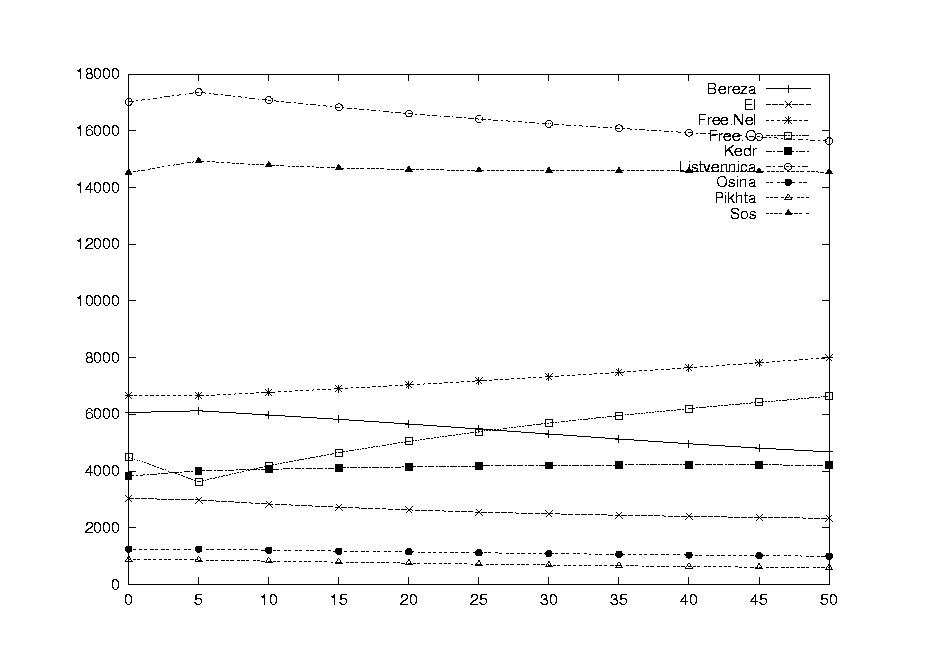
\includegraphics[width=17.12cm,height=11.649cm]{ReportIGForest2001-img002.png}
 

Рис. 4.4. График естественной и антропогенной временной динамики лесных ресурсов (1973-2023 гг.)

(Free Nel. – нелесная площадь, Free O. – непокрытая лесом площадь)

  [Warning: Image ignored] % Unhandled or unsupported graphics:
%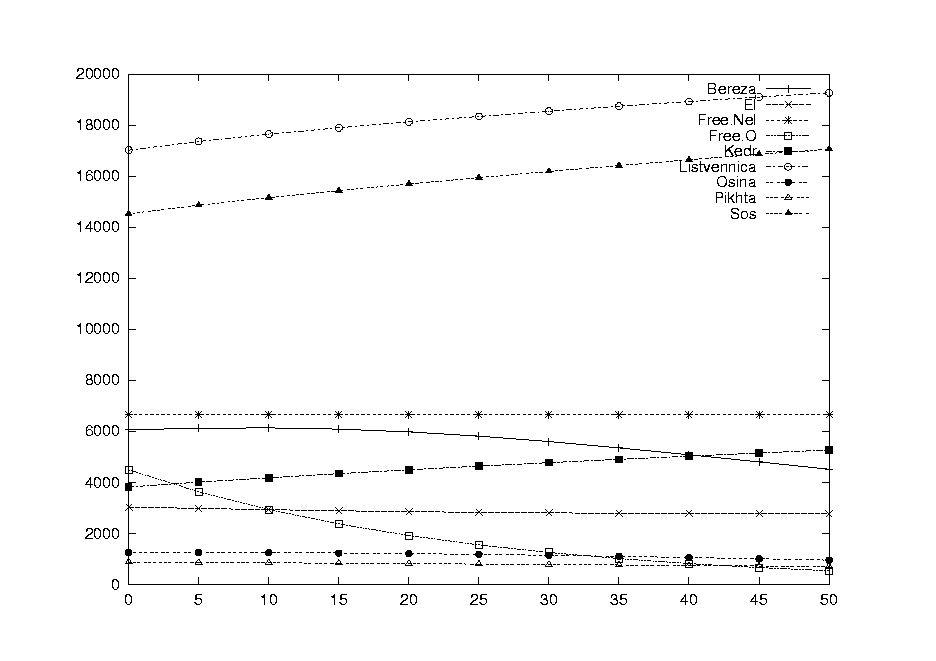
\includegraphics[width=17.12cm,height=11.335cm]{ReportIGForest2001-img003.png}
 

Рис. 4.5. График естественной временной динамики лесных ресурсов (1973-2023 гг.)

Согласно рис. 4.4. наиболее динамично изменяются площади лесов с преобладанием сосны, лиственницы и березы: площади
сосновых и лиственничных лесонасаждений уменьшаются в результате лесозаготовок, а березы – за счет преимущественного
восстановления этой порода на вырубках и гарях. На рис. 4.6. представлены расчетные и наблюдаемы значения этого
показателя. Хорошо видно, что расчетные и наблюдаемые характеристики совпадают, что говорит об адекватной работе модели
и возможности ее использования ее для прогнозных и оптимизационных расчетов. Небольшие неточности и отклонения вызваны
отсутствием данных о вырубках по породам по целому ряду лет и в связи с предположением, что рубки продолжались с
постоянным увеличением объемов заготовок древесины пропорционально площадям лесных массивов.

  [Warning: Image ignored] % Unhandled or unsupported graphics:
%\includegraphics[width=7.885cm,height=7.355cm]{ReportIGForest2001-img004.wmf}
 

\begin{center}
 [Warning: Image ignored] % Unhandled or unsupported graphics:
%\includegraphics[width=8.417cm,height=7.098cm]{ReportIGForest2001-img005.bmp}

\end{center}
Рис. 4.6. Сравнение расчетных и наблюдаемых характеристик динамики площадей лесов 

Иркутской области

В качестве одного из вариантов рассматривалась естественная динамика в отсутствии антропогенных воздействий (рис. 4.5).
Особенностью поведения лесной системы в данном случае является рост площадей лесов светлохвойных пород и кедра  и
снижение площади березовых лесов. Резко уменьшаются площади не покрытых лесом земель. Это отражает естественную с
экологической точки зрению и характерную для Иркутской области динамику лесонасаждений. 

Результаты работы докладывались на научной конференции [21].

На пути одновременного использования баз данных ГИС и баз данных моделей возникает ряд проблем, часть из которых связана
с совершенствованием расчетных схем, другие относятся на счет трудностей получения ведомственной информации нужного
качества и объема. Здесь необходимо решать дополнительные научные и организационные вопросы информационного обеспечения
управления лесными ресурсами.

5. БАЗА ДАННЫХ ПОКВАРТАЛЬНЫХ ИТОГОВ В СРЕДЕ ГИС ДЛЯ ЛЕСОСЫРЬЕВЫХ БАЗ И ЛЕСХОЗОВ ИРКУТСКОЙ ОБЛАСТИ

\ \ Средним уровнем геоинформационного обеспечения лесопользования являются данные квартальных итогов и соответствующие
им планы лесонасаждений.  Элементарной ячейкой управления здесь становится квартал, который считается однородным по
природным характеристикам участком лесной территории.  Основными переменными становятся площади и запасы лесонасаждений
с учетом их распределения по группам возраста. Квартальная сеть задает естественную систему координат, с помощью
которой все природные явления и лесохозяйственные мероприятия привязываются к местности, что позволяет организовывать
мониторинг и управление лесопользованием. Система кварталов определяет пространственную дифференциацию лесных ресурсов,
что лежит в основе планирования размещения  лесосек и картографирования состояния лесов по агрегированным показателям
как на текущий момент, так и с помощью моделей – на перспективу.  

5.1. Назначение базы данных поквартальных итогов

Информация такого рода формируется по результатам лесоустроительной инвентаризации лесов и содержится в ведомостях
поквартальных итогов разного содержания. Уровень пространственного разрешения  этих данных соответствует размеру
кварталов, что соответствует по разным категориям лесоустройства прямоугольникам 2x4 кв. км или 1х2 кв. км. Количество
кварталов в лесхозах исчисляется сотнями, что дает возможность анализировать лесную территорию как
пространственно-распределенную систему, решать задачи различной сложности. 

\ \ К числу проблем, которые могут обсуждаться на этом уровне генерализации данных можно отнести следующие. 

\begin{enumerate}
\item Привязка объектов собственности к координатам и линиям квартальной сети. 
\item Координация природных явлений и хозяйственных мероприятий по квартальной сети. 
\item Организация внутрирегионального дистанционного мониторинга с привязкой к квартальной сети.
\item Планирование процесса транспортного освоения территории. 
\item Проектирование размещения предприятий главного, дополнительного и побочного пользования. 
\item Выделение лесосырьевых баз лесозаготовительных предприятий. 
\item Получение справок о состоянии лесных ресурсов в границах кварталов.
\item Оценка лесных ресурсов по разным критериям использования и определение ущерба от пожаров, рубок и т.д. . 
\item Расчет функций полезности лесных угодий в аспекте их водорегулирующей, средоформирующей роли, а также поглощения
углекислого газа (оценка для углеродного квотирования).  
\item Картографирование распределения различных показателей состояния  лесных ресурсов по лесхозам и районам.  
\item Разработка алгоритмов дешифрирования аэрокосмической информации высокого и низкого разрешения для оперативного и
фонового мониторинга лесов области в целом и по отдельным районам. 
\item Осуществление оперативного и фонового мониторинга лесов области с использованием многозональной и радарной
информации. 
\item Корректировка данных поквартальных итогов на основе  космической информации.
\item Создание карт современного состояния и использования лесных ресурсов территории. 
\item Информационное обеспечения моделей для проведения прогнозных расчетов. 
\item Актуализация лесоустроительной информации по кварталам. 
\item Организация и проведение учета лесного фонда на уровне дробности квартальной сети. 
\item Контроль за использованием и местными потоками древесного сырья. 
\item Проведение  экологической экспертизы лесопользования с учетом местных географических условий и критериев
неистощительного лесопользования.  
\item Создание прогнозных карт освоения и использования лесных ресурсов территории. 
\item Обучение специалистов вариантному анализу стратегий пространственного освоения лесных ресурсов. 
\end{enumerate}
Создание ГИС поквартальных итогов Иркутской области обеспечивает наглядное отображение пространственной и временной
изменчивости состояний лесных ресурсов. Оперативное обновление такой информации на местах и представлением ее в
информационные центры области совместно с космическим мониторингом позволит перевести учет состояния лесных ресурсов на
более дробный уровень, что повысит качество контроля за их использованием и ответственность пользователей.  

5.2. ГИС поквартальных итогов

ГИС данных поквартальных итогов создана по образцу разработанной в Северо-западном лесоустроительном предприятии системы
WinEko. Это головное предприятие Леспроекта по созданию систем управления лесопользованием, поэтому предлагаемую ими
разработку следует считать модельной для создания региональных геоинформационных систем. 

ГИС предназначена для информационного обеспечения специалистов лесного хозяйства разнообразными справками о лесном фонде
севера Иркутской области из базы лесоустроительной информации на поквартальном уровне. Эта система обладает
возможностью дальнейшего совершенствования, расширения возможностей. 

Созданная геоинформационная система поквартальных итогов обеспечивает совмещение картографической базы данных с
лесоустроительной, на основе которой решаются задачи тематического картографирования с выбором окраски и формирования
необходимых  документов. 

Минимальным графическим объектом, по которому возможно получение содержательной информации, является квартал. Структура
поквартальной информации, используемая в системе, содержит основные агрегированные характеристики квартала.

Стандартная для ГИС-программ система выборок с двух направлений обеспечивает полноценный анализ лесного фонда.
Возможность выделения произвольного объекта в графике и выявление всех его лесоинвентаризационных характеристик, как и
обратная задача - создание объекта посредством выделения его по лесоинвентаризационным характеристикам и отображение
его в графике - позволяет пользователю получать полезную информацию.

Другой возможностью системы является окраска планов по произвольным характеристикам квартала или диаграммное
представление данных по выбираемому показателю в разрезе лесничеств.

ГИС поквартальных итогов предназначается для получения сведений о лесном фонде квартала, а также о любой совокупности
кварталов в лесничестве и лесхозе севера Иркутской области. Система допускает внесения текущих изменений в данные о
лесном фонде и замещение полностью обновленной базой. 

Для работы геоинформационной системы в эксплуатационном режиме рекомендуется компьютер не ниже возможностей Pentium II и
32 МБ оперативной памяти. Система работает с ОС Windows 95, 98, Millennium или с Windows NT (Workstation), 2000.

Структура баз данных представлена в табл. 5.1. 

Таблица 5.1. 

\subsection{Структура базы данных поквартальных итогов }
\begin{flushleft}
\tablefirsthead{}
\tablehead{}
\tabletail{}
\tablelasttail{}
\begin{supertabular}{|m{2.46cm}|m{8.761001cm}|m{2.023cm}|m{0.753cm}|m{2.049cm}|}
\hline
\centering{\selectlanguage{russian} Поле в Базе Данных} &
\centering{\selectlanguage{russian} Наименование} &
\centering{\selectlanguage{russian} Единица измерения} &
\centering{\selectlanguage{russian} Тип} &
{\centering\selectlanguage{russian} Кол-во\par}

\centering\arraybslash{\selectlanguage{russian} знаков}\\\hline
\centering{\selectlanguage{english} Region} &
{\selectlanguage{russian} Название области} &
 &
\centering{\selectlanguage{russian} С} &
\centering\arraybslash{\selectlanguage{english} 32}\\\hline
\centering{\selectlanguage{english} Cod\_Region} &
{\selectlanguage{russian} Код области} &
 &
\centering{\selectlanguage{russian} Ц} &
\centering\arraybslash{\selectlanguage{russian} 10}\\\hline
\centering{\selectlanguage{english} Raion} &
{\selectlanguage{russian} Название района} &
 &
\centering{\selectlanguage{russian} С} &
\centering\arraybslash{\selectlanguage{english} 32}\\\hline
\centering{\selectlanguage{english} Code\_Raion} &
{\selectlanguage{russian} Код района} &
 &
\centering{\selectlanguage{russian} Ц} &
\centering\arraybslash{\selectlanguage{russian} 5}\\\hline
\centering{\selectlanguage{english} Leshoz} &
{\selectlanguage{russian} Название лесхоза} &
 &
\centering{\selectlanguage{russian} С} &
\centering\arraybslash{\selectlanguage{english} 32}\\\hline
\centering{\selectlanguage{english} Cod\_Leshoz} &
{\selectlanguage{russian} Код лесхоза} &
 &
\centering{\selectlanguage{russian} Ц} &
\centering\arraybslash{\selectlanguage{russian} 8}\\\hline
\centering{\selectlanguage{english} Lesnich} &
{\selectlanguage{russian} Название лесничества} &
 &
\centering{\selectlanguage{russian} С} &
\centering\arraybslash{\selectlanguage{english} 32}\\\hline
\centering{\selectlanguage{english} Code\_Lesn} &
{\selectlanguage{russian} Код лесничества} &
 &
\centering{\selectlanguage{russian} Ц} &
\centering\arraybslash{\selectlanguage{russian} 10}\\\hline
\centering{\selectlanguage{english} Kvartal} &
{\selectlanguage{russian} Номер квартала} &
 &
\subsection{Ц}
 &
\centering\arraybslash{\selectlanguage{russian} 4}\\\hline
\centering{\selectlanguage{russian} Zaschit{}-t} &
{\selectlanguage{russian} Категория защитности} &
 &
\centering{\selectlanguage{english} C} &
\centering\arraybslash{\selectlanguage{russian} 32}\\\hline
\centering{\selectlanguage{english} ID} &
{\selectlanguage{russian} ГИС-идентификатор} &
 &
\centering{\selectlanguage{russian} Ц} &
\centering\arraybslash{\selectlanguage{russian} 16}\\\hline
\centering{\selectlanguage{english} Landscape} &
{\selectlanguage{russian} Тип ландшафта} &
 &
\centering{\selectlanguage{russian} С} &
\centering\arraybslash{\selectlanguage{english} 32}\\\hline
\centering{\selectlanguage{english} Prb\_S\_kind} &
{\selectlanguage{russian} Преобладающая по площади порода} &
 &
\centering{\selectlanguage{russian} С} &
\centering\arraybslash{\selectlanguage{english} 32}\\\hline
\centering{\selectlanguage{english} Prb\_W\_kind} &
{\selectlanguage{russian} Преобладающая по запасу порода} &
 &
\centering{\selectlanguage{russian} С} &
\centering\arraybslash{\selectlanguage{english} 32}\\\hline
\centering{\selectlanguage{english} Prb\_S\_GrVz} &
{\selectlanguage{russian} Преобладающая по площади группа возраста} &
 &
\centering{\selectlanguage{russian} С} &
\centering\arraybslash{\selectlanguage{russian} 32}\\\hline
\centering{\selectlanguage{english} Prb\_S\_Type} &
{\selectlanguage{russian} Преобладающий по площади тип леса} &
 &
\centering{\selectlanguage{russian} С} &
\centering\arraybslash{\selectlanguage{english} 32}\\\hline
\centering{\selectlanguage{english} S\_Lzem} &
{\selectlanguage{russian} Площадь лесных земель} &
{\selectlanguage{russian} Га} &
\centering{\selectlanguage{russian} Ц} &
\centering\arraybslash{\selectlanguage{english} 5}\\\hline
\centering{\selectlanguage{english} S\_L} &
{\selectlanguage{russian} Площадь покрытых лесом} &
{\selectlanguage{russian} Га} &
\centering{\selectlanguage{russian} Ц} &
\centering\arraybslash{\selectlanguage{english} 5}\\\hline
\centering{\selectlanguage{english} S\_SLk} &
{\selectlanguage{russian} Площадь сомкнувшихся лесных культур} &
{\selectlanguage{russian} Га} &
\centering{\selectlanguage{russian} Ц} &
\centering\arraybslash{\selectlanguage{english} 5}\\\hline
\centering{\selectlanguage{english} S\_NLk} &
{\selectlanguage{russian} Площадь несомкнувшихся лесных культур} &
{\selectlanguage{russian} Га} &
\centering{\selectlanguage{russian} Ц} &
\centering\arraybslash{\selectlanguage{english} 5}\\\hline
\centering{\selectlanguage{english} S\_LP} &
{\selectlanguage{russian} Площадь лесных питомников} &
{\selectlanguage{russian} Га} &
\centering{\selectlanguage{russian} Ц} &
\centering\arraybslash{\selectlanguage{english} 5}\\\hline
\centering{\selectlanguage{english} S\_redin} &
{\selectlanguage{russian} Площадь редин} &
{\selectlanguage{russian} Га} &
\centering{\selectlanguage{russian} Ц} &
\centering\arraybslash{\selectlanguage{english} 5}\\\hline
\centering{\selectlanguage{russian} S\_fire} &
{\selectlanguage{russian} Площадь гарей, погибших насаждений} &
{\selectlanguage{russian} Га} &
\centering{\selectlanguage{russian} Ц} &
\centering\arraybslash{\selectlanguage{english} 5}\\\hline
\centering{\selectlanguage{english} S\_cut} &
{\selectlanguage{russian} Площадь вырубок} &
{\selectlanguage{russian} Га} &
\centering{\selectlanguage{russian} Ц} &
\centering\arraybslash{\selectlanguage{english} 5}\\\hline
\centering{\selectlanguage{english} S\_glade} &
{\selectlanguage{russian} Площадь прогалин, пустырей} &
{\selectlanguage{russian} Га} &
\centering{\selectlanguage{russian} Ц} &
\centering\arraybslash{\selectlanguage{english} 5}\\\hline
\centering{\selectlanguage{english} S\_N} &
{\selectlanguage{russian} Площадь непокрытых лесом земель} &
{\selectlanguage{russian} Га} &
\centering{\selectlanguage{russian} Ц} &
\centering\arraybslash{\selectlanguage{english} 5}\\\hline
\centering{\selectlanguage{russian} S\_forest} &
{\selectlanguage{russian} Площадь лесных земель} &
{\selectlanguage{russian} Га} &
\centering{\selectlanguage{russian} Ц} &
\centering\arraybslash{\selectlanguage{english} 5}\\\hline
\centering{\selectlanguage{english} S\_arable} &
{\selectlanguage{russian} Площадь пашен} &
{\selectlanguage{russian} Га} &
\centering{\selectlanguage{russian} Ц} &
\centering\arraybslash{\selectlanguage{english} 5}\\\hline
\centering{\selectlanguage{english} S\_hay} &
{\selectlanguage{russian} Площадь сенокосов} &
{\selectlanguage{russian} Га} &
\centering{\selectlanguage{russian} Ц} &
\centering\arraybslash{\selectlanguage{english} 5}\\\hline
\centering{\selectlanguage{english} S\_pasture} &
{\selectlanguage{russian} Площадь пастбищ} &
{\selectlanguage{russian} Га} &
\centering{\selectlanguage{russian} Ц} &
\centering\arraybslash{\selectlanguage{english} 5}\\\hline
\centering{\selectlanguage{english} S\_water} &
{\selectlanguage{russian} Площадь вод} &
{\selectlanguage{russian} Га} &
\centering{\selectlanguage{russian} Ц} &
\centering\arraybslash{\selectlanguage{english} 5}\\\hline
\centering{\selectlanguage{english} S\_road} &
{\selectlanguage{russian} Площадь дорог и просек} &
{\selectlanguage{russian} Га} &
\centering{\selectlanguage{russian} Ц} &
\centering\arraybslash{\selectlanguage{english} 5}\\\hline
\centering{\selectlanguage{english} S\_house} &
{\selectlanguage{russian} Площадь усадеб и пр. земель} &
{\selectlanguage{russian} Га} &
\centering{\selectlanguage{russian} Ц} &
\centering\arraybslash{\selectlanguage{english} 5}\\\hline
\centering{\selectlanguage{english} S\_bog} &
{\selectlanguage{russian} Площадь болот} &
{\selectlanguage{russian} Га} &
\centering{\selectlanguage{russian} Ц} &
\centering\arraybslash{\selectlanguage{english} 5}\\\hline
\centering{\selectlanguage{english} S\_other} &
{\selectlanguage{russian} Прочие земли} &
{\selectlanguage{russian} Га} &
\centering{\selectlanguage{russian} Ц} &
\centering\arraybslash{\selectlanguage{english} 5}\\\hline
\centering{\selectlanguage{russian} S\_noforest} &
{\selectlanguage{russian} Площадь лесных земель} &
{\selectlanguage{russian} Га} &
\centering{\selectlanguage{russian} Ц} &
\centering\arraybslash{\selectlanguage{english} 5}\\\hline
\centering{\selectlanguage{english} W\_All} &
{\selectlanguage{russian} Общий запас насаждения} &
{\selectlanguage{russian} Дес. м3} &
\centering{\selectlanguage{russian} Ц} &
\centering\arraybslash{\selectlanguage{russian} 7}\\\hline
\centering{\selectlanguage{russian} W\_redin} &
{\selectlanguage{russian} Запас редин} &
{\selectlanguage{russian} Дес. м3} &
\centering{\selectlanguage{russian} Ц} &
\centering\arraybslash{\selectlanguage{russian} 5}\\\hline
\centering{\selectlanguage{russian} W\_ones} &
{\selectlanguage{russian} Запас единичн. деревьев} &
{\selectlanguage{russian} Дес. м3} &
\centering{\selectlanguage{russian} Ц} &
\centering\arraybslash{\selectlanguage{russian} 5}\\\hline
\centering{\selectlanguage{russian} W\_growth} &
{\selectlanguage{russian} Запас сырорастущего} &
{\selectlanguage{russian} Дес. м3} &
\centering{\selectlanguage{russian} Ц} &
\centering\arraybslash{\selectlanguage{english} 7}\\\hline
\centering{\selectlanguage{english} W\_new\_dry} &
{\selectlanguage{russian} Запас свежего сухостоя} &
{\selectlanguage{russian} Дес. м3} &
\centering{\selectlanguage{russian} Ц} &
\centering\arraybslash{\selectlanguage{russian} 5}\\\hline
\centering{\selectlanguage{russian} W\_dry} &
{\selectlanguage{russian} Запас сухостоя} &
{\selectlanguage{russian} Дес. м3} &
\centering{\selectlanguage{russian} Ц} &
\centering\arraybslash{\selectlanguage{russian} 5}\\\hline
\centering{\selectlanguage{english} Stuff} &
{\selectlanguage{russian} Захламленность} &
{\selectlanguage{russian} Дес. м3} &
\centering{\selectlanguage{russian} Ц} &
\centering\arraybslash{\selectlanguage{english} 5}\\\hline
\centering{\selectlanguage{english} Stuff\_Likv} &
{\selectlanguage{russian} Захламленность ликвида} &
{\selectlanguage{russian} Дес. м3} &
\centering{\selectlanguage{russian} Ц} &
\centering\arraybslash{\selectlanguage{english} 5}\\\hline
\centering{\selectlanguage{english} S\_Pris} &
{\selectlanguage{russian} Площадь приспевающих} &
{\selectlanguage{russian} Га} &
\centering{\selectlanguage{russian} Ц} &
\centering\arraybslash{\selectlanguage{english} 5}\\\hline
\centering{\selectlanguage{english} W\_Pris} &
{\selectlanguage{russian} Запас приспевающих} &
{\selectlanguage{russian} Дес. м3} &
\centering{\selectlanguage{russian} Ц} &
\centering\arraybslash{\selectlanguage{english} 5}\\\hline
\centering{\selectlanguage{english} S\_SpPer} &
{\selectlanguage{russian} Площадь спелых и перестойных} &
{\selectlanguage{russian} Га} &
\centering{\selectlanguage{russian} Ц} &
\centering\arraybslash{\selectlanguage{english} 5}\\\hline
\centering{\selectlanguage{english} W\_SpPer} &
{\selectlanguage{russian} Запас спелых и перестойных} &
{\selectlanguage{russian} Дес. м3} &
\centering{\selectlanguage{russian} Ц} &
\centering\arraybslash{\selectlanguage{english} 5}\\\hline
\centering{\selectlanguage{english} W\_SpPer\_S} &
{\selectlanguage{russian} Запас спелых и перестойных по сосне} &
{\selectlanguage{russian} Дес. м3} &
\centering{\selectlanguage{russian} Ц} &
\centering\arraybslash{\selectlanguage{english} 5}\\\hline
\centering{\selectlanguage{english} W\_SpPer\_E} &
{\selectlanguage{russian} Запас спелых и перестойных по еле} &
{\selectlanguage{russian} Дес. м3} &
\centering{\selectlanguage{russian} Ц} &
\centering\arraybslash{\selectlanguage{russian} 5}\\\hline
\centering{\selectlanguage{english} W\_SpPer\_P} &
{\selectlanguage{russian} Запас спелых и перестойных по пихте} &
{\selectlanguage{russian} Дес. м3} &
\centering{\selectlanguage{russian} Ц} &
\centering\arraybslash{\selectlanguage{english} 5}\\\hline
\centering{\selectlanguage{english} W\_SpPer\_L} &
{\selectlanguage{russian} Запас спелых и перестойных по лиственнице} &
{\selectlanguage{russian} Дес. м3} &
\centering{\selectlanguage{russian} Ц} &
\centering\arraybslash{\selectlanguage{english} 5}\\\hline
\centering{\selectlanguage{english} W\_SpPer\_K} &
{\selectlanguage{russian} Запас спелых и перестойных по кедра} &
{\selectlanguage{russian} Дес. м3} &
\centering{\selectlanguage{russian} Ц} &
\centering\arraybslash{\selectlanguage{english} 5}\\\hline
\centering{\selectlanguage{english} W\_SpPer\_B} &
{\selectlanguage{russian} Запас спелых и перестойных по березе} &
{\selectlanguage{russian} Дес. м3} &
\centering{\selectlanguage{russian} Ц} &
\centering\arraybslash{\selectlanguage{english} 5}\\\hline
\centering{\selectlanguage{english} W\_SpPer\_Os} &
{\selectlanguage{russian} Запас спелых и перестойных по осине} &
{\selectlanguage{russian} Дес. м3} &
\centering{\selectlanguage{russian} Ц} &
\centering\arraybslash{\selectlanguage{russian} 5}\\\hline
\end{supertabular}
\end{flushleft}
Список включенных в базу данных переменных достаточно обширен, но не исчерпывает всех необходимых для управления
характеристик. Например, отсутствуют как самостоятельные значения запасы леса на гектар, картографическое представление
которых дает информацию о плотности лесных ресурсов. Для прогнозных расчетов необходимы сведения о возрасте рубки, на
основе которых происходит выделение лесонасаждений разных групп возраста. С другой стороны, часть показателей, особенно
касающихся структуры не покрытых лесом и нелесных площадей, явно являются избыточными. Формирующаяся база данных
поквартальных итогов для Иркутской области должна содержать, прежде всего, ту информацию, которая необходима для
дистанционного космического мониторинга лесов, текущего учета состояния лесного фонда и прогнозирования динамики.  

5.3. Базы данных поквартальных итогов и их картографическое отображение

Таблицы поквартальных итогов в проектах организации лесного хозяйства формируются на основе повыделенных
лесотаксационных описаний. Потенциально они могут в средних и агрегированных показателях содержать весь список
характеристик выделов, что станет практически возможным при создании специализированны баз данных и ГИС, содержащих
повыделенную информацию. В настоящее время в Иркутской области существуют подобные ГИС Слюдянского и Голоустинского
лесхозов (Прибайкальское лесоустроительное предприятие), ГИС лесов о. Ольхон (Иркутский комитет по охране окружающей
среды), ГИС лесов Слюдянского района, включая часть Прибайкалького национального парка (Институт географии СО РАН).  В
Прибайкальском лесорустроительном предприятии за последние 20 лет накопилась повыделенная  большая информация о многих
лесхозах, устроенных за этот период предприятием. На их основе при соответствующей финансовой поддержке могут быть
созданы эффективные ГИС лесхозов. К сожалению при подготовке ГИС-проектов этого типа сейчас используются разные
программные продукты (ARC{}-INFO, ArcView, WinGIS) с неодинаковыми возможностями обработки данных на различной основе
картосоставления.  

При создании ГИС поквартальных итогов лесхозов севера Иркутской области была сделана попытка реализовать опытный вариант
ГИС лесной таксации в программной среде КАМАТ, привязав лесотаксационные выделы к электронной топографической карте
российского образца.  

Процедура создания ГИС поквартальных итогов состоит из следующих этапов: 

\begin{enumerate}
\item привязка реперных точек кварталов к геодезическим координатам; 
\item нанесение на бумажную топографическую основу квартальной сети в соответствии с планами лесонасаждений и
лесоустроительными планшетами; 
\item цифрование картографического материала с векторизацией изображений квартальной сети;
\item картографическая привязка оцифрованных изображений;  
\item создание базы данных поквартальных итогов; 
\item присоединение базы данных к полигонам тематического слоя “Квартальная сеть”; 
\item визуализация базы данных по тематическим слоям в соответствии с запросами пользователя.  
\end{enumerate}
В материалах поквартальных итогов содержится информация о распределении площади квартала по категориям земель, площади и
запасов лесов по породам и группам возраста, о средних таксационных характеристиках.  

Картографически эти показатели отображаются стандартным образом, окрашивая в соответствии с градацией признака ареал
каждого квартала в определенный цвет. На рис. 5.1 для примера показана карта запаса спелых и перестойных лесов
Воробьевского и Ершовского лесничеств Эдучанского лесхоза Усть-Илимского района. 

5.4. Информационное обеспечение задач прогнозирования

\ \ Данные поквартальных итогов описанной выше структуры содержат достаточно информации для информационного обеспечения
математических моделей внутрирегионального уровня, описанных в разделе 1.3. Они позволят провести более детальную
структуризацию расчетной схемы с учетом породного состава лесонасаждений, а значит дадут возможность учесть
закономерности смены пород, столь характерные для таежных лесов Иркутской области, где часто возобновление коренных
лесов идет через древостои мелколиственных пород. 

\ \  ГИС квартальной сети позволяет вместо регулярной сетки интегрирования использовать в качестве основы дискретизации
пространства квартальную нерегулярную сеть. Практически это не слишком осложняет вычисления, но позволяет результаты
расчетов использовать в том же режиме, что и исходные данные, визуализировать их как обычные базы данных поквартальных
итогов. Все это привносит в расчеты практический смысл, позволяет использовать результаты космического мониторинга для
коррекции информации и т.д. 

\ \ Таким образом, предполагается что расчеты будут осуществляться на имеющейся базе данных, и получается обновленная
(актуализированная) база данных, которая визуализируется в общем режиме. Последовательное подключение данных разных
этапов прогноза позволит получить картографическую анимацию, отображающую изменение во времени и в пространстве
различных характеристик лесов. 

6. РАСЧЕТ УЩЕРБА, ПРИЧИНЕННОГО УНИЧТОЖЕНИЕМ ИЛИ ПОВРЕЖДЕНИЕМ ЛЕСА В РЕЗУЛЬТАТЕ ПОДЖОГО ИЛИ НЕБРЕЖНОГО ОБРАЩЕНИЯ С ОГНЕМ

ЗАКЛЮЧЕНИЕ

Работы всех этапов выполнены в полном объеме и в сроки, предусмотренные календарным планом.

В плане работ по созданию новых информационных технологий планирования и  управления  лесными ресурсами Иркутской
области выделен  круг  проблем,  которые  необходимо решать в первую очередь. К числу таких проблем относится
организация эффективного контроля за использованием лесных ресурсов. С этой целью разрабона система информационного
ГИС-обеспечения лесопользования и охраны лесов и комплекс математических моделей, в задачу которого входит оценка
эффективности проведения лесохозяйственных мероприятий через прогноз последствий их реализации в конкретных
экологических условиях и географических положениях. Разработана система математических моделей, создана компьютерная
программа Forest resources{}-3, предназначенная для расчета временной динамики лесных ресурсов территории с
детальностью стандартных форм учета лесного фонда. Проведена проверка адекватности модели на конкретных данных
изменения состояния лесного фонда Иркутской области, начиная с 73-го года, по категориям земель, площадей и запасов
лесов по породам и группам возраста с учетом различного вида хозяйственной деятельности и катастрофических смен (рубок,
пожаров). И в ходе запланированных исследований решена задача их информационного обеспечения применительно к условиям
области.  Это дает возможность полнее использовать лесоустроительную информацию для прогнозных целей и оперативно
принимать решения по использованию лесосырьевых баз в диалоге с персональным компьютером.

В комплексе программ предлагаются модели двух основных уровней: модели внутрирегионального уровня и модели локального
уровня.

Первые  касаются  прогнозирования  динамики  лесных  ресурсов участков лесосырьевой базы в терминах изменения
распределения площадей по породам, классам возраста, запасу и т.д. с учетом разнообразных лесохозяйственных
мероприятий, связанных с изменение состояния лесных площадей (рубки главного пользования, формирование лесных культур и
т.д.).

Второй класс моделей направлен на оценку эффективности выборочных рубок и рубок ухода. Смысл расчетов заключается в
определении изменения распределения деревьев  в  древостое по размерам. 

Модели основаны на фундаментальных закономерностях смены состояний таежных экосистем и предназначены для оценки
последствий хозяйственной деятельности в различных районах Иркутской области.

Для информационного обеспечения расчетных схем и решения других важных практических задач лесопользования созданаГИС
состояния  лесного фонда (ГИС СЛФ) на различных уровнях агрегирования лесоустроительной информации. 

Система моделей естественно вписывается в процедуры ГИС, позволяя наглядно представлять последствия хозяйственных
мероприятий. Комплекс программ рассматривается как составная часть программного обеспечения геоинформационных систем
для органов государственной власти (ГИС ОГВ). Он позволит хранить лесоустроительную информацию, преобразовывать ее для
решения задач прогнозирования и проводить прогнозные расчеты для лесных массивов разного масштаба с учетом особенностей
лесорастительных условий, лесозаготовок, пожаров и других факторов воздействия на лес. Результаты расчетов будут
отображаются на экран компьютера в виде графиков и прогнозных карт. 

На основе имеющейся информации учета лесного фонда и поквартальных итогов разработана серия справочно-аналитических
карт, отображающих разные характеристики состояния лесных ресурсов Иркутской области в разрезе районов, лесхозов и
кварталов. Проведен системный анализ картографического материала с целью определения перспективных направлений
инвестиций в лесной комплекс области. Показаны возможности вариантных расчетов для оценки воздействия планируемых
хозяйственных мероприятий на природную среду. 

ЛИТЕРАТУРА

\begin{enumerate}
\item  Россия. Лесная политика в переходный период. Региональные исследования всемирного банка. - 1997. - 336 С.
\item  Моделирование процессов в природно-экономических системах. -Новосибирск: Наука,1982.- 176 С.
\item  Модели управления природными ресурсами. - М.: Наука, 1981.- 264 С.
\item  Эколого-экономические системы: модели, информация, эксперимент. -Новосибирск: Наука,1987.-216 С.
\item  Черкашин А.К. Динамическая модель сукцессии пихтовой тайги//Модели природных систем.- Новосибирск: Наука,
1978.-С. 94-99.
\item  Батурин В.А., Данилина Е.В.,Сидоренко Г.В., Черкашин А.К. Задача нормирования нагрузки на лесной комплекс// Новые
методы улучшения управляемых процессов.-Новосибирск: Наука, 1987.- С. 160-163.
\item  Говорин В.П., Данилина Е.В., Москаленко А.И., Чемезова Т.В.,Черкашин А.К. Модели и методы для оценки и повышения
экологической и экономической эффективности планирования использования лесных ресурсов Иркутской области //
Природно-ресурсный потенциал Восточной Сибири и проблемы формирования аграрных и промышленных комплексов.- Иркутск,
1986.- С. 123-124.
\item  Москаленко А.И., Черкашин А.К. Модель пространственной и возрастной структуры леса //Модели управления природными
ресурсами.-М.: Наука, 1981.- С. 231-243.
\item  Москаленко А.И., Черкашин А.К.,Бутин А.А., Душин К.Б., Овсянникова Н.А. Расчет оптимальной структуры
древостоя//Эколого-экономическая стратегия развития региона. Математическое моделирование и системный анализ на примере
Байкальского региона.-Новоси-бирск:. Наука: 1990.-С.129-135.
\item  Рагозин А.В., Черкашин А.К. Прогнозирование пространственно-временной динамики леса на основе математической
модели  с распределенными  параметрами //  Планирование  и прогнозирование природно-экономических систем.-Новосибирск:
Наука, 1984.-С.58-68.
\item  Раздьяконова Т.С., Черкашин А.К., Шепотько И.О Планирование лесозаготовок с учетом пространственно-временной
динамики лесных ресурсов (на примере лесов зоны БАМа) // Планирование и прогнозирование природно-экономических
систем.-Новосибирск: Наука, 1984.-С.81-88.
\item  Черкашин А.К. Прогноз пространственной и временной динамики лесов таежного ландшафта// Динамика
эколого-экономических систем.-Новосибирск: Наука, 1981.- С.107-111.
\item  Черкашин А.К. Составление таблиц хода роста сложных лесонасаждений на основе математической модели//
Моделирование процессов в природно-экономических системах.-Новосибирск: Наука, 1982.- С.45-55.
\item  Черкашин А.К. Модель динамики лесонасаждений лесхоза и ее применение для решения прогнозных задач// Планирование
и прогнозирование природно-экономических систем.-Новосибирск: Наука, 1984.-С.69-81.
\item  Черкашин А.К. Система математических моделей леса// Планирование и прогнозирование природно-экономических систем.
-Новосибирск: Наука, 1984.-С.46-57
\item  Черкашин А.К. Методика определения параметров блока {\textquotedbl}Лесные
ресурсы{\textquotedbl}//Эколого-экономическая стратегия развития региона. Математическое моделирование и системный
анализ на примере Байкальского региона. - Новосибирск: Наука: 1990.-С.34-55.
\item  Владимиров И.Н. Модели динамики лесных экосистем ландшафтного уровня // Экология ландшафта и планирование
землепользования: Тезисы докладов Всероссийской конференции (Иркутск, 11-12 сентября 2000г.) - Новосибирск: Изд-во СО
РАН, 2000. - С. 49-51.
\item  Владимиров И.Н. ГИС состояния лесного фонда Иркутской области// VII научное совещание по прикладной географии:
Тезисы научной конференции (Иркутск, 22-23 мая 2001г.) - Иркутск: Изд-во Института географии СО РАН, 2001. - С.
191-193.
\item  Владимиров И.Н. ГИС в решении задач прогнозирования динамики лесных ресурсов// Дендрологические исследования в
Байкальской Сибири. - Иркутск: СИФИБР СО РАН, 2001. - С. 100-101.
\item  Владимиров И.Н., Черкашин Е.А. Геоинформационная система состояния и прогнозирования естественной и антропогенной
динамики лесных ресурсов Иркутской области// Математическое моделирование и информационные технологии: состояние и
перспективы: Тезисы докладов школы-семинара (Иркутск - Аршан, 12-17 октября 2001г.) - Иркутск: Институт динамики систем
и теории управления СО РАН, 2001. - С. 8-9.
\item  Владимиров И.Н., Черкашин А.К., Черкашин Е.А. Динамика лесных ресурсов административной территории: проверка
адекватности модели и прогноз// География Азиатской России на рубеже веков. Материалы XI научного совещания географов
Сибири и Дальнего Востока. – Иркутск: Изд-во Института географии СО РАН, 2001. - С. 200.
\item  Python Documentation (Release 2.0) /Guido van Rossum, Fred L. Drake, Jr., editor, - BeOpen PythonLabs. - 2000
\end{enumerate}
\section{ПРИЛОЖЕНИЕ 1}
РАСЧЕТ СРЕДНЕГО ВОЗРАСТА РАЗРУШЕНИЯ ПЕРЕСТОЙНЫХ 

ЛЕСОВ

В математической модели, предназначенной для расчета временной динамики лесных ресурсов территории различного породного
состава, отражена естественная смена пород. При этом подразумевается, что перестойные леса лиственных пород
преимущественно заменяются средневозрастными лесами хвойных пород в направлениях, отражающих экологическую ситуацию
территории, конкурентоспособность разных лесообразующих видов деревьев в конкретной географической среде в границах
Иркутской области.

При расчете интенсивности разрушения перестойных лесов со сменой пород необходимо рассчитать среднее время ($\tau $i6)
разрушения перестойных лесов каждой i{}-ой породы. При его определении будем исходить из гипотезы, что площади
перестойных лесов в первом приближении убывают по экспоненциальной зависимости, имеющей дифференциальное выражение: 

 $\frac{\normalsubformula{\text{dS}}_{\mathit{i6}}}{\normalsubformula{\text{dt}}}=-\lambda
_{\mathit{i6}}\mathit{Salignl}\begin{matrix}?\mathit{i6}\\?_{}\\?\end{matrix}$,  (1.1)

где $\lambda $i6 = 1/$\tau $i6. Время t = $\Delta $$\tau $i·n, где $\Delta $$\tau $i – шаг деления на классы возраста, n
– номер класса возраста. Решение (1.1) при этих условиях дает экспоненциальную зависимость (рис.1.1)

 $S_{6i}\left(n\right)=S_{0i}e^{-k_in}$,\ \   (1.2)

где S0i  {}- некоторая константа, соответствующая площади лесонасаждений в начальном классе возраста при условии, что
разрушение лесов шло на всем возрастном интервале по тем же самым принципам что и в перестойных насаждениях. Это
предположение не имеет особого значения и принято для удобства статистических расчетов. Коэффициент ki = $\Delta $$\tau
$i/$\Delta $$\tau $i6. Отсюда $\Delta $$\tau $i6 = $\Delta $$\tau $i/ki.

Коэффициенты ki и S0i рассчитываются методами линейной регрессии по схеме, полученной из уравнения (1.2) после
логарифмирования:

 $\text{ln}S_{6i}\left(n\right)=\text{ln}S_{0i}-k_in$.  (1.3)

Результаты расчетов коэффициентов представлены в табл. 1.1. Использовались данные лесоустройства (итоговые таблицы
распределения площадей лесов по породам и классам возраста) различных лесхозов Иркутской области.

  [Warning: Image ignored] % Unhandled or unsupported graphics:
%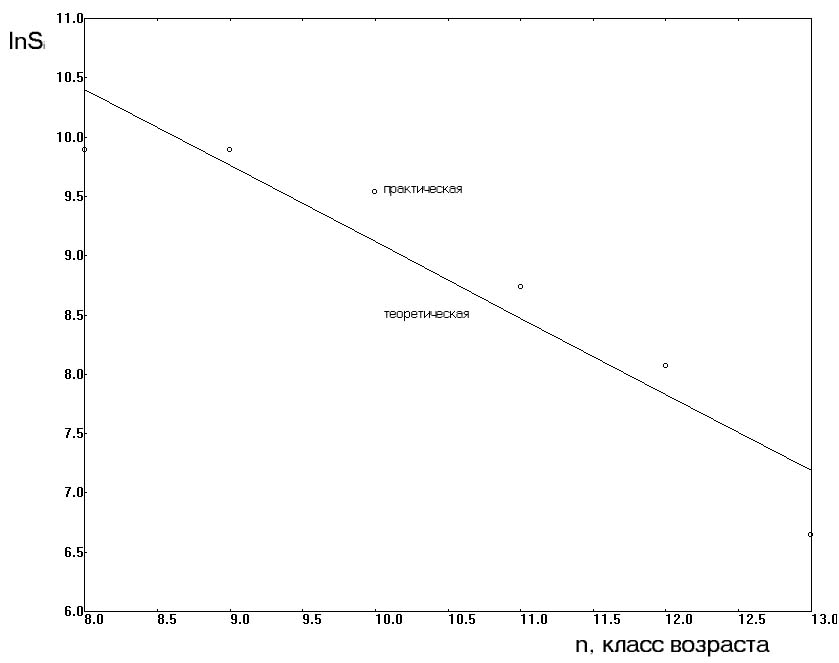
\includegraphics[width=16.958cm,height=13.4cm]{ReportIGForest2001-img006.jpg}
 

Рис. 1.1. Разрушение перестойных древостоев сосны в Шестаковском лесхозе Иркутской области

Расчеты среднего возраста разрушения перестойных лесов, приведенные в таблице 1.1, проводились на персональном
компьютере с помощью программ Microsoft Excel и RAKE (Regression mAKEr). 

Средний возраст разрушения перестойных лесов по породам в целом по Иркутской области находится как среднее
арифметическое найденных средних возрастов для лесхозов.

Получены следующие результаты по породам:  

\begin{itemize}
\item Сосна - 48,1лет;
\item Лиственница - 50,1 лет;
\item Кедр - 78,9 лет;
\item Ель - 24,9 лет;
\item Пихта - 17,3 лет;
\item Береза - 12,0 лет;
\item Осина - 15,4 лет.
\end{itemize}
Эти данные использовались для расчета интенсивности разрушения перестойных насаждений по формуле (4.13).

Таблица 1.1. 

Расчет среднего времени разрушения перестойных лесов в отдельных лесхозах Иркутской области

\begin{flushleft}
\tablefirsthead{}
\tablehead{}
\tabletail{}
\tablelasttail{}
\begin{supertabular}{|m{2.723cm}|m{2.5149999cm}|m{2.065cm}|m{3.0049999cm}|m{1.52cm}|m{1.673cm}|m{2.158cm}|}
\hline
\centering{\selectlanguage{russian} Лесхоз} &
\centering{\selectlanguage{russian} Порода} &
{\centering\selectlanguage{russian} Начальный класс возраста,\par}

\centering{\selectlanguage{russian} nнач} &
\centering{\selectlanguage{russian} Коэффициент корреляции, R} &
\centering{\selectlanguage{russian} lnS0i} &
\centering{\selectlanguage{english} k} &
\centering\arraybslash{\selectlanguage{russian} Время разрушения, $\tau $}\\\hline
{\selectlanguage{russian} Заярский} &
{\selectlanguage{russian} сосна} &
\centering{\selectlanguage{russian} 4} &
\centering{\selectlanguage{russian} 0,884112407} &
\centering{\selectlanguage{russian} 11,3617} &
\centering{\selectlanguage{russian} {}-0,32016} &
\centering\arraybslash{\selectlanguage{russian} 62,46818}\\\hline
 &
{\selectlanguage{russian} лиственница} &
\centering{\selectlanguage{russian} 4} &
\centering{\selectlanguage{russian} 0,719744348} &
\centering{\selectlanguage{russian} 10,253} &
\centering{\selectlanguage{russian} {}-0,23872} &
\centering\arraybslash{\selectlanguage{russian} 83,77946}\\\hline
 &
{\selectlanguage{russian} кедр} &
\centering{\selectlanguage{russian} 7} &
\centering{\selectlanguage{russian} 0,800356571} &
\centering{\selectlanguage{russian} 9,34511} &
\centering{\selectlanguage{russian} {}-0,29908} &
\centering\arraybslash{\selectlanguage{russian} 133,7435}\\\hline
 &
{\selectlanguage{russian} ель} &
\centering{\selectlanguage{russian} 8} &
\centering{\selectlanguage{russian} 0,945864656} &
\centering{\selectlanguage{russian} 17,3268} &
\centering{\selectlanguage{russian} {}-1,20867} &
\centering\arraybslash{\selectlanguage{russian} 16,54711}\\\hline
 &
{\selectlanguage{russian} пихта} &
\centering{\selectlanguage{russian} 6} &
\centering{\selectlanguage{russian} 0,923190968} &
\centering{\selectlanguage{russian} 11,974} &
\centering{\selectlanguage{russian} {}-0,74048} &
\centering\arraybslash{\selectlanguage{russian} 27,00958}\\\hline
 &
{\selectlanguage{russian} береза} &
\centering{\selectlanguage{russian} 7} &
\centering{\selectlanguage{russian} 0,974579401} &
\centering{\selectlanguage{russian} 19,7804} &
\centering{\selectlanguage{russian} {}-1,28959} &
\centering\arraybslash{\selectlanguage{russian} 7,754403}\\\hline
 &
{\selectlanguage{russian} осина} &
\centering{\selectlanguage{russian} 7} &
\centering{\selectlanguage{russian} 0,984818932} &
\centering{\selectlanguage{russian} 14,9356} &
\centering{\selectlanguage{russian} {}-0,80857} &
\centering\arraybslash{\selectlanguage{russian} 12,36756}\\\hline
 &
 &
 &
 &
 &
 &
\\\hline
{\selectlanguage{russian} Аларский} &
{\selectlanguage{russian} сосна} &
\centering{\selectlanguage{russian} 3} &
\centering{\selectlanguage{russian} 0,92758698} &
\centering{\selectlanguage{russian} 10,0673} &
\centering{\selectlanguage{russian} {}-0,53225} &
\centering\arraybslash{\selectlanguage{russian} 37,57612}\\\hline
 &
{\selectlanguage{russian} лиственница} &
\centering{\selectlanguage{russian} 6} &
\centering{\selectlanguage{russian} 0,935524343} &
\centering{\selectlanguage{russian} 16,2137} &
\centering{\selectlanguage{russian} {}-1,53532} &
\centering\arraybslash{\selectlanguage{russian} 13,0266}\\\hline
 &
{\selectlanguage{russian} кедр} &
 &
 &
 &
 &
\\\hline
 &
{\selectlanguage{russian} ель} &
 &
 &
 &
 &
\\\hline
 &
{\selectlanguage{russian} пихта} &
 &
 &
 &
 &
\\\hline
 &
{\selectlanguage{russian} береза} &
\centering{\selectlanguage{russian} 5} &
\centering{\selectlanguage{russian} 0,974935202} &
\centering{\selectlanguage{russian} 14,8216} &
\centering{\selectlanguage{russian} {}-1,29915} &
\centering\arraybslash{\selectlanguage{russian} 7,697341}\\\hline
 &
{\selectlanguage{russian} осина} &
\centering{\selectlanguage{russian} 4} &
\centering{\selectlanguage{russian} 0,998335292} &
\centering{\selectlanguage{russian} 6,79287} &
\centering{\selectlanguage{russian} {}-0,77022} &
\centering\arraybslash{\selectlanguage{russian} 12,98327}\\\hline
 &
 &
 &
 &
 &
 &
\\\hline
{\selectlanguage{russian} Баерский} &
{\selectlanguage{russian} сосна} &
\centering{\selectlanguage{russian} 3} &
\centering{\selectlanguage{russian} 0,682432266} &
\centering{\selectlanguage{russian} 10,8084} &
\centering{\selectlanguage{russian} {}-0,23563} &
\centering\arraybslash{\selectlanguage{russian} 84,87956}\\\hline
 &
{\selectlanguage{russian} лиственница} &
\centering{\selectlanguage{russian} 3} &
\centering{\selectlanguage{russian} 0,868088216} &
\centering{\selectlanguage{russian} 9,21778} &
\centering{\selectlanguage{russian} {}-0,21776} &
\centering\arraybslash{\selectlanguage{russian} 91,84592}\\\hline
 &
{\selectlanguage{russian} кедр} &
\centering{\selectlanguage{russian} 5} &
\centering{\selectlanguage{russian} 0,075011916} &
\centering{\selectlanguage{russian} 6,31856} &
\centering{\selectlanguage{russian} 0,11862} &
\centering\arraybslash{\selectlanguage{russian} 337,2198}\\\hline
 &
{\selectlanguage{russian} ель} &
\centering{\selectlanguage{russian} 7} &
\centering{\selectlanguage{russian} 0,961502504} &
\centering{\selectlanguage{russian} 23,1273} &
\centering{\selectlanguage{russian} {}-1,8315} &
\centering\arraybslash{\selectlanguage{russian} 10,92001}\\\hline
 &
{\selectlanguage{russian} пихта} &
\centering{\selectlanguage{russian} 6} &
\centering{\selectlanguage{russian} 0,950361545} &
\centering{\selectlanguage{russian} 20,4057} &
\centering{\selectlanguage{russian} {}-1,6412} &
\centering\arraybslash{\selectlanguage{russian} 12,18621}\\\hline
 &
{\selectlanguage{russian} береза} &
\centering{\selectlanguage{russian} 5} &
\centering{\selectlanguage{russian} 0,966084227} &
\centering{\selectlanguage{russian} 15,9474} &
\centering{\selectlanguage{russian} {}-0,9859} &
\centering\arraybslash{\selectlanguage{russian} 10,14306}\\\hline
 &
{\selectlanguage{russian} осина} &
\centering{\selectlanguage{russian} 5} &
\centering{\selectlanguage{russian} 0,898952293} &
\centering{\selectlanguage{russian} 12,2284} &
\centering{\selectlanguage{russian} {}-0,65837} &
\centering\arraybslash{\selectlanguage{russian} 15,18914}\\\hline
 &
 &
 &
 &
 &
 &
\\\hline
{\selectlanguage{russian} Бирюсинский} &
{\selectlanguage{russian} сосна} &
\centering{\selectlanguage{russian} 8} &
\centering{\selectlanguage{russian} 0,895560512} &
\centering{\selectlanguage{russian} 13,4462} &
\centering{\selectlanguage{russian} {}-0,31876} &
\centering\arraybslash{\selectlanguage{russian} 62,74313}\\\hline
 &
{\selectlanguage{russian} лиственница} &
\centering{\selectlanguage{russian} 8} &
\centering{\selectlanguage{russian} 0,798885139} &
\centering{\selectlanguage{russian} 10,1576} &
\centering{\selectlanguage{russian} {}-0,11727} &
\centering\arraybslash{\selectlanguage{russian} 170,551}\\\hline
 &
{\selectlanguage{russian} кедр} &
\centering{\selectlanguage{russian} 4} &
\centering{\selectlanguage{russian} 0,95645811} &
\centering{\selectlanguage{russian} 14,7047} &
\centering{\selectlanguage{russian} {}-1,41405} &
\centering\arraybslash{\selectlanguage{russian} 28,28754}\\\hline
 &
{\selectlanguage{russian} ель} &
\centering{\selectlanguage{russian} 6} &
\centering{\selectlanguage{russian} 0,920449184} &
\centering{\selectlanguage{russian} 13,1602} &
\centering{\selectlanguage{russian} {}-0,5317} &
\centering\arraybslash{\selectlanguage{russian} 37,61513}\\\hline
 &
{\selectlanguage{russian} пихта} &
\centering{\selectlanguage{russian} 7} &
\centering{\selectlanguage{russian} 0,894152523} &
\centering{\selectlanguage{russian} 15,3313} &
\centering{\selectlanguage{russian} {}-1,03842} &
\centering\arraybslash{\selectlanguage{russian} 19,26003}\\\hline
 &
{\selectlanguage{russian} береза} &
\centering{\selectlanguage{russian} 7} &
\centering{\selectlanguage{russian} 0,97619666} &
\centering{\selectlanguage{russian} 13,9912} &
\centering{\selectlanguage{russian} {}-0,48528} &
\centering\arraybslash{\selectlanguage{russian} 20,60649}\\\hline
 &
{\selectlanguage{russian} осина} &
\centering{\selectlanguage{russian} 8} &
\centering{\selectlanguage{russian} 0,967722413} &
\centering{\selectlanguage{russian} 11,9995} &
\centering{\selectlanguage{russian} {}-0,36309} &
\centering\arraybslash{\selectlanguage{russian} 27,54123}\\\hline
\end{supertabular}
\end{flushleft}
Продолжение табл. 1.1. 

\begin{flushleft}
\tablefirsthead{}
\tablehead{}
\tabletail{}
\tablelasttail{}
\begin{supertabular}{|m{3.0809999cm}|m{2.314cm}|m{1.8639998cm}|m{2.7189999cm}|m{1.573cm}|m{1.6589999cm}|m{1.95cm}|}
\hline
\centering{\selectlanguage{russian} Лесхоз} &
\centering{\selectlanguage{russian} Порода} &
{\centering\selectlanguage{russian} Начальный класс возраста,\par}

\centering{\selectlanguage{russian} nнач} &
\centering{\selectlanguage{russian} Коэффициент корреляции, R} &
\centering{\selectlanguage{russian} lnS0i} &
\centering{\selectlanguage{english} k} &
\centering\arraybslash{\selectlanguage{russian} Время разрушения, $\tau $}\\\hline
{\selectlanguage{russian} Нижнеудинский} &
{\selectlanguage{russian} сосна} &
\centering{\selectlanguage{russian} 7} &
\centering{\selectlanguage{russian} 0,967860561} &
\centering{\selectlanguage{russian} 17,7081} &
\centering{\selectlanguage{russian} {}-0,84081} &
\centering\arraybslash{\selectlanguage{russian} 23,78659}\\\hline
 &
{\selectlanguage{russian} лиственница} &
\centering{\selectlanguage{russian} 8} &
\centering{\selectlanguage{russian} 0,952515577} &
\centering{\selectlanguage{russian} 20,316} &
\centering{\selectlanguage{russian} {}-1,15641} &
\centering\arraybslash{\selectlanguage{russian} 17,2949}\\\hline
 &
{\selectlanguage{russian} кедр} &
\centering{\selectlanguage{russian} 5} &
\centering{\selectlanguage{russian} 0,923486784} &
\centering{\selectlanguage{russian} 19,5989} &
\centering{\selectlanguage{russian} {}-1,72705} &
\centering\arraybslash{\selectlanguage{russian} 23,16088}\\\hline
 &
{\selectlanguage{russian} ель} &
\centering{\selectlanguage{russian} 8} &
\centering{\selectlanguage{russian} 0,956784742} &
\centering{\selectlanguage{russian} 16,6693} &
\centering{\selectlanguage{russian} {}-0,95314} &
\centering\arraybslash{\selectlanguage{russian} 20,98323}\\\hline
 &
{\selectlanguage{russian} пихта} &
\centering{\selectlanguage{russian} 6} &
\centering{\selectlanguage{russian} 0,924509071} &
\centering{\selectlanguage{russian} 15,512} &
\centering{\selectlanguage{russian} {}-1,13052} &
\centering\arraybslash{\selectlanguage{russian} 17,69097}\\\hline
 &
{\selectlanguage{russian} береза} &
\centering{\selectlanguage{russian} 5} &
\centering{\selectlanguage{russian} 0,946814833} &
\centering{\selectlanguage{russian} 16,0437} &
\centering{\selectlanguage{russian} {}-1,03247} &
\centering\arraybslash{\selectlanguage{russian} 9,685511}\\\hline
 &
{\selectlanguage{russian} осина} &
\centering{\selectlanguage{russian} 6} &
\centering{\selectlanguage{russian} 0,997028645} &
\centering{\selectlanguage{russian} 12,1359} &
\centering{\selectlanguage{russian} {}-0,76088} &
\centering\arraybslash{\selectlanguage{russian} 13,14276}\\\hline
 &
 &
 &
 &
 &
 &
\\\hline
{\selectlanguage{russian} Шестаковский} &
{\selectlanguage{russian} сосна} &
\centering{\selectlanguage{russian} 8} &
\centering{\selectlanguage{russian} 0,943937001} &
\centering{\selectlanguage{russian} 15,5334} &
\centering{\selectlanguage{russian} {}-0,64174} &
\centering\arraybslash{\selectlanguage{russian} 31,16537}\\\hline
 &
{\selectlanguage{russian} лиственница} &
\centering{\selectlanguage{russian} 10} &
\centering{\selectlanguage{russian} 0,957524948} &
\centering{\selectlanguage{russian} 21,5679} &
\centering{\selectlanguage{russian} {}-1,11021} &
\centering\arraybslash{\selectlanguage{russian} 18,01461}\\\hline
 &
{\selectlanguage{russian} кедр} &
\centering{\selectlanguage{russian} 5} &
\centering{\selectlanguage{russian} 0,893708641} &
\centering{\selectlanguage{russian} 21,5001} &
\centering{\selectlanguage{russian} {}-1,93964} &
\centering\arraybslash{\selectlanguage{russian} 20,62238}\\\hline
 &
{\selectlanguage{russian} ель} &
\centering{\selectlanguage{russian} 7} &
\centering{\selectlanguage{russian} 0,971017615} &
\centering{\selectlanguage{russian} 17,8825} &
\centering{\selectlanguage{russian} {}-0,92922} &
\centering\arraybslash{\selectlanguage{russian} 21,52343}\\\hline
 &
{\selectlanguage{russian} пихта} &
\centering{\selectlanguage{russian} 7} &
\centering{\selectlanguage{russian} 0,909175402} &
\centering{\selectlanguage{russian} 19,0855} &
\centering{\selectlanguage{russian} {}-1,22684} &
\centering\arraybslash{\selectlanguage{russian} 16,30204}\\\hline
 &
{\selectlanguage{russian} береза} &
\centering{\selectlanguage{russian} 7} &
\centering{\selectlanguage{russian} 0,964318535} &
\centering{\selectlanguage{russian} 16,3008} &
\centering{\selectlanguage{russian} {}-0,79248} &
\centering\arraybslash{\selectlanguage{russian} 12,61868}\\\hline
 &
{\selectlanguage{russian} осина} &
\centering{\selectlanguage{russian} 5} &
\centering{\selectlanguage{russian} 0,958804606} &
\centering{\selectlanguage{russian} 11,797} &
\centering{\selectlanguage{russian} {}-0,45084} &
\centering\arraybslash{\selectlanguage{russian} 22,18082}\\\hline
 &
 &
 &
 &
 &
 &
\\\hline
{\selectlanguage{russian} Тангуйский} &
{\selectlanguage{russian} сосна} &
\centering{\selectlanguage{russian} 8} &
\centering{\selectlanguage{russian} 0,987920512} &
\centering{\selectlanguage{russian} 25,7867} &
\centering{\selectlanguage{russian} {}-1,80512} &
\centering\arraybslash{\selectlanguage{russian} 11,0796}\\\hline
 &
{\selectlanguage{russian} лиственница} &
\centering{\selectlanguage{russian} 9} &
\centering{\selectlanguage{russian} 0,986680586} &
\centering{\selectlanguage{russian} 19,9658} &
\centering{\selectlanguage{russian} {}-1,19539} &
\centering\arraybslash{\selectlanguage{russian} 16,73094}\\\hline
 &
{\selectlanguage{russian} кедр} &
\centering{\selectlanguage{russian} 4} &
\centering{\selectlanguage{russian} 0,895483571} &
\centering{\selectlanguage{russian} 17,2204} &
\centering{\selectlanguage{russian} {}-2,19641} &
\centering\arraybslash{\selectlanguage{russian} 18,21154}\\\hline
 &
{\selectlanguage{russian} ель} &
\centering{\selectlanguage{russian} 4} &
\centering{\selectlanguage{russian} 0,913843115} &
\centering{\selectlanguage{russian} 12,7184} &
\centering{\selectlanguage{russian} {}-0,6904} &
\centering\arraybslash{\selectlanguage{russian} 28,96855}\\\hline
 &
{\selectlanguage{russian} пихта} &
\centering{\selectlanguage{russian} 4} &
\centering{\selectlanguage{russian} 0,867642132} &
\centering{\selectlanguage{russian} 12,6296} &
\centering{\selectlanguage{russian} {}-0,83906} &
\centering\arraybslash{\selectlanguage{russian} 23,83617}\\\hline
 &
{\selectlanguage{russian} береза} &
\centering{\selectlanguage{russian} 5} &
\centering{\selectlanguage{russian} 0,914083974} &
\centering{\selectlanguage{russian} 15,8087} &
\centering{\selectlanguage{russian} {}-0,9919} &
\centering\arraybslash{\selectlanguage{russian} 10,08162}\\\hline
 &
{\selectlanguage{russian} осина} &
\centering{\selectlanguage{russian} 5} &
\centering{\selectlanguage{russian} 0,806756172} &
\centering{\selectlanguage{russian} 12,142} &
\centering{\selectlanguage{russian} {}-0,74056} &
\centering\arraybslash{\selectlanguage{russian} 13,50339}\\\hline
 &
 &
 &
 &
 &
 &
\\\hline
{\selectlanguage{russian} Голоустнинский} &
{\selectlanguage{russian} сосна} &
\centering{\selectlanguage{russian} 10} &
\centering{\selectlanguage{russian} 0,869619996} &
\centering{\selectlanguage{russian} 10,6224} &
\centering{\selectlanguage{russian} {}-0,87035} &
\centering\arraybslash{\selectlanguage{russian} 22,97923}\\\hline
 &
{\selectlanguage{russian} лиственница} &
\centering{\selectlanguage{russian} 7} &
\centering{\selectlanguage{russian} 0,806601962} &
\centering{\selectlanguage{russian} 4,7042} &
\centering{\selectlanguage{russian} {}-0,48621} &
\centering\arraybslash{\selectlanguage{russian} 41,13474}\\\hline
 &
{\selectlanguage{russian} кедр} &
\centering{\selectlanguage{russian} 4} &
\centering{\selectlanguage{russian} 0,98393118} &
\centering{\selectlanguage{russian} 2,65821} &
\centering{\selectlanguage{russian} {}-0,63401} &
\centering\arraybslash{\selectlanguage{russian} 63,09029}\\\hline
 &
{\selectlanguage{russian} ель} &
\centering{\selectlanguage{russian} 6} &
\centering{\selectlanguage{russian} 0,72311712} &
\centering{\selectlanguage{russian} 1,53679} &
\centering{\selectlanguage{russian} {}-0,48825} &
\centering\arraybslash{\selectlanguage{russian} 40,96271}\\\hline
 &
{\selectlanguage{russian} пихта} &
\centering{\selectlanguage{russian} 5} &
\centering{\selectlanguage{russian} 0,966118552} &
\centering{\selectlanguage{russian} 7,9841} &
\centering{\selectlanguage{russian} {}-2,11396} &
\centering\arraybslash{\selectlanguage{russian} 9,460917}\\\hline
 &
{\selectlanguage{russian} береза} &
\centering{\selectlanguage{russian} 6} &
\centering{\selectlanguage{russian} 0,984159531} &
\centering{\selectlanguage{russian} 4,59568} &
\centering{\selectlanguage{russian} {}-0,61638} &
\centering\arraybslash{\selectlanguage{russian} 16,22389}\\\hline
 &
{\selectlanguage{russian} осина} &
\centering{\selectlanguage{russian} 8} &
\centering{\selectlanguage{russian} 0,956637785} &
\centering{\selectlanguage{russian} 8,56644} &
\centering{\selectlanguage{russian} {}-1,13909} &
\centering\arraybslash{\selectlanguage{russian} 8,778938}\\\hline
 &
 &
 &
 &
 &
 &
\\\hline
{\selectlanguage{russian} Слюдянский} &
{\selectlanguage{russian} сосна} &
\centering{\selectlanguage{russian} 8} &
\centering{\selectlanguage{russian} 0,975098364} &
\centering{\selectlanguage{russian} 4,58962} &
\centering{\selectlanguage{russian} {}-0,20434} &
\centering\arraybslash{\selectlanguage{russian} 97,87513}\\\hline
 &
{\selectlanguage{russian} лиственница} &
\centering{\selectlanguage{russian} 8} &
\centering{\selectlanguage{russian} 0,886228623} &
\centering{\selectlanguage{russian} 9,0801} &
\centering{\selectlanguage{russian} {}-0,75897} &
\centering\arraybslash{\selectlanguage{russian} 26,35154}\\\hline
 &
{\selectlanguage{russian} кедр} &
\centering{\selectlanguage{russian} 5} &
\centering{\selectlanguage{russian} 0,879116223} &
\centering{\selectlanguage{russian} 10,342} &
\centering{\selectlanguage{russian} {}-1,26557} &
\centering\arraybslash{\selectlanguage{russian} 31,60631}\\\hline
 &
{\selectlanguage{russian} ель} &
\centering{\selectlanguage{russian} 7} &
\centering{\selectlanguage{russian} 0,957268378} &
\centering{\selectlanguage{russian} 9,46135} &
\centering{\selectlanguage{russian} {}-0,81398} &
\centering\arraybslash{\selectlanguage{russian} 24,57075}\\\hline
 &
{\selectlanguage{russian} пихта} &
\centering{\selectlanguage{russian} 6} &
\centering{\selectlanguage{russian} 0,965086801} &
\centering{\selectlanguage{russian} 9,29371} &
\centering{\selectlanguage{russian} {}-0,93965} &
\centering\arraybslash{\selectlanguage{russian} 21,28445}\\\hline
 &
{\selectlanguage{russian} береза} &
\centering{\selectlanguage{russian} 5} &
\centering{\selectlanguage{russian} 0,878284237} &
\centering{\selectlanguage{russian} 6,89759} &
\centering{\selectlanguage{russian} {}-0,73733} &
\centering\arraybslash{\selectlanguage{russian} 13,56237}\\\hline
 &
{\selectlanguage{russian} осина} &
\centering{\selectlanguage{russian} 7} &
\centering{\selectlanguage{russian} 0,950974035} &
\centering{\selectlanguage{russian} 10,4136} &
\centering{\selectlanguage{russian} {}-1,08559} &
\centering\arraybslash{\selectlanguage{russian} 9,211581}\\\hline
\end{supertabular}
\end{flushleft}
Продолжение табл. 1.1. 

\begin{flushleft}
\tablefirsthead{}
\tablehead{}
\tabletail{}
\tablelasttail{}
\begin{supertabular}{|m{3.781cm}|m{2.28cm}|m{1.721cm}|m{2.513cm}|m{1.53cm}|m{1.532cm}|m{1.802cm}|}
\hline
\centering{\selectlanguage{russian} Лесхоз} &
\centering{\selectlanguage{russian} Порода} &
{\centering\selectlanguage{russian} Начальный класс возраста,\par}

\centering{\selectlanguage{russian} nнач} &
\centering{\selectlanguage{russian} Коэффициент корреляции, R} &
\centering{\selectlanguage{russian} lnS0i} &
\centering{\selectlanguage{english} k} &
\centering\arraybslash{\selectlanguage{russian} Время разрушения, $\tau $}\\\hline
{\selectlanguage{russian} Казаченско-ленский} &
{\selectlanguage{russian} сосна} &
\centering{\selectlanguage{russian} 6} &
\centering{\selectlanguage{russian} 0,893324407} &
\centering{\selectlanguage{russian} 12,973} &
\centering{\selectlanguage{russian} {}-0,42936} &
\centering\arraybslash{\selectlanguage{russian} 46,58074}\\\hline
 &
{\selectlanguage{russian} лиственница} &
\centering{\selectlanguage{russian} 5} &
\centering{\selectlanguage{russian} 0,925623692} &
\centering{\selectlanguage{russian} 14,976} &
\centering{\selectlanguage{russian} {}-0,87684} &
\centering\arraybslash{\selectlanguage{russian} 22,80926}\\\hline
 &
{\selectlanguage{russian} кедр} &
\centering{\selectlanguage{russian} 5} &
\centering{\selectlanguage{russian} 0,949148691} &
\centering{\selectlanguage{russian} 14,4234} &
\centering{\selectlanguage{russian} {}-0,73193} &
\centering\arraybslash{\selectlanguage{russian} 54,65018}\\\hline
 &
{\selectlanguage{russian} ель} &
\centering{\selectlanguage{russian} 5} &
\centering{\selectlanguage{russian} 0,908657552} &
\centering{\selectlanguage{russian} 16,4797} &
\centering{\selectlanguage{russian} {}-0,89641} &
\centering\arraybslash{\selectlanguage{russian} 22,31134}\\\hline
 &
{\selectlanguage{russian} пихта} &
\centering{\selectlanguage{russian} 7} &
\centering{\selectlanguage{russian} 0,936221113} &
\centering{\selectlanguage{russian} 23,7323} &
\centering{\selectlanguage{russian} {}-2,31639} &
\centering\arraybslash{\selectlanguage{russian} 8,634125}\\\hline
 &
{\selectlanguage{russian} береза} &
\centering{\selectlanguage{russian} 5} &
\centering{\selectlanguage{russian} 0,920843275} &
\centering{\selectlanguage{russian} 15,0696} &
\centering{\selectlanguage{russian} {}-0,82537} &
\centering\arraybslash{\selectlanguage{russian} 12,11575}\\\hline
 &
{\selectlanguage{russian} осина} &
\centering{\selectlanguage{russian} 5} &
\centering{\selectlanguage{russian} 0,81850093} &
\centering{\selectlanguage{russian} 11,4932} &
\centering{\selectlanguage{russian} {}-0,5251} &
\centering\arraybslash{\selectlanguage{russian} 19,04392}\\\hline
\end{supertabular}
\end{flushleft}
\end{document}
